\documentclass{kjpaper}
\usepackage[authoryear,sort&compress,round]{natbib}
\bibliographystyle{abbrvnat}
% ---- project macros ----
\newcommand{\sname}{COMPASS}
\newcommand{\Class}{\texttt{class}}
\newcommand{\Dfloor}{\Delta_{\text{floor}}}
\newcommand{\Erev}{e^{\text{rev}}}
\newcommand{\Eremax}{e^{\text{rev}}_{\max}}
\newcommand{\Eth}{E_{\text{th}}}
\newcommand{\code}[1]{\texttt{#1}}
\setlength{\emergencystretch}{3em}
\crefname{table}{Table}{Tables}
\crefname{figure}{Figure}{Figures}
\crefname{section}{Section}{Sections}
\crefname{subsection}{Section}{Sections}
\crefname{appendix}{Appendix}{Appendices}
\crefname{equation}{Eq.}{Eqs.}
\crefname{assumption}{Assumption}{Assumptions}
\crefname{proposition}{Proposition}{Propositions}
\crefname{remark}{Remark}{Remarks}
\crefname{algocf}{Algorithm}{Algorithms}
\title{\sname: Temporally Consistent Topological Passing Decisions for Socially Aware Robot Navigation}
\correspondingauthor{kangjmo91@gmail.com}
\paperurl{https://github.com/kjungmo/compass}
\author[1]{Jungmo Kang}
\affil[1]{Independent Researcher, Seoul, Republic of Korea}
\keywords{social navigation, topological path planning, temporal consistency, human--robot interaction, ROS~2}
\begin{document}
\begin{abstract}
Service robots in crowded pedestrian environments re-decide, at every control cycle, which side --- left or right --- to pass a person on; when this re-decision is greedy, the passing direction oscillates across cycles in ambiguous configurations, or the robot freezes. Memoryless local planners keep no record of the previous passing decision. Topology-aware planners bias selection toward the previously chosen class through soft costs, selection hysteresis, or consistency weights, and opinion-dynamics methods make the passing side an explicit, stateful decision with deadlock-breaking guarantees; to our knowledge, none of these states a bound on how often a discrete passing decision may flip. We introduce \emph{\sname} (COMmitment-based PASSing for Social navigation), a decision-layer planner that treats the \emph{temporal consistency} of passing decisions as a first-class design objective. The passing relationship is represented as a topological \Class\ bound to a person's track ID, so that the previous decision can be re-identified across cycles (a design contract that the current implementation only partly realizes), and safety is layered lexicographically, as in standard priority arbitration, on top of a commitment switching rule that folds the switching margin, dwell, and point of no return into a single \emph{leaky evidence accumulation} equation --- a rectified, leaky variant of Page's one-sided CUSUM statistic with a progress-dependent threshold. We state five properties (P1--P5) --- anti-oscillation, switching-rate bound, safety dominance, maneuver completion, and conditional finite-window escalation to HOLD --- obtained by applying standard dwell-time and CUSUM/queueing arguments to this rule; they are not new mathematics. The anti-oscillation guarantee we claim is \emph{deterministic and pathwise}: for fixed sampling period $dt$, at least $N_{\min} = \lceil E_0/((D_{\max}-\Dfloor)\,dt)\rceil$ control cycles separate consecutive discretionary switches (P2, an elementary bounded-increment bound of dwell-time type), assuming only the range bound $D_k \le D_{\max}$ that the $[0,1]$ cost normalization supplies by construction, together with the declared non-vacuity condition $E_0 > (D_{\max}-\Dfloor)\,dt$ ($N_{\min} \ge 2$), which the default knobs satisfy ($N_{\min} = 3$ cycles in the worst case $D_{\max} = \sum_X w_X$, and $7$ cycles when the advantage is bounded by a single normalized term). P2 bounds the switching rate from above only; a companion response-time bound gives, under a sustained challenger advantage, the finite number of cycles within which a discretionary switch occurs, under persistent selection, uninterrupted updates, and sufficient clip and equilibrium headroom. P1 refines this, for i.i.d.\ challenger advantages, to an exponentially small per-cycle switching probability $e^{-\theta^* E_0}$ by dominating the rule with the Lindley (CUSUM) recursion and applying Kingman's bound, where $\theta^*$ is the exact Lundberg root of the increment law. In an offline harness that drives the actual decision core (5 scenarios $\times$ 50 seeds), an immediate-argmin comparator produces about 98 decision changes per encounter under ambiguous ties, whereas \sname\ produces at most one decision change in each tested encounter; cyclic latency at $K=3$ (8 classes) is p99 $58.6\,\mu$s, max $651.3\,\mu$s --- about $1.30\%$ of the 20~Hz budget (50~ms) --- in a historical decision-core-only measurement; a decision-stream endpoint-suffix statistic is reported that is not a validated legibility measure; and an offline progress-rate transition-blocking interval $v_{\text{lat}} \in (0.20, 0.35)$~m/s is reported, not a physical freezing threshold. Physical performance metrics, closed-loop evaluation, external baselines (including a previous-class consistency-weight baseline), and user studies are not measured; they are specified as a planned-evaluation protocol. Code: \url{https://github.com/kjungmo/compass}.
\end{abstract}

\maketitle
\section{Introduction}\label{sec:intro}

\begin{figure}[t]
\centering
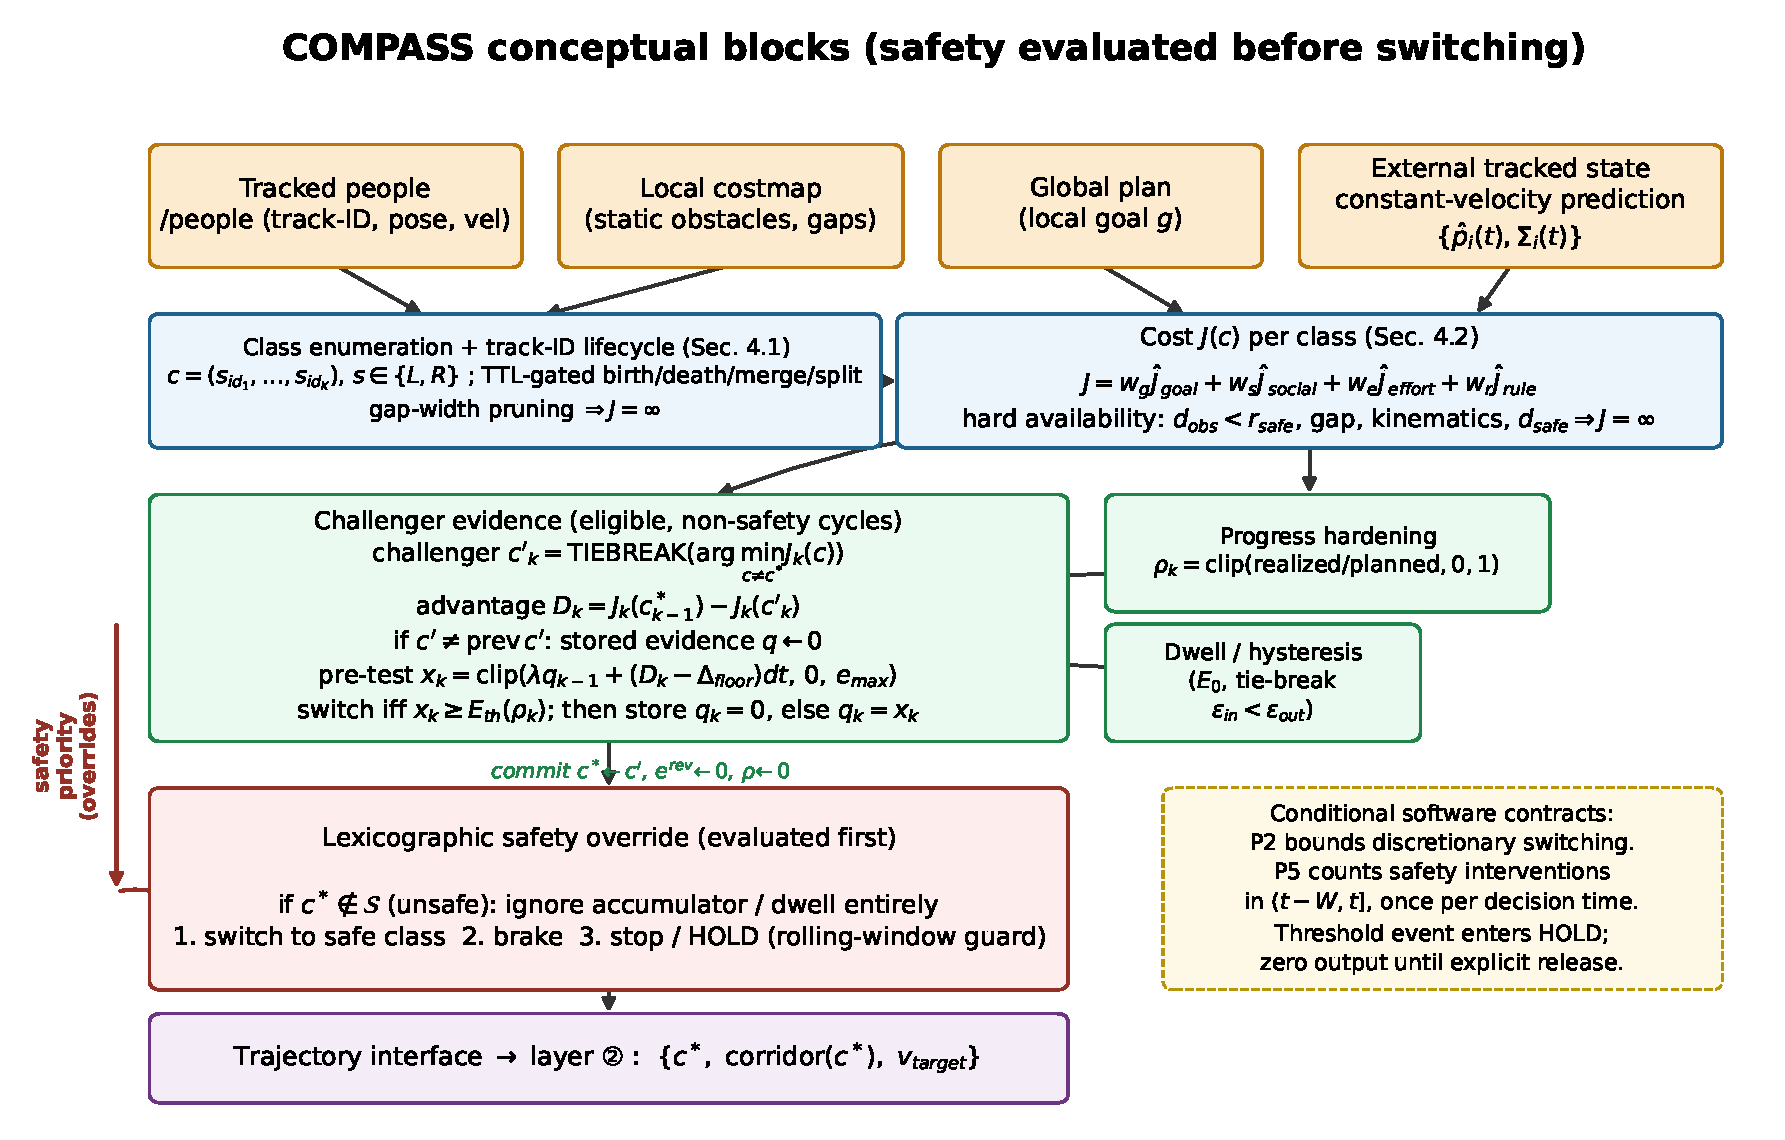
\includegraphics[width=\linewidth]{figures/fig_decision_flow.pdf}
\caption{\textbf{Overview of the \sname\ decision layer.} Conceptual blocks, not a literal execution-order flowchart. Tracked-person, costmap and plan inputs feed class/cost evaluation; safety has priority over discretionary evidence. The diagram distinguishes pre-test evidence $x$ from stored post-reset evidence $q$ and shows P5's conditional rolling-window HOLD contract. The integrated pseudocode (\cref{alg:compass}) specifies the actual control order.}
\label{fig:decisionflow}
\end{figure}


Autonomous serving, delivery, and guide robots are no longer confined to isolated industrial spaces; they now operate in corridors, lobbies, and sidewalks where people move freely. The central difficulty of such shared spaces is not static-obstacle avoidance but \emph{interactive passing decisions} with people who continuously change position and intent. In narrow-corridor head-on encounters, situations where the robot overtakes a person or a person overtakes the robot, and crossing-style traversals, the robot must continually judge ``which side to pass on, whether to proceed or yield, whether to stop.''

Widely used local planners (the \texttt{DWA} family~\citep{fox1997dwa}, \texttt{MPPI}~\citep{williams2017mppi}, \texttt{TEB}~\citep{rosmann2017teb}) re-optimize a cost function at every control cycle. This greedy re-optimization is natural in static environments, but in ambiguous configurations where the costs of the two passing directions are similar, minor sensor noise or a small movement by the person alone can flip the choice from one cycle to the next. As a result, the robot dithers side to side (oscillation) or, unable to commit to either side, comes to a stop --- an outcome reminiscent of the freezing robot problem~\citep{trautman2010}, whose original diagnosis is uncertainty growth rather than commitment failure. Oscillation is not only inefficient --- it also prevents people from reading the robot's intent, undermining both safety and trust. Topology-aware planners recognize the problem but address it through a soft topological-invariance cost~\citep{mavrogiannis2023winding}, an implementation-level selection hysteresis~\citep{rosmann2017teb}, or a consistency parameter formalized at the trajectory-optimization layer~\citep{degroot2024topology}; none of these provides an explicit commitment rule at the discrete decision layer together with a provable bound on how often the passing decision may legitimately flip (\cref{sec:related}).

We study insufficient temporal inertia in the passing decision as one mechanism that can contribute to oscillation; this does not exclude perception, prediction, or interaction uncertainty as other causes. To overcome it, we introduce \emph{\sname}, a decision-layer planner that adds explicit temporal consistency to the passing decision itself (\cref{fig:decisionflow}). The intuition mirrors human walking behavior: once a person decides which way to step aside, they tend to hold that direction, changing it only for a clear reason, and stopping immediately when it becomes dangerous. A related intuition --- that committing to a passing direction aids mutual coordination --- appears in the social-navigation literature as social momentum~\citep{mavrogiannis2022momentum}, and \sname\ embodies the ``hold a once-chosen direction'' behavior as an explicit formal rule at the decision layer. Concretely, \sname\ makes three contributions:
\begin{itemize}
\item \emph{ID-Indexed Topological Classes}: By binding the identity of a passing direction to a person's track ID rather than to a flickering geometric gap, we consistently identify ``the corridor chosen last cycle'' at every cycle. The spawning, removal, merging, and splitting of \Class{es} caused by people entering, leaving, clustering, and separating are specified via explicit lifecycle rules and TTLs, as design contracts that the current implementation only partially realizes (\cref{subsec:enum}).
\item \emph{Unified Commitment Switching with Lexicographic Safety}: The switching margin (hysteresis), dwell (persistence), and progress hardening (point of no return) are folded into a single leaky evidence accumulation equation, with safety placed lexicographically above it. Discretionary changes are deliberately slow (``not rushed''), while the safety override is never delayed by commitment inertia (\cref{subsec:switch,subsec:safety}).
\item \emph{Formal Properties with Offline Validation}: We state anti-oscillation (P1), switching-rate bound (P2), safety dominance (P3), maneuver completion (P4), and conditional finite-window escalation to HOLD (P5) as propositions. The load-bearing anti-oscillation guarantee is P2: a deterministic lower bound of $N_{\min} = \lceil \Eth(\rho)/((D_{\max}-\Dfloor)\,dt)\rceil$ control cycles on the interval between consecutive discretionary switches for fixed $dt$ and zero post-switch evidence, holding on every sample path under the range bound $D_k \le D_{\max}$ that the $[0,1]$ cost normalization of \cref{subsec:cost} supplies by construction, and informative under the declared design condition $E_0 > (D_{\max}-\Dfloor)\,dt$ ($N_{\min} \ge 2$; \cref{rem:p2nonvac}). Because P2 is an upper bound on the switching rate and says nothing about switches occurring, we pair it with a conditional response-time bound (\cref{prop:p2live}): the finite deadline applies only while the same challenger remains selected and eligible, updates proceed without reset or HOLD, its advantage stays above the stated lower bound, and the clip/leak equilibrium has sufficient threshold headroom. P1 refines this, for i.i.d.\ challenger advantages, to an exponentially small per-cycle switching probability and per-unit-time switching rate, proved via Lindley domination and Kingman's bound, with the exponent given by the exact Lundberg root $\theta^*$ of the increment law (the closed form $\theta^* \approx 2\Dfloor/(\sigma_D^2\,dt)$ is retained as tuning guidance only); the exponential form is conditional on that independence hypothesis (\cref{subsec:props}). P4 is proven, on top of the progress $\rho$ dynamics and a lower bound on the lateral progress rate, via a reachable-upper-bound containment condition on the challenger accumulator $\Erev$. Verification is split into two tiers. The decision layer's behavioral consistency, a decision-stream observer statistic, and cyclic latency are \emph{measured} using an offline harness that drives the actual decision core (\cref{sec:exp}); performance metrics requiring physical simulation or a real robot, along with external baselines and user studies, are left as planned evaluations (\cref{app:planned}) specified via a pre-registered protocol.
\end{itemize}

We evaluate \sname\ in an offline harness that drives the actual decision core over 5 reproducible encounter scenarios $\times$ 50 seeds against internal comparators and knob ablations. In the ambiguous-tie scenario, the immediate-argmin comparator changes its decision 98.16 times per 10~s encounter on average, whereas \sname\ keeps its commitment with zero changes; across all 250 trials \sname\ averages 0.40 decision changes per encounter against 29.74 for argmin, and no trial exceeds one change (\cref{tab:main,tab:scenario}). The ablations also correct a prior hypothesis: removing the hysteresis margin or progress hardening alone produces no observed regression in this regime, so the leaky accumulator itself is the primary oscillation-suppression mechanism. A historical decision-core-only timing run gives p99 $58.6\,\mu$s and max $651.3\,\mu$s at $K=3$ (8 classes), about $1.30\%$ of a 20~Hz period. These results establish the conditional decision rule and its offline behavioral consistency; they do not measure physical safety, human-perceived legibility, or comparison against external planners, which remain the pre-registered next step.

\section{Related Work}\label{sec:related}

\noindent\textbf{Local Planners and Topological Consistency.} \texttt{DWA}~\citep{fox1997dwa} selects a velocity command from a dynamic window at every cycle; each cycle's selection is made anew, with no memory of previous decisions, so nothing in the scheme itself discourages the chosen side from flipping between cycles (a structural observation of ours, not a claim made by \citet{fox1997dwa}). \texttt{TEB}~\citep{rosmann2017teb} maintains and optimizes several topological alternatives in parallel; its ROS implementation adds a selection-cost hysteresis that discourages switching between alternatives, but this is an implementation-level heuristic --- the formulation itself does not define commitment across cycles. \texttt{MPPI}~\citep{williams2017mppi} is a sampling-based MPC formulation; it does not treat the discrete structure of social passing decisions as first class. H-signature-based enumeration of homotopy classes~\citep{bhattacharya2012topological} rigorously represents the topological identity of a path but focuses mainly on static-obstacle topology; the branch that extends this topological view to moving-pedestrian environments is most relevant to this paper. Topological braids model the joint avoidance strategy of several agents, and a planner can then comply with the avoidance intentions inferred from their past behavior~\citep{mavrogiannis2019braids}. Dynamic Channel~\citep{cao2019dynamicchannel} is a real-time crowd-navigation framework that searches a triangulated spatial graph, combining pedestrian dynamics with topological-corridor selection; it picks one topology per planning cycle but does not formalize the temporal consistency of that choice via an explicit commitment rule or switching-rate guarantee. Winding Through~\citep{mavrogiannis2023winding} tracks the homotopy class the robot's path holds relative to each pedestrian and penalizes changes to that class over time as a cost --- being motivated by suppressing passing-side switches, it is among the closest prior work, but it operates as a soft topological-invariance cost internal to the planner and does not define a track-ID-indexed \Class\ lifecycle or a provable switching-rate bound. Topology-driven parallel trajectory optimization~\citep{degroot2024topology} runs local MPC optimizers seeded in different homotopy classes in parallel for dynamic obstacles and commits to the best resulting trajectory each cycle, maintaining consistency of the chosen class --- this treats homotopy consistency via parallel search at the trajectory-optimization layer, and does not provide an explicit accumulator-based commitment rule at the discrete decision layer nor a formal switching-rate guarantee for it. SHINE~\citep{martinezbaselga2026shine} selects among topologically distinct guidance trajectories with a network trained on human motion data and reduces the selection cost of the homology class followed in the previous control period by a consistency weight, stating explicitly that fast switching between topology classes can lead to indecisive and ultimately non-social navigation. SHINE therefore treats decision oscillation in social navigation as a design problem; its remedy is a one-step, previous-class cost bias, and it does not state a bound on switching frequency. \citet{zhou2023minimally} keep the previously selected trajectory as a candidate with a time-decaying weight, motivated by the observation that a high decision frequency, together with perception noise, can keep pedestrians from discerning a stable intention and cause oscillation. In multi-agent navigation, a learned planner can choose target winding numbers that a model-predictive controller then realizes~\citep{nakao2025wnummpc}, a decision--control split aimed at breaking symmetry deadlocks rather than at bounding switching. \sname\ differs from these mainly in making the cross-cycle commitment rule itself, rather than a per-cycle cost bias, the object of analysis, and in specifying \Class\ correspondence over time (lifecycle) against track identity.

\noindent\textbf{Explicit Passing-Side Decisions and Opinion Dynamics.} Opinion-dynamics navigation makes the passing side an explicit decision state. \citet{cathcart2023opinion} drive human--robot corridor passing with nonlinear opinion dynamics in which the robot forms an opinion about which side to pass an approaching person; they show analytically that deadlock in the decision is broken when the robot's attention exceeds a critical value, even when the robot has no bias or evidence for either side, and that opinions form rapidly; they validate these predictions in human--robot experiments. Opinion dynamics has also been combined with vortex fields so that robot and humans reach a consensus on the direction of motion~\citep{daddato2024oval}, and with dynamical-system modulation so that the robot chooses a passing side from onboard sensing, with simulation and human-participant experiments~\citep{chen2025socialdsm}. These methods are the closest prior work on a stateful, analyzed decision layer for the passing side. The formal target of \citet{cathcart2023opinion} is the formation of a decision (deadlock breaking); that of \sname\ is a bound on how often a formed decision is revised, over multi-person track-indexed labels. \sname\ has no comparable human or closed-loop evidence. Concurrently with this work, BIG-CBF~\citep{li2026bigcbf} separates maneuver selection from safety enforcement: it selects among six closed-loop behaviors, including passing left and right, with a switching cost relative to the retained mode, a minimum dwell time and a relative switching-improvement threshold, gives a hard control-barrier-function filter final safety authority, and reports closed-loop simulation and physical-robot experiments. BIG-CBF thus covers mode retention, dwell and improvement gating, and safety priority, with much broader empirical evidence than this paper; it does not use an evidence accumulator, a progress-dependent threshold or track-indexed topological classes, and we did not find a stated switching-frequency bound in it.

\noindent\textbf{Change Detection, Switching Logic, and Arbitration.} The mathematics used in this paper is standard. Page's cumulative-sum (CUSUM) inspection scheme~\citep{page1954cusum} accumulates the deviations of observations from a reference value and signals when the cumulative sum rises by a decision interval above its running minimum; in recursive form this is a sum reflected at zero. With the leak removed and a constant threshold, the accumulator of \cref{subsec:switch} is this statistic, written as Lindley's queueing recursion~\citep{lindley1952queue}, and the exponential bound of P1 is the classical tail bound for that recursion~\citep{kingman1970queues}. Leaky accumulation of evidence toward a threshold is a standard model of perceptual choice~\citep{usher2001lca}. In supervisory control, hysteresis switching logic changes the active candidate only when its monitoring signal reaches $(1+h)$ times the smallest one, for a hysteresis constant $h>0$, and yields a bound on the number of switches on an arbitrary time interval~\citep{hespanha2003hysteresis}; dwell-time switching separates consecutive switches by at least a prescribed interval, and an average dwell-time bounds the number of switches on any interval by a chatter bound plus a term linear in the interval length~\citep{hespanha1999dwell}. P2 is a dwell-time guarantee of this kind for the discretionary branch, obtained by an elementary bounded-increment argument. Finally, placing a safety behavior strictly above nominal behaviors is standard priority-based behavior arbitration~\citep{orzechowski2020arbitration}, which has been extended with verification and fallback layers~\citep{spieker2024arbitration}. We use these results as tools and claim neither the accumulator nor its bounds as new mathematics.

\noindent\textbf{Human Models, Prediction, and Learned Social Costs.} The Social Force Model~\citep{helbing1995social} describes pedestrian motion as interaction forces, and \texttt{ORCA}/\texttt{RVO}~\citep{vandenberg2011rvo} formalizes reciprocal multi-agent collision avoidance; social-navigation work that addresses freezing models such human reactivity and cooperation explicitly~\citep{trautman2010,trautman2015dense}. Proxemics~\citep{hall1966hidden} contributes qualitative, culture-dependent interpersonal distance zones, which robotics work has operationalized as cost fields --- notably the asymmetric-Gaussian formulation of \citet{kirby2010thesis}. Learning-based probabilistic predictors --- Social-LSTM~\citep{alahi2016sociallstm}, Social-GAN~\citep{gupta2018socialgan}, Trajectron++~\citep{salzmann2020trajectron} --- predict a person's future trajectory as a distribution, and the line of work that learns socially compliant costs and prediction models from pedestrian trajectory features via maximum-entropy inverse reinforcement learning~\citep{kuderer2012feature,kretzschmar2016irl} models human cooperative avoidance behavior as a trajectory distribution (including a mixture distribution over joint path choices), generating robot trajectories that conform to observed walking conventions. While these provide rich human models and learned cost/prediction models for trajectory generation, the works cited in this paragraph do not treat the oscillation of the robot's decision itself as a measurement target or design goal, nor state switching-rate bounds for a discrete passing decision. Learned topology selection differs in this respect: SHINE~\citep{martinezbaselga2026shine} explicitly treats fast class switching as a design problem (first paragraph of this section). \sname\ adopts such cost fields as input and uses a Kalman constant-velocity prediction over a short horizon (\cref{subsec:formulation,sec:disc}); the learned predictors can be incorporated as a replaceable input module, since this contribution is orthogonal to the choice of predictor --- only the mean-trajectory and covariance input need be replaced.

\noindent\textbf{Social Momentum, Legibility, and Group Awareness.} Cooperation-aware navigation that jointly models robot and human trajectories in planning~\citep{trautman2015dense} addresses cooperative navigation amid dense crowds. In particular, social momentum~\citep{mavrogiannis2022momentum} scores candidate actions by the angular momentum of the joint robot--human configuration to reconcile human--robot passing-side intentions and reinforce implicit coordination; it is a per-cycle objective rather than a persistent accumulator, but it articulates the intuition --- committing to a passing side aids coordination --- that \sname\ formalizes as an explicit scalar evidence accumulator. Legible/predictable motion~\citep{dragan2013legibility} presents the view that robot motion should reveal intent to an observer; the commitment mechanism of \sname\ suppresses oscillation of the discrete decision label, which we hypothesize can support legible motion; this paper does not show it, because the offline observer scores decision-label streams only (\cref{subsec:setup}) and motion legibility is not measured. The methodology for human validation of legibility is elaborated via the observer model of \cref{subsec:observer} together with the user-study protocol of \cref{app:planned}. Metrics for human comfort and social appropriateness are undergoing standardization in social-navigation surveys~\citep{mavrogiannis2023survey,gao2022evaluation,francis2023principles}, and \sname\ takes the axes of decision oscillation and legibility as its quantitative target among these. The spatial arrangement people form during conversation/interaction (F-formation) was formalized by \citet{kendon1990conducting} via the concepts of o-space and p-space; treating such formations as ``groups that must not be split'' is a norm adopted in robot navigation, not part of Kendon's own definition, and detecting and respecting F-formations has been treated as a core element of group-aware navigation~\citep{riosmartinez2015survey}. Automatic F-formation detection itself is outside the scope of this paper and is assumed to be provided by an external perception module; \sname\ extends the merge rule of \cref{subsec:enum} to interaction-based groups so as to avoid splitting F-formations (\cref{subsec:groups}).

\noindent\textbf{Positioning.} The problem of temporal consistency on the passing side has been recognized in prior work, with mechanisms of varying explicitness --- a soft topological-invariance penalty~\citep{mavrogiannis2023winding}, the selection-cost hysteresis in the ROS implementation of \texttt{TEB}~\citep{rosmann2017teb}, per-cycle topological-corridor selection~\citep{cao2019dynamicchannel} (one corridor is chosen each cycle, but no cross-cycle commitment is defined), the social-momentum objective~\citep{mavrogiannis2022momentum}, and previous-trajectory retention~\citep{zhou2023minimally}. \citet{degroot2024topology} \emph{do} formalize inter-cycle topological consistency: a consistency parameter trades off following the previously selected homotopy class against switching to a better one, and at one extreme enforces the previous class as long as it remains valid; SHINE applies a previous-class consistency weight in social navigation for the stated purpose of avoiding indecisive navigation~\citep{martinezbaselga2026shine}. Opinion-dynamics methods make the passing side an explicit, stateful decision with analytical deadlock-breaking guarantees~\citep{cathcart2023opinion}, and concurrent work combines passing-mode retention, dwell and relative-improvement gating, and a hard safety filter in closed loop~\citep{li2026bigcbf}. The mechanisms and mathematics we use are also standard (see Change Detection, Switching Logic, and Arbitration above). The delta of this paper is therefore narrow, and we state it precisely: (i) a leaky, CUSUM-type evidence accumulator with a progress-dependent threshold, used as the commitment rule for a social passing decision; (ii) an explicit switching-frequency contract for that decision --- the deterministic, pathwise inter-switch bound P2, its conditional exponential refinement P1, and the conditional response-time bound --- stated together with the assumptions each needs; (iii) a track-ID-indexed \Class\ representation with lifecycle rules (spawn, removal, merge, split, TTL), which defines consistency against person identity rather than against a geometric homotopy class recomputed from the current scene, specified as a design contract that the current implementation only partly realizes; and (iv) an open ROS~2 Nav2 controller plugin with an offline harness whose ablations indicate that, in the tested regime, the accumulator rather than the margin or progress hardening carries the oscillation suppression. To the author's knowledge, no prior social-navigation work states a switching-frequency bound for the discrete passing decision. We claim neither the individual mechanisms nor the mathematics as new, and we have not compared against consistency-weight, opinion-dynamics or dwell-plus-hysteresis baselines (\cref{sec:disc}).

\section{\sname: Commitment-Based Passing Decisions at the Decision Layer}\label{sec:method}

\sname\ is a decision-layer planner: at every control cycle it chooses which topological passing \Class\ to commit to, and whether to proceed, decelerate, stop, or hold, before a trajectory layer instantiates that choice. We first formulate the decision problem and its assumptions (\cref{subsec:formulation}). \sname\ then enumerates track-ID-indexed topological classes and keeps them in correspondence across cycles (\cref{subsec:enum}), scores each class with a normalized, asymmetric social cost (\cref{subsec:cost}), accumulates the challenger's advantage in a single leaky evidence variable that governs discretionary switching (\cref{subsec:switch}), and overrides that rule lexicographically whenever the committed class becomes unsafe (\cref{subsec:safety}). \Cref{subsec:algo} integrates these stages into one control cycle (\cref{alg:compass}) and states the implemented interface. \Cref{subsec:props} states and proves the five properties P1--P5; \cref{subsec:observer,subsec:groups,subsec:leak} define the legibility observer, the group and vulnerable-pedestrian extensions, and the analysis of the leak against a simple dwell timer.

\subsection{Formulating the Decision Layer: Layers, Assumptions, and Objective}\label{subsec:formulation}

\noindent\textbf{Layer separation.} We separate social navigation into three layers. (i) The \emph{decision layer} --- the layer that determines discrete intents such as which side to pass on, and whether to yield, proceed, overtake, or stop. (ii) The \emph{trajectory layer} --- the layer that instantiates a given decision as a curvature-continuous ($G^2$) trajectory. (iii) The \emph{presentation layer} --- the layer that visually reveals the planned trajectory to people (e.g., an AR overlay). The contribution of this paper lies entirely in the decision layer; the ideal trajectory interface is a design assumption, not an end-to-end validation claim for the current adapter (implementation scope in \cref{subsec:algo}).

\noindent\textbf{Notation.} Let $k$ denote the control cycle and $dt$ the cycle interval. Let $\mathcal{C}_k$ denote the set of candidate topological \Class{es} at cycle $k$, and let $J_k(c) \in \mathbb{R}^+ \cup \{\infty\}$ denote the representative trajectory cost of class $c$ ($\infty$ when unavailable). Let $c^*_{k-1}$ denote the previously committed \Class, and let $\mathcal{S}_k = \{c \in \mathcal{C}_k : \mathrm{Safe}_k(c)\}$ denote the safe/available set. Prediction of person $i$ is provided by a Kalman constant-velocity estimator, giving a mean trajectory $\hat p_i(t)$ and covariance $\Sigma_i(t)$, where $\Sigma_i(t)$ grows with the prediction horizon. A notation table is given in \cref{app:notation}.

\begin{assumption}[Assumptions and scope]\label{asm:scope}
(a) Planar (2D) navigation. (b) A short prediction horizon $[0,T]$ (typically 2--4 seconds). (c) Person tracking and data association are provided by an external module. (d) The trajectory generator, given a \Class, corridor, and target speed, is assumed capable of generating a trackable trajectory and of realizing a commanded \emph{cross-track progress rate} of at least $v_{\text{lat,min}} > 0$ (used in P4). Here $v_{\text{lat,min}}$ is not the vehicle body's lateral (swerve) velocity but the per-unit-time progress rate of the cross-track coordinate toward the planned lateral offset; for non-holonomic drives (differential, Ackermann) it is realized as the product of forward speed and steering (curvature), while for holonomic drives it is realized as a direct lateral-velocity component. Hence $v_{\text{lat,min}} > 0$ presupposes forward clearance and a positive forward speed. (e) Pedestrian passing conventions (e.g., right-side passing) are a locale setting and are not assumed to be a universal constant (\cref{subsec:cost}, \cref{app:sensitivity}).
\end{assumption}

\noindent\textbf{Objective.} A decision policy maps, at each cycle, the retained decision state and the current $(\mathcal{C}_k, J_k, \mathcal{S}_k)$ to a committed class $c^*_k$, a target speed, and a mode. For cycles $s<t$, write
\begin{equation}
N^{\mathrm{disc}}_{(s,t]} \;=\; \sum_{k=s+1}^{t} \mathbb{1}\!\left[\,c^*_k \neq c^*_{k-1}\ \text{and the change is made by the discretionary branch}\,\right]
\label{eq:objective}
\end{equation}
for the number of discretionary decision changes in $(s,t]$; changes made by the safety branch are not counted. We design a decision policy that prioritizes the supplied safety/availability predicates at every active decision cycle and bounds the discretionary decision changes counted by \eqref{eq:objective}. Physical safety, motion legibility, goal progress, and social comfort require independent validation and are not guaranteed by branch priority.

\subsection{Enumerating Topological Classes: Cross-Cycle Correspondence by Track ID}\label{subsec:enum}

\textbf{Enumeration.} We index the $K$ relevant agents (typically 1--3) within the radius of influence and prediction horizon by track ID. The \Class\ label is defined as a vector of left/right passing signs over each relevant agent. The lifecycle and winding-sign procedures below are intended design contracts; the current input-order top-K implementation is distinguished explicitly at the end of this subsection and in \cref{subsec:latency}.
\begin{equation}\label{eq:classlabel}
c = (s_{\mathrm{id}_1}, \ldots, s_{\mathrm{id}_K}), \qquad s \in \{L, R\}
\end{equation}
Among the up to $2^K$ combinations, any combination whose corresponding corridor width is narrower than the sum of the robot's width and the safety margin is immediately pruned with $J = \infty$. This corridor-width comparison presupposes a \textbf{circular-footprint approximation} (treating the robot's width as an orientation-independent constant); for elongated rectangular footprints, the occupied area varies with orientation during rotation, making pruning and availability decisions conservative, which we discuss separately in \cref{sec:disc} (rectangular-footprint conservatism). The left/right sign of each \Class\ is computed from the winding sign (cross-product integral or H-signature integral) by which the representative path winds around the predicted human positions. Front/rear (temporal-axis) passing is not treated as a separate \Class\ but handled through the asymmetric social cost of \cref{subsec:cost}. A more rigorous spatiotemporal homotopy extension is discussed as future work in \cref{sec:disc}. The combinatorial explosion of enumeration and the analytical bound on the number of effective \Class{es} after pruning are analyzed in \cref{subsec:latency}.

\textbf{Cross-cycle correspondence (key).} For ``retain the previous $c^*$'' to be meaningful, $c^*$ must be re-identified every cycle. Because \Class\ identity is bound to track IDs rather than geometry, correspondence reduces to label matching such as ``right of agent \#7, left of agent \#12,'' which rides for free on IDs already provided by the tracking module. The design specifies the following lifecycle rules (\cref{fig:lifecycle}).

\begin{itemize}
\item \textbf{Creation} (a relevant agent enters, or a new corridor appears): a new \Class\ appears as a challenger but starts from evidence $e=0$, so there is no immediate jump.
\item \textbf{Extinction} (a relevant agent leaves): the corresponding dimension is removed from all labels. If $c^*$ was distinguished solely by that person, it is absorbed into a coarser \Class; progress $\rho$ is retained if the actual path is unchanged, and reset if it changes.
\item \textbf{Temporary unavailability} (corridor closes, $J=\infty$): identity is retained but passage is momentarily blocked. If $c^*$ is affected, the safety override takes over, and the identity is remembered for a short TTL so that a momentary flicker does not break the commitment.
\item \textbf{Merge} (two people form one cluster): the two dimensions collapse into one, leaving only the sign shared by both sides, with ``between'' becoming $\infty$. The old $c^*$ is mapped to the surviving coarser \Class. Merge decisions use not only spatial proximity but also interaction cues (mutual stillness, mutual orientation, sustained proximity); details are given in \cref{subsec:groups}.
\item \textbf{Split} (a cluster separates): the reverse process --- the old $c^*$ is mapped to the child that is consistent with the robot's current lateral offset and heading.
\end{itemize}

\begin{figure}[t]
\centering
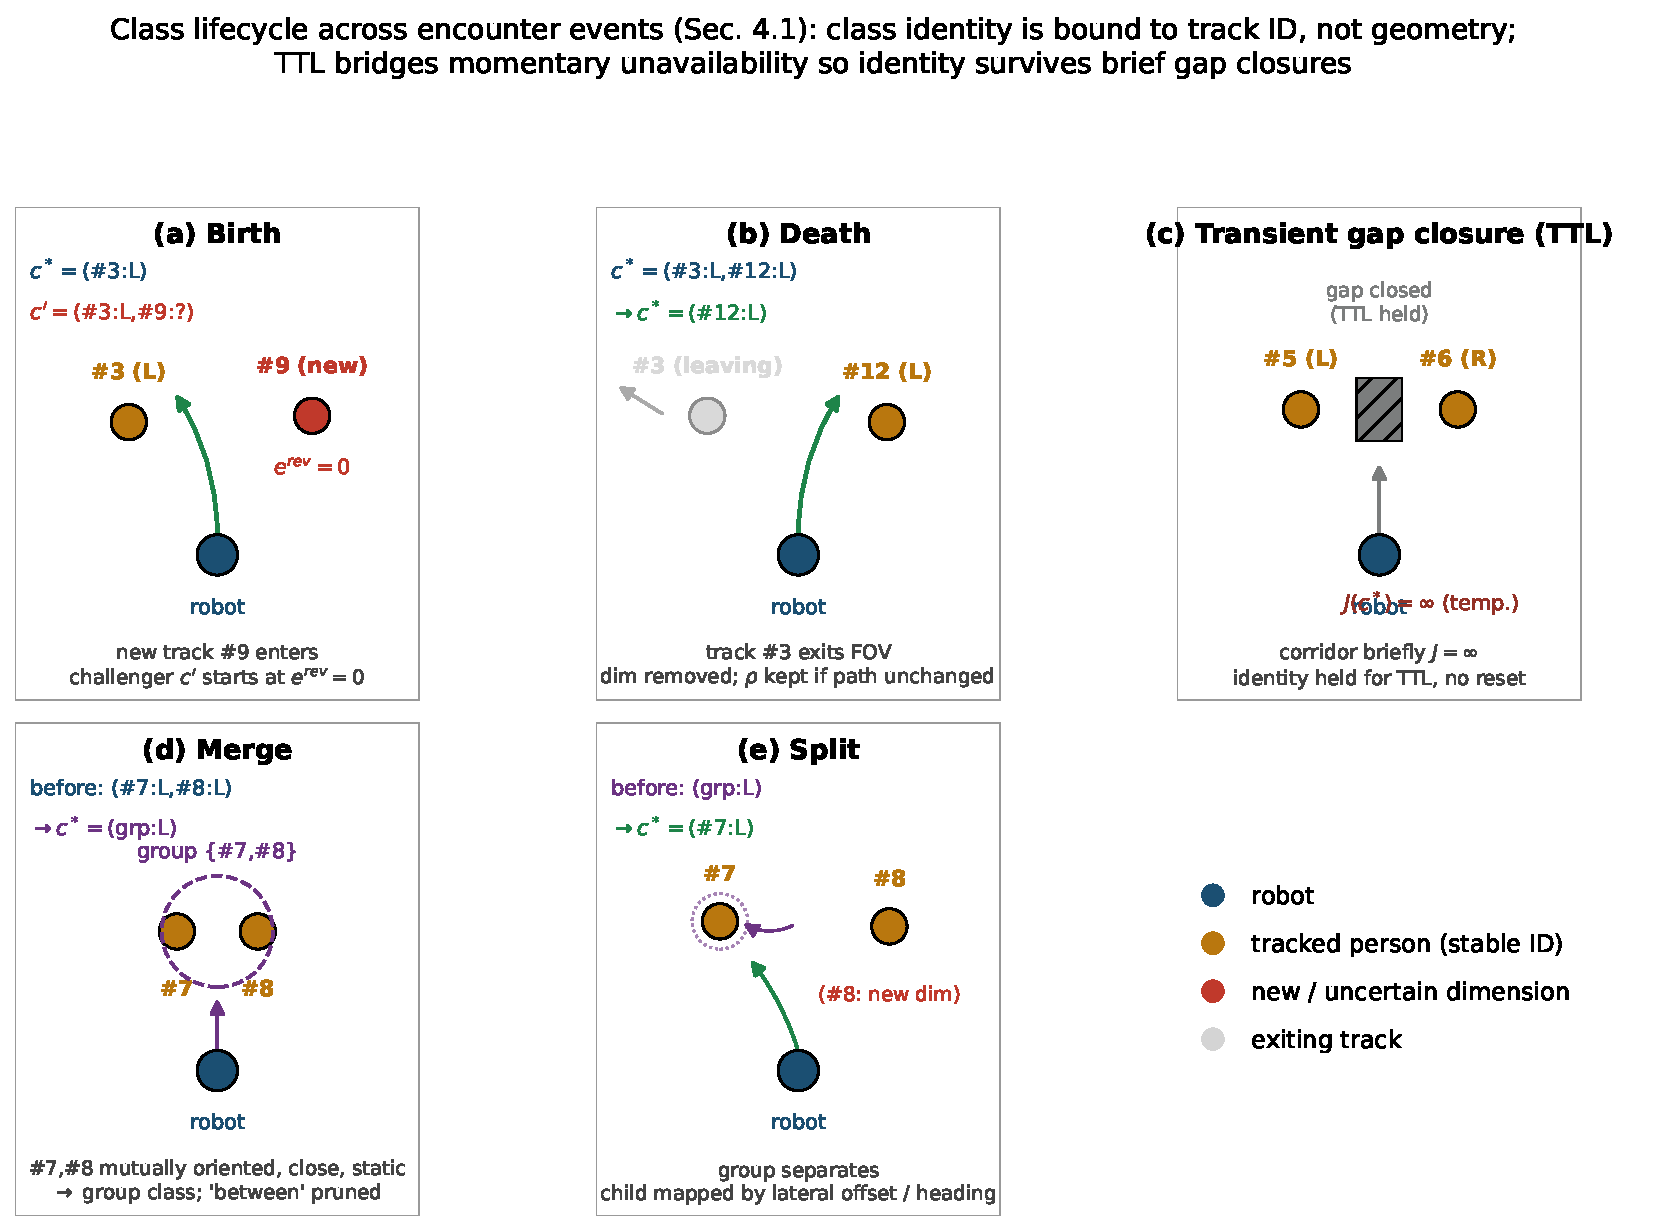
\includegraphics[width=\linewidth]{figures/fig_class_lifecycle.pdf}
\caption{\textbf{Lifecycle events of a topological class} (schematic). (a) Creation --- a new track appears as a challenger, starting from $\Erev=0$; (b) Extinction --- when a track leaves, the corresponding dimension is removed ($\rho$ is retained if the path is unchanged); (c) Temporary unavailability --- even when a corridor momentarily becomes $J=\infty$, identity is retained for a TTL to prevent a reset; (d) Merge --- two people judged by interaction cues (mutual orientation, proximity, low speed) merge into a single group class; (e) Split --- a group separates, mapped to the child class consistent with the robot's lateral offset and heading. Class identity is bound to human track IDs rather than geometry.}
\label{fig:lifecycle}
\end{figure}


These lifecycle rules specify the intended correspondence layer. The current decision-core enumeration constructs labels for the first $K_{\rm cap}$ input tracks; the presence of label operations does not establish an integrated TTL, merge/split, winding-sign, or group-lifecycle manager. The offline two-label harness holds track identity fixed, so it validates neither those lifecycle rules nor their effect in a tracker. The accumulator is the implemented and measured temporal decision mechanism.


\subsection{Scoring Classes: A Normalized Asymmetric Social Cost}\label{subsec:cost}

\begin{figure}[t]
\centering
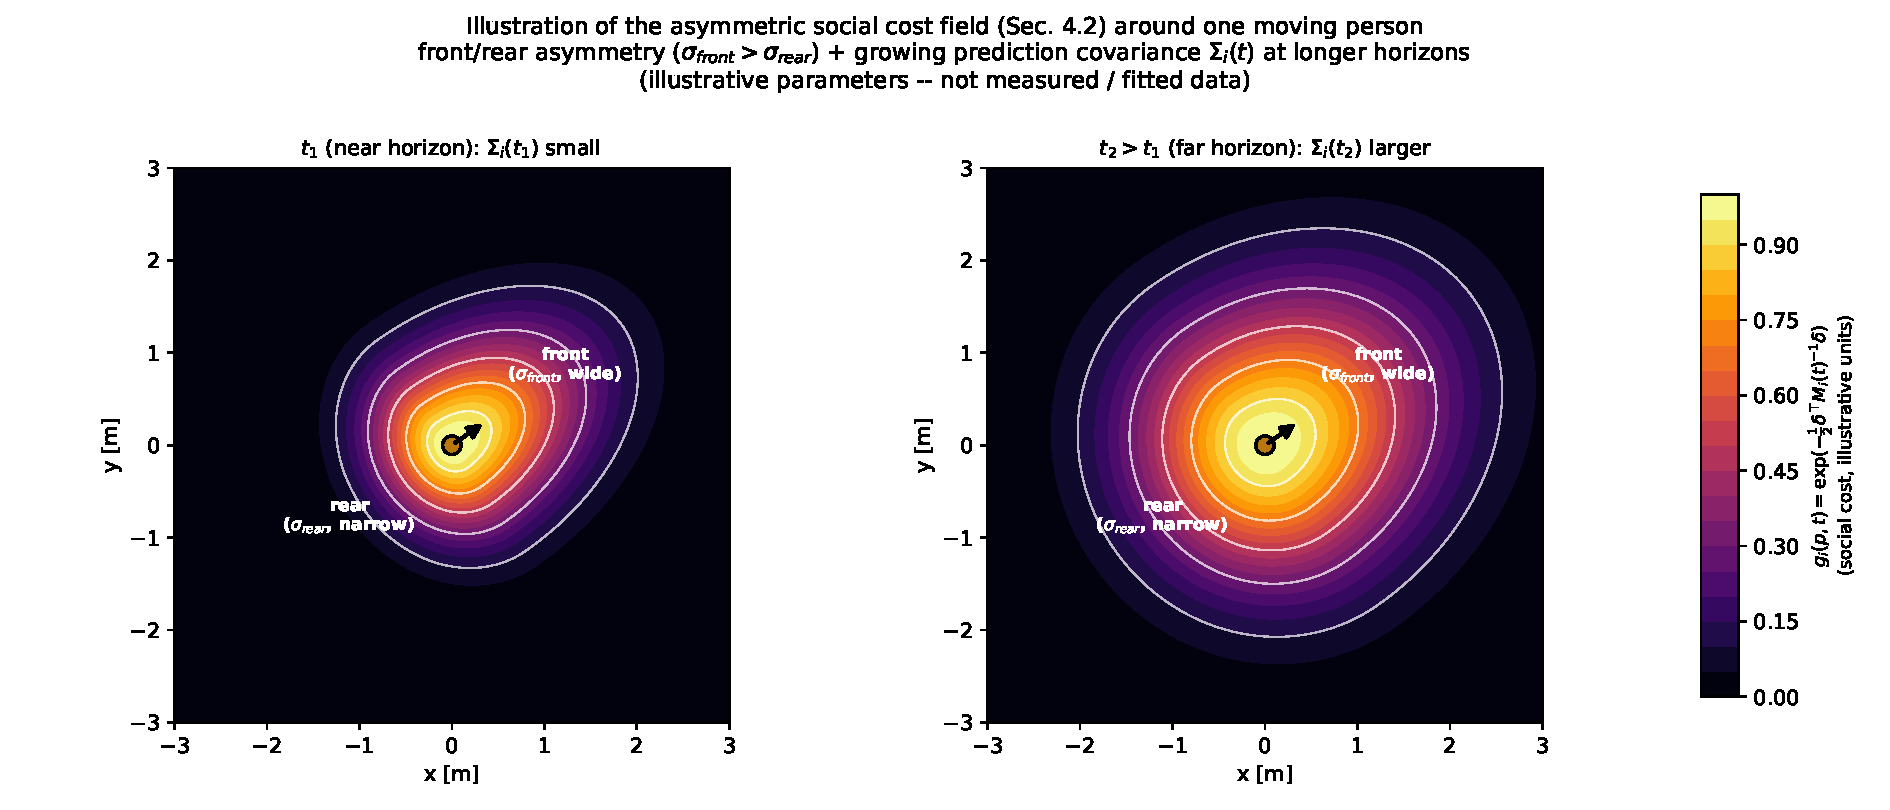
\includegraphics[width=0.85\linewidth]{figures/fig_social_cost_field.pdf}
\caption{\textbf{Asymmetric social cost field} of \cref{subsec:cost}, $g_i(p,t) = \exp(-\tfrac12 \delta^\top M_i(t)^{-1}\delta)$ (a schematic based on the formula, not measured data). Left: near horizon $t_1$ (small predictive covariance $\Sigma_i(t_1)$); right: far horizon $t_2 > t_1$ ($\Sigma_i(t_2)$ grows, expanding the personal-space ellipse). Both panels show the front/rear asymmetry $\sigma_{\text{front}} > \sigma_{\text{rear}}$ (front personal space wider than rear), with half-plane assignment determined by projecting $\delta$ into local coordinates referenced to the person's heading.}
\label{fig:socialcost}
\end{figure}


The cost of each \Class\ is defined as a weighted sum integrated over the horizon $[0,T]$ along the representative trajectory $\tau_c$.
\begin{equation}\label{eq:cost}
J(c) = w_g J_{\text{goal}} + w_s J_{\text{social}} + w_e J_{\text{effort}} + w_r J_{\text{rule}}, \qquad J(c) = \infty \text{ if unavailable}
\end{equation}

\begin{itemize}
\item \textbf{Progress $J_{\text{goal}}$.} Distance from the local goal $g$ at the end of the horizon: $J_{\text{goal}} = \lVert p_r(T) - g \rVert$. This penalizes detour/stopping \Class{es}.
\item \textbf{Asymmetric social cost $J_{\text{social}}$.} A proxemics cost field is laid over each person and integrated for intrusion (\cref{fig:socialcost}).
\begin{align}
J_{\text{social}} &= \sum_i \int_0^T g_i(p_r(t), t)\, dt \\
g_i(p,t) &= \exp\!\left(-\tfrac{1}{2}\, \delta^\top M_i(t)^{-1} \delta\right), \qquad \delta = p - \hat p_i(t) \\
M_i(t) &= R_i(t)\, \mathrm{diag}(\sigma_h^2, \sigma_s^2)\, R_i(t)^\top + \Sigma_i(t)
\end{align}

Here the heading component $\sigma_h$ is set to be front/rear asymmetric ($\sigma_{\text{front}}$ for the front half-plane, $\sigma_{\text{rear}}$ for the rear). This makes the cost of cutting in front of a person differ from that of passing behind them, so that the choice of passing side aligns with social norms. \textbf{$\sigma_{\text{rear}}$ appears in two distinct mechanisms in this paper and must be distinguished. (i) As the base shape of the cost-field asymmetry, $\sigma_{\text{front}} > \sigma_{\text{rear}}$ (the static shape in which the front personal-space region is wider than the rear), and (ii) as a contextual upward adjustment in the overtaking regime (a dynamic adjustment that deliberately raises the rear cost to suppress the surprise of a blind-spot approach) --- these are distinct operating principles: the former induces yielding to the rear in head-on encounters, and the latter suppresses rear approach during overtaking/close passing.} In addition, the predictive covariance $\Sigma_i(t)$ is added to the cost field, so that the personal-space ellipse widens further into the future and the robot gives wider berth accordingly. $\sigma_s$ determines the lateral width. Which of $\sigma_{\text{front}}$ or $\sigma_{\text{rear}}$ applies to a given person is computed from that person's heading and the robot--person relative motion. That is, $\sigma_{\text{front}}$ is applied in the head-on-encounter regime where the robot crosses the person's front half-plane, and $\sigma_{\text{rear}}$ is applied in the overtaking regime where the robot enters the person's rear half-plane; half-plane assignment is determined by projecting $\delta$ into local coordinates referenced to the person's heading. \textbf{Here, the $\sigma_{\text{rear}}$ regime switch (head-on encounter $\leftrightarrow$ overtaking) is not driven by a separate variable but by the same variable as the rear half-plane projection judgment above (the sign of $\delta$'s local projection onto the person's heading) --- that is, the selection of the cost-field asymmetry and the assignment to the overtaking regime are consistently derived from a single judgment.}

\textbf{Parameter grounding and locale configurability.} $\sigma_{\text{front}}$, $\sigma_{\text{rear}}$, $\sigma_s$, and the passing-side preference are not treated as universal constants but as \textbf{locale/culture configuration values}. The basic form of the asymmetric Gaussian proxemics is grounded in Kirby \citep{kirby2010thesis}, and the forward-extended shape draws on Hall's personal-space zones \citep{hall1966hidden} and the social navigation survey \citep{riosmartinez2015survey}. However, we do not adopt the unconditional assumption that ``passing behind is always preferable.'' Since approach from a person's blind spot (rear) can plausibly induce surprise or discomfort --- a design consideration this paper adopts, rather than a finding reported in the surveys cited above --- this cost exposes $\sigma_{\text{rear}}$ as a \textbf{context-dependent knob}, so that (i) rear yielding is preferred in head-on encounters, while (ii) the rear cost is raised during overtaking/close passing to suppress blind-spot entry. The passing-side preference is locale-dependent and configurable (e.g., some pedestrian environments are reported to favor the right, others the left, or a mix). For an experimental study of a single population (Bordeaux, France) showing that avoidance-side conventions in pedestrian crowds can emerge through self-organization, see \citep{moussaid2009experimental}; however, since that study is not a cross-cultural comparison, we do not extrapolate it as direct evidence that ``the passing side varies by culture''; this paper takes the conservative choice of not fixing the passing side as a universal constant but separating it out as a \code{locale.keep\_side} $\in \{\text{right}, \text{left}, \text{none}\}$ setting. The design of the sensitivity analysis for these parameters is described in \cref{app:sensitivity}, and their measurement is left to the planned evaluation (\cref{app:planned}).


\item \textbf{Effort/smoothness $J_{\text{effort}}$.} $J_{\text{effort}} = \int_0^T (\alpha \kappa^2 + \beta a^2 + \gamma \dot\kappa^2)\, dt$. The $\dot\kappa$ (curvature rate) term induces $G^2$ continuity, which directly benefits smooth tracking and the curvature display of the presentation layer.
\item \textbf{Rule $J_{\text{rule}}$.} A soft penalty for pedestrian traffic conventions (preference per \code{locale.keep\_side}) and lane keeping. The design of the sensitivity curve for the weight $w_r$ is given in \cref{app:sensitivity}.
\end{itemize}

\textbf{Hard availability.} $J = \infty$ if any of the following holds: static collision ($d_{\text{obs}} < r_{\text{safe}}$), insufficient corridor width, violation of kinematic limits, or violation of the hard safety distance $d_{\text{safe}}$ from a predicted person. This is a dual structure in which soft discomfort is handled by $J_{\text{social}}$ while physical/safety constraints are handled by hard availability.

\textbf{Normalization, range, and units.} For each term $X$, choose finite calibration bounds with $J_X^{\max}>J_X^{\min}$ and use $\hat J_X=\mathrm{clip}((J_X-J_X^{\min})/(J_X^{\max}-J_X^{\min}),0,1)$. With nonnegative finite weights, available finite costs satisfy $0\le J=\sum_Xw_X\hat J_X\le\sum_Xw_X$, so $|D_k|\le\sum_Xw_X$. Unavailable classes are excluded from discretionary comparison; their infinite cost is not an admissible accumulator input. This bound is a property of the normalized cost path, not of arbitrary externally supplied \code{step\_evals} inputs.

Fixed pre-calibrated constants preserve the meaning of normalized advantage across cycles. If cost units are rescaled, the calibration constants must co-transform to preserve affine invariance; that can be done for fixed constants as well as per-cycle statistics. Per-cycle min--max statistics instead change the raw-cost margin with the candidate range: a narrower range requires a \emph{smaller}, not larger, raw-cost difference to exceed the same normalized $\Dfloor$. That changes its semantic interpretation, but P2 still holds whenever its stated normalized advantage bound holds. P1 separately requires its explicit distributional hypotheses.

$J$, $D_k$ and $\Dfloor$ are dimensionless under normalized weights. Because updates multiply by $dt$ measured in seconds, evidence $e$, $E_0$ and $e_{\max}$ have normalized-cost--second units; $\lambda$, $k_\rho$, $\rho$ and $p$ are dimensionless, and $\theta^*$ has reciprocal-evidence units. Hence $\theta^*E_0$ is dimensionless. The value $\Dfloor=0.05$ is five percent of one unit-weight normalized term, not five percent of the full weighted range when $\sum_Xw_X=2.8$. The numerical knob values and reported experiments are unchanged by making these units explicit.


\subsection{Accumulating Evidence: A Commitment Switching Rule}\label{subsec:switch}

Let the challenger be $c'_k = \operatorname*{argmin}_{c \in \mathcal{S}_k,\, c \ne c^*} J_k(c)$, and the challenger advantage $D_k = J_k(c^*_{k-1}) - J_k(c'_k)$. We fold the margin, dwell, and progress hardening into a single leaky-evidence-accumulation equation.
\begin{align}
e_k &= \mathrm{clip}\big(\lambda\, e_{k-1} + (D_k - \Dfloor)\, dt,\ 0,\ e_{\max}\big) \label{eq:accum}\\
\text{Switching condition:}\quad & e_k \ge \Eth(\rho_k) \\
\Eth(\rho) &= E_0 \cdot (1 + k_\rho \rho^p), \qquad p \ge 1 \label{eq:eth}\\
\rho_k &= \mathrm{clip}\!\left(\frac{|\text{realized cross-track progress}|}{|\text{planned lateral offset of } c^*|},\ 0,\ 1\right)
\end{align}

This is the design definition of $\rho$. The default implementation does not measure its numerator: it uses a forward-speed progress \emph{proxy} ($L_{\rm real}\mathrel{+}=|v_{\rm cmd}|\,dt$ with a fixed normalization $L_{\rm plan}=1.0$~m), and realized cross-track progress is an opt-in adapter mode (\cref{subsec:algo}). Here $\Dfloor$ is the instantaneous margin (a dimensionless fraction of the normalized range per \cref{subsec:cost}; advantage beyond this is dissipated by leak $\lambda \in (0,1]$), $\Eth$ is the persistence requirement (dwell), and $k_\rho \rho^p$ is progress hardening (point of no return). An equivalence relation gives intuition. If $\lambda = 1$ and the advantage is a constant $\bar D > \Dfloor$, then $e$ grows as $(\bar D - \Dfloor)t$, switching at $t = \Eth/(\bar D - \Dfloor)$; hence the larger the advantage, the faster the switch (proportional urgency), and as $\Eth \to 0^+$ this reduces to a pure margin, while a large $\Eth$ means a long dwell. When the challenge target changes ($c'$ changes), we reset $e \leftarrow 0$, and at the moment of switching/committing, we reset $e \leftarrow 0, \rho \leftarrow 0$.

Here, $\Dfloor$ is a dimensionless switching margin under the normalization premise of \cref{subsec:cost}, and its absolute meaning is held constant across cycles only when the normalization constants are fixed as pre-calibrated constants (time-invariance of the normalization map) (see the drift analysis in \cref{subsec:cost}). If per-cycle min--max statistics are used, the effective margin of the same $\Dfloor$ drifts with the candidate set, so care is needed in interpreting margin-dependent statements such as the safety dwell and the switching-rate lower bound.

The linear case ($p=1$) hardens uniformly, while the superlinear case ($p>1$) is a ``point of no return''-emphasizing form that allows slack through the middle of the maneuver but locks sharply near the end.

\noindent\textbf{Relation to CUSUM and hysteresis switching.} With $\lambda=1$, a constant threshold $E_0$, no upper clip and no resets, \eqref{eq:accum} is Page's one-sided CUSUM statistic~\citep{page1954cusum} for the challenger advantage, with reference value $\Dfloor$, increments scaled by $dt$, and decision interval $E_0$, written as Lindley's recursion~\citep{lindley1952queue}; the proof of P1 uses exactly this companion recursion. For $\lambda<1$ the rule is a rectified, leaky variant rather than Page's statistic itself (leaky accumulation of evidence toward a threshold is also a standard model of perceptual choice~\citep{usher2001lca}), and the progress-dependent threshold \eqref{eq:eth} and the challenger-reset semantics are specific to this rule. The rule is also related to hysteresis switching in supervisory control~\citep{hespanha2003hysteresis}, which changes the active candidate only when its monitoring signal reaches a fixed multiple of the smallest one and bounds the number of switches on any interval. We use this lineage as design background; the properties of \cref{subsec:props} apply standard arguments to this particular recursion.

\noindent\textbf{Challenger tie-breaking.} If $c'_k = \operatorname*{argmin}$ is not unique (two challengers' normalized costs are tied within numerical tolerance $\varepsilon$), the argmin can waver from cycle to cycle, and the $c' \ne \text{prev}_{c'}$ reset becomes a new source of oscillation that disturbs the accumulator. To prevent this, when tied, we fix a single challenger by the following \textbf{deterministic priority order}.

\begin{enumerate}
\item \textbf{Prefer the previous challenger.} If the previous cycle's $c'$ ($\text{prev}_{c'}$) is in the current tied set, select it (temporal consistency of challenger identity). Because this priority rule applies only within a set of costs tied within the exit threshold $\varepsilon_{\text{out}}$, choosing $\text{prev}_{c'}$ costs no more than $\varepsilon_{\text{out}}$ (the hysteresis exit threshold) relative to the optimal challenger --- i.e., it does not sacrifice more than $\varepsilon_{\text{out}}$ of optimality (consistent with the $\varepsilon_{\text{in}} < \varepsilon_{\text{out}}$ entry/exit hysteresis in the paragraph below).
\item \textbf{Topological distance from $c^*$.} Otherwise, select the challenger with the \textbf{smaller} label Hamming distance (number of differing signs) from the current commitment $c^*$ (preferring the adjacent \Class\ with lower switching cost).
\item \textbf{Deterministic lexicographic order.} If still tied, select the smallest by lexicographic order of \Class\ labels (ascending ID, with $L < R$ at each position).
\end{enumerate}

Because this rule is deterministic, $c'$ does not waver across cycles within a tied configuration, eliminating the artificial oscillation caused by accumulator resets. Meanwhile, $e \leftarrow 0$ fires only when $c'$ genuinely changes (an advantage reversal, not a tie).

\noindent\textbf{Hysteresis at the tie boundary itself.} Because boundary chattering can also occur at the tie threshold $\varepsilon$ itself (if the cost difference wobbles near $\varepsilon$, ``tied $\leftrightarrow$ untied'' can flicker across cycles), we place entry/exit hysteresis on the $\varepsilon$ boundary. That is, we separate the threshold $\varepsilon_{\text{in}}$ at which two challengers \textbf{enter} a tied set from the untied state and the threshold $\varepsilon_{\text{out}}$ at which they \textbf{exit} the tied set, with $\varepsilon_{\text{in}} < \varepsilon_{\text{out}}$, so that once a pair of challengers is bound as tied, they are only released as untied when their cost difference exceeds $\varepsilon_{\text{out}}$. This blocks the secondary oscillation in which the tiebreak's own activation/deactivation wobbles at the boundary.

\noindent\textbf{Conservatism trade-off of the safety dwell.} The safety dwell and progress hardening of \cref{subsec:safety} reduce oscillation by delaying switching, but at the cost of equally delaying the response when a genuinely better alternative appears. That is, increasing $\Dfloor \cdot E_0 \cdot k_\rho$ strengthens anti-oscillation but increases the delay of legitimate replanning (conservatism), and this trade-off's operating point is tuned via the sensitivity analysis of \cref{app:sensitivity}.


\subsection{Overriding for Safety: Lexicographic Priority and a HOLD Guard}\label{subsec:safety}

Safety/availability is judged by
\begin{equation}
\mathrm{Safe}_k(c) = [\text{clearance} \ge d_{\text{safe}}] \wedge [\text{TTC} \ge \text{TTC}_{\min}] \wedge [\text{kinematically feasible}].
\label{eq:safe}
\end{equation}
If the committed $c^*$ leaves the safe set, all accumulation and hardening from \cref{subsec:switch} are entirely disregarded (margin is zero in an emergency), and the system drops down the following ladder.

\begin{enumerate}
\item Switch to a safe alternative \Class\ (if one exists).
\item Otherwise, decelerate to buy time.
\item If still hazardous, stop and yield (this is a commanded fallback; collision freedom additionally depends on braking and the environment).
\end{enumerate}

\noindent\textbf{Hysteresis on the safety branch itself.} If the safety ladder chatters at stage 1 (switching) --- i.e., high-frequency repeated safety switches --- this itself becomes a new source of oscillation. To prevent this, we also impose minimal hysteresis on the safety branch. (i) \textbf{Safety dwell.} During a brief protection window $T_{\text{safe\_dwell}}$ immediately following a safety switch, further safety switches are blocked; if the violation persists, the system falls straight through to stage 2 (deceleration). That is, ``if a safety switch was just attempted and safety is immediately violated again,'' the system does not chatter at stage 1 again but transitions to \textbf{deceleration priority}. (ii) \textbf{Deceleration-priority condition.} If the number of qualifying safety interventions within the rolling window reaches a threshold (a partial threshold of $N_{\text{thrash}}$ below), stage 1 is skipped and the system starts directly from stage 2. These conditions suppress repeated safety switching while active; as windows expire or the environment changes, they do not imply globally monotone mode descent.

\noindent\textbf{Thrash guard.} A qualifying event is an invocation of the unsafe-commitment branch, including interventions that decelerate without changing class. At most one event per decision time is retained in $(t-W,t]$, giving the window count
\begin{equation}
C_W(t)=\#\{i:t-W<\tau_i\le t\}
\label{eq:window}
\end{equation}
over qualifying event times $\tau_i$. If this count reaches $N_{\rm thrash}$, the controller enters zero-command HOLD and retains it until explicit external release; this is not a deadlock-recovery guarantee. The release operation clears mode/window/dwell state. Any re-commit and progress re-anchoring are separate state operations, not an implicit effect of release.

\subsection{Integrating the Cycle: Algorithm and Trajectory Interface}\label{subsec:algo}

\begin{algorithm}[t]
\caption{\sname\ decision-layer control cycle (\cref{fig:decisionflow})}\label{alg:compass}
\DontPrintSemicolon
\SetKwFunction{TieBreak}{TieBreak}
\KwData{$c^*,e,\rho,L_{\rm real},L_{\rm plan}$, event deque $Q$, $\text{prev}_{c'}$, dwell expiry, mode}
\For{each cycle at time $t_k$ with interval $h_k$}{
  $\mathcal{C}\leftarrow$ class enumeration; evaluate normalized $J(c)$ and safe/available set $\mathcal{S}$\;
  \If{mode $=$ HOLD}{\textbf{output} zero command; \textbf{continue} \tcp*{explicit release required}}
  \If(\tcp*[f]{Safety}){$c^*\notin\mathcal{S}$}{
    Record $t_k$ once in $Q$; remove $\tau\le t_k-W$; $n_{\rm thrash}\leftarrow |Q|$\;
    \uIf{dwell protection active \textbf{or} $n_{\rm thrash}\ge \max(1,\lfloor N_{\rm thrash}/2\rfloor)$}{
      $v_{\rm target}\leftarrow\max(0,v_{\rm in}-a_{\rm brake}h_k)$ \tcp*{interval-scaled speed bound}
    }
    \uElseIf{$\mathcal{S}\ne\emptyset$}{
      $c^*\leftarrow$ \TieBreak{$\mathcal{S}$}; $e,\rho,L_{\rm real}\leftarrow0$; dwell expiry $\leftarrow t_k+T_{\rm safe\_dwell}$\;
    }
    \Else{$v_{\rm target}\leftarrow\max(0,v_{\rm in}-a_{\rm brake}h_k)$\;}
    On a braking branch with $\mathrm{TTC}<\mathrm{TTC}_{\rm stop}$, set mode $\leftarrow$ STOP\;
    \If{$n_{\rm thrash}\ge N_{\rm thrash}$}{
      mode $\leftarrow$ HOLD; $v_{\rm target}\leftarrow0$\;
      If $\mathcal{S}\ne\emptyset$, select its least-cost class and reset $e,\rho,L_{\rm real}$ and dwell\;
    }
    \textbf{output} safety result; \textbf{continue} \tcp*{no progress update on this branch}
  }
  \If(\tcp*[f]{Discretionary}){$\mathcal{S}\setminus\{c^*\}\ne\emptyset$}{
    $c'\leftarrow$ \TieBreak{$\mathcal{S}\setminus\{c^*\},\text{prev}_{c'},c^*$}; $D\leftarrow J(c^*)-J(c')$\;
    \lIf{$c'\ne\text{prev}_{c'}$}{$e\leftarrow0$}
    $e\leftarrow\mathrm{clip}(\lambda e+(D-\Dfloor)h_k,0,e_{\max})$\;
    \lIf{$e\ge E_0(1+k_\rho\rho^p)$}{$c^*\leftarrow c'$; $e,\rho,L_{\rm real}\leftarrow0$}
    $\text{prev}_{c'}\leftarrow c'$\;
  }
  Update progress using the declared measured-displacement or legacy-proxy contract\;
  \textbf{output} $\{c^*,v_{\rm target},\text{mode},\text{safety velocity limit}\}$ to the command adapter\;
}
\end{algorithm}

\Cref{alg:compass} integrates the stages above into one decision cycle; its structure is shown conceptually in \cref{fig:decisionflow}. The cycle interval is measured rather than assumed,
\begin{equation}
h_k=\begin{cases} t_k-t_{k-1}, & k>1 \text{ and } t_k>t_{k-1},\\ 0.1\ \text{s}, & \text{first cycle or non-advancing clock,}\end{cases}
\label{eq:hk}
\end{equation}
and every braking branch applies the interval-scaled speed bound
\begin{equation}
v_{\rm target}=\max(0,\,v_{\rm in}-a_{\rm brake}h_k),
\label{eq:brake}
\end{equation}
which is a command limit, not a physical braking-distance guarantee.

The implementation is a controller plugin, \code{compass\_nav2::CompassController}, implementing the \code{nav2\_core::Controller} interface of ROS2 \texttt{Nav2}~\citep{macenski2020nav2}, hosted by the \code{controller\_server}. One decision cycle executes per \code{computeVelocityCommands} call; the cycle rate is set by the \code{controller\_server}'s \code{controller\_frequency} parameter (20.0 Hz in the example configuration); the costmap comes from \code{Costmap2DROS}, and human tracks are received via a subscription to \code{/people} (\code{compass\_msgs/People}). The plugin complies with the \texttt{Nav2} lifecycle contract (\code{configure}/\code{activate}/\code{deactivate}/\code{cleanup}), outputs \code{TwistStamped}, and maintains corresponding state (labels, $e$, $\rho$, $\text{prev}_{c'}$, safety dwell and intervention-window state) across cycles.

\noindent\textbf{Implemented opt-in scope and evidence versions.} The reported R1/R5 experiments use the legacy scripted-cost entry point, fixed two-label inputs, default knobs, and the historical forward-speed progress proxy. Corrected observer outputs are regenerated from the unchanged decision streams; R3 is a separate historical decision-core latency measurement, not a benchmark of the newly added adapter. The new options \code{use\_measured\_progress} and \code{use\_candidate\_trajectories} default to false. Measured progress uses signed pose displacement on a frozen path normal; invalid intervals fail explicitly, a commitment change discards the previous maneuver's increment, and changed plan geometry re-anchors progress. In this opt-in mode $L_{\rm plan}$ is the planned lateral offset of the committed class, fixed when its epoch is anchored: the path tracker's equilibrium offset $k_{\rm side}|\bar s|/k_e$ toward the class side, where $\bar s\in[-1,1]$ is the mean pair sign ($L=+1$, $R=-1$) that the tracker's side-bias term itself uses ($0.133$~m at the default gains for a single-side class and one third of that for two people passed on one side and one on the other; a balanced class has $\bar s=0$, no side, and is rejected by the estimator) minus the anchor's signed offset from the path, plus progress already credited to the same commitment. A non-positive value means no lateral maneuver and keeps $\rho=0$ rather than dividing by a near-zero length. It is not a general multi-person progress estimator, and neither the planned-offset model nor its effect on closed-loop behavior has been validated. The default remains the forward-speed proxy with $L_{\rm plan}=1.0$~m: all reported R1/R5 results, the paired responsive-profile sweep, and the scripted unicycle diagnostic use their historical progress inputs with that fixed normalization, so they are sensitivities of the proxy, not evaluations of the measured estimator. Making measured progress the default and evaluating it in closed loop remain open.

The optional candidate path evaluates and executes a matched one-second unicycle rollout with a circular-footprint costmap proxy and constant-velocity person prediction. Empty, invalid, unsupported mixed-side, unknown-map and out-of-map candidates fail closed. A changed braking speed requires regeneration and revalidation before command emission. This supplies bounded candidate-specific cost and command plumbing, not a proof that the rollout realizes each label's homotopy or satisfies the ideal $G^2$ generator, group-lifecycle, sensing-freshness, braking-distance or P4 actuation assumptions. The safety speed bound subtracts $a_{\rm brake}h_k$, with $a_{\rm brake}$ expressed as acceleration and $h_k$ the validated cycle interval; command limiting is not a physical braking-distance guarantee. STOP/HOLD are enforced as zero commands by the adapter. Source/configuration and software-test limits are documented in \code{docs/CANDIDATE\_TRAJECTORIES.md} and \code{src/compass\_eval/RESPONSIVENESS.md}.

The separate research profile sets $k_\rho=0.5$, lowering the maximum threshold to $0.45<e_{\max}=0.50$. For persistent selected advantage $D\ge0.40$ at $dt=0.05$, $\lambda=0.97$, and uninterrupted updates, the response bound is 49 cycles (the software helper conservatively returns 50). It does not satisfy the default profile's interior permanent-lock containment for that advantage range. The 3,750-run paired scripted sweep and deterministic scripted-cost unicycle diagnostic are supplementary software evidence; neither is a Gazebo/robot experiment, an independent physical oracle, or evidence for the new candidate path retroactively. Their original inputs and result sets remain separately identified.

\noindent\textbf{System interface of the decision layer.} \Cref{tab:interface} transcribes the interface contract directly from the implementation code.

\begin{table}[t]
\centering
\caption{\textbf{System interface} of the decision layer and implementation contracts. Frame rejection applies in every controller mode, not only the research options.}
\label{tab:interface}
\small
\begin{tabular}{@{}p{0.17\linewidth}p{0.77\linewidth}@{}}
\toprule
Interface & Contract details \\
\midrule
\code{/people} & \code{compass\_msgs/People}, received asynchronously and consumed as the latest value at cycle start. Message-frame tracks are transformed to the costmap global frame via \code{tf2}; transform failure drops all tracks from that message. \code{SensorDataQoS}: best-effort, volatile, keep-last depth 5. Last-value retention has no age cutoff; absent input yields zero people, not a freshness or safety guarantee. \\
\addlinespace
Costmap & \code{Costmap2DROS}, shared with \code{controller\_server}, in its global frame. Queried synchronously within the controller cycle; freshness depends on the costmap's own update rate. \\
\addlinespace
Pose and plan & The current pose header and nonempty \code{nav\_msgs/Path} header must match the costmap global frame in all modes. A mismatch returns a zero command; there is no silent pose/plan frame conversion. \code{setPlan} replaces the plan, which is then retained until another update. \\
\addlinespace
Decision cycle & One \code{computeVelocityCommands} call. Configured \code{controller\_frequency}: 20.0 Hz. The actual $dt$ is the measured inter-call interval, with a 0.1 s fallback on the first cycle or a non-advancing clock; the configuration alone does not verify a fixed interval. \\
\addlinespace
Output & One \code{geometry\_msgs/TwistStamped} per call, with the input pose frame in its header. The adapter enforces STOP/HOLD as zero motion and applies the declared safety speed bound; these are command contracts, not physical stopping guarantees. \\
\bottomrule
\end{tabular}
\end{table}


Here $dt$ is not a fixed constant but the measured inter-call interval (distinct from the offline harness's fixed $dt=0.05$ s in \cref{subsec:setup}), as in \eqref{eq:hk}, and the absence of a message-age cutoff for \code{/people} is a fact of the implementation as-is --- the TTL of \cref{subsec:enum} is the TTL of \Class\ identity, a separate mechanism from this. Meanwhile, end-to-end pipeline characteristics --- executor scheduling jitter, rmw/DDS queueing, TF delay, costmap update concurrency, \code{controller\_server} dispatch overhead, and the effect of input-freshness handling --- are not characterized in this paper; their measurement belongs to the planned evaluation (\cref{app:planned}).

\subsection{Analyzing Properties: Anti-Oscillation, Response, Safety, Completion, and HOLD}\label{subsec:props}

We state five properties as propositions. P1, P2, and P4 include proofs; P3 and P5 are argued. None of them is new mathematics: P2 is an elementary bounded-increment argument that gives the discretionary branch a dwell time in the sense of switching-system theory~\citep{hespanha1999dwell}; P1 applies the classical exponential tail bound for the Lindley (one-sided CUSUM) recursion~\citep{lindley1952queue,kingman1970queues,page1954cusum} after a pathwise domination step; and P3 and P5 are branch-priority and guard contracts. What this subsection contributes is a statement, for this decision rule, of the assumptions under which each guarantee holds. This paper formulates P1 as a probabilistic statement (a per-cycle upper bound on switching probability and rate) and P4 on the basis of $\rho$ dynamics, a lower bound on the lateral-progress rate, and the \textbf{containment of the reachable upper bound of the single-challenger accumulator}.

One point of scope is worth stating before the propositions rather than after them. The anti-oscillation guarantee this paper \textbf{carries in its headline claims is P2} (\cref{prop:p2}): a deterministic lower bound of $N_{\min}(\rho) = \lceil \Eth(\rho)/((D_{\max}-\Dfloor)\,dt)\rceil$ control cycles on the interval between two consecutive discretionary switches, which holds on every sample path and assumes nothing about the distribution of $D_k$ beyond the range bound $D_k \le D_{\max}$. Two qualifications are stated with it rather than left implicit. First, the bound is informative only under the non-vacuity condition $E_0 > (D_{\max}-\Dfloor)\,dt$ ($N_{\min}(0) \ge 2$), which we declare as a design condition alongside \eqref{eq:twosided} (\Cref{rem:p2nonvac}); without it P2 collapses to the one-cycle bound that every discrete-time policy satisfies. Second, P2 is an upper bound on the switching rate only --- a policy that never switches satisfies it --- so temporal consistency in the sense this paper intends is P2 \emph{together with} the conditional response-time bound of \Cref{prop:p2live}. That deadline applies only while the same challenger remains selected and eligible, receives uninterrupted updates without reset or HOLD, maintains the stated advantage lower bound, and has sufficient clip and leak-equilibrium headroom. P1's exponential form (part (ii)) is a sharper statement --- it upgrades ``switching is infrequent'' to ``switching is exponentially rare'' --- but it is \emph{conditional on an independence hypothesis} on $\{D_k\}$ that stationarity alone does not supply, as \Cref{rem:dep} shows by counterexample. We therefore state P1(ii) as a conditional refinement and rest the paper's temporal-consistency claim on P2.

\noindent\textbf{The single-challenger accumulator and notation (a premise for P4/\cref{subsec:leak} consistency).} The switching dynamics of this paper close over the \textbf{single} leaky-evidence accumulator of \cref{subsec:switch}/\cref{subsec:algo}. Since this accumulator, by definition, always integrates the advantage evidence of the challenger $c'$ seeking to overturn the current commitment $c^*$, we denote it in the property analysis below as the \textbf{challenger accumulator} $\Erev$ --- it is \textbf{exactly the same single variable} as the accumulation equation of \cref{subsec:switch} and the state variable $e$ of the \cref{subsec:algo} algorithm; the superscript rev merely denotes the role ``evidence for a challenge that would reverse the current commitment'' and is not a separate accumulator. We write the maximum value $\Erev$ can reach as $\Eremax$ (the smaller of the leak equilibrium bound and the clip bound $e_{\max}$ when $\lambda < 1$; derived in P4).

The soundness of the switching dynamics is summarized by a single \textbf{two-sided condition} on the reachable upper bound of this single accumulator.
\begin{equation}
E_0 < \Eremax < E_0(1 + k_\rho)
\label{eq:twosided}
\end{equation}
The lower bound ($\Eremax > E_0$) is an algebraic \textbf{reachability headroom} condition under the declared input bound at $\rho = 0$ (\cref{subsec:leak}); actual finite response also requires the persistent-selection and advantage hypotheses below. The upper bound ($\Eremax < E_0(1+k_\rho)$) is the \textbf{P4 containment} condition that once the maneuver is sufficiently progressed ($\rho > \bar\rho$; the boundary point itself belongs to the switching window, see \Cref{rem:lockboundary}), challenge accumulation is trapped below the threshold and reversal is blocked. Since both requirements are a lower and upper bound on the same variable $\Eremax$, they can be satisfied simultaneously without contradiction. A third declared condition, $E_0 > (D_{\max}-\Dfloor)\,dt$ (P2 non-vacuity, \Cref{rem:p2nonvac}), is independent of \eqref{eq:twosided}: it bounds the threshold from below by the largest single-cycle innovation rather than from above by the reachable bound. An additional ``above-threshold headroom'' requirement ($e_{\max} > E_0(1+k_\rho)$) on the same upper bound would collide head-on with this containment upper bound; as discussed in \cref{subsec:leak}, it is not a soundness condition and is not imposed.

\begin{proposition}[Anti-oscillation --- probabilistic form] \label{prop:p1}
Suppose the challenger advantage $D_k$ is a stationary stochastic process with mean 0, bounded variance $\mathrm{Var}[D_k] \le \sigma_D^2$, and \textbf{bounded range} $|D_k| \le D_{\max}$ almost surely, and let $0 < \Dfloor < D_{\max}$. Write $X_k := (D_k - \Dfloor)\,dt$ for the \textbf{driving innovation} of the accumulation recursion of \cref{subsec:switch}. Then (i) the innovation has strictly negative mean,
\begin{equation}
\mathbb{E}[X_k] = (\mathbb{E}[D_k] - \Dfloor)\,dt = -\Dfloor\, dt < 0,
\label{eq:innovdrift}
\end{equation}
so in ambiguous configurations (mean advantage 0) a discretionary switch requires the fluctuations of $D_k$ to overcome a persistent negative bias in the input. We emphasize that \eqref{eq:innovdrift} is a statement about the \emph{raw input} to the recursion, \textbf{not} about the one-cycle increment of the reflected state $\Erev_k$: the lower clip at $0$ truncates negative innovations, so the expected state increment $\mathbb{E}[\Erev_{k+1} - \Erev_k]$ can be strictly positive at the boundary even though $\mathbb{E}[X_k] < 0$ (\Cref{rem:boundarydrift}). Rarity is therefore quantified below as a crossing-probability bound, not as a drift argument on the state.

Suppose further that $\{D_k\}$ is \textbf{i.i.d.}\ (the \textbf{independence hypothesis} of this proposition). Start with zero evidence and consider consecutive evidence-update cycles (or an externally fixed observation schedule on which the stated i.i.d.\ law holds). No claim is made for a data-dependent subsequence of retained advantages. Let $q_{k-1}$ be the evidence stored after cycle $k-1$, let $r_k\in[0,q_{k-1}]$ be the value after any challenger reset, and define the pre-test evidence $x_k=\mathrm{clip}(\lambda r_k+X_k,0,e_{\max})$; a successful switch may reset the subsequently stored $q_k$ to zero in that same cycle. If $\mathbb{P}(X_1 > 0) = 0$, the accumulator never leaves $0$ and the discretionary switching probability is exactly $0$. Otherwise, boundedness of $X_1$ together with $\mathbb{E}[X_1] < 0$ implies that the \textbf{Lundberg equation} $\mathbb{E}[e^{\theta X_1}] = 1$ has a unique positive root $\theta^* > 0$ (the adjustment coefficient), and (ii) the pre-test crossing probability, and hence the per-cycle switching probability, admits the uniform bound
\begin{equation}
\mathbb{P}\big(x_k \ge E_0\big) \;\le\; e^{-\theta^* E_0} \qquad \text{for every cycle } k,
\label{eq:pswitch}
\end{equation}
whence the expected number of discretionary switches in any window of $N$ cycles is at most $N e^{-\theta^* E_0}$, and the expected switching rate per unit time is at most $(1/dt)\, e^{-\theta^* E_0}$ --- both exponentially small in $E_0$, with an exponent $\theta^*$ that is increasing in the margin $\Dfloor$. The bound \eqref{eq:pswitch} is a \emph{marginal, per-cycle} bound: over an unbounded horizon of persistent ambiguity an eventual crossing is not excluded (nor should it be --- the reachability-headroom condition of \cref{subsec:leak} requires the threshold to be reachable); what is guaranteed is that crossings are exponentially rare per cycle.

Part (ii) is \emph{conditional on the independence hypothesis and is not established under stationarity alone}; see \Cref{rem:dep} for a counterexample. Accordingly the guarantee this paper carries in its headline claims is the \emph{deterministic} switching-rate bound P2 (\cref{prop:p2}), which requires no distributional hypothesis on $D_k$ beyond the range bound; P1(ii) is a refinement that sharpens rarity from ``bounded frequency'' to ``exponentially rare'' when the independence hypothesis holds. Extension to dependent inputs is discussed --- and deliberately \emph{not} claimed as a theorem --- in \Cref{rem:iid}.
\end{proposition}

\begin{remark}[Sign of the state increment at the reflecting boundary] \label{rem:boundarydrift}
The distinction drawn in part (i) is not pedantic; it is tempting to call \eqref{eq:innovdrift} ``the one-cycle expected increment of the challenger accumulator,'' but that reading is false under the proposition's own hypotheses. Take $D_k$ i.i.d.\ uniform on $\{-a, +a\}$ with $\Dfloor < a \le D_{\max}$, and start at the boundary $\Erev_0 = 0$. Then $\Erev_1 = \mathrm{clip}(X_1, 0, e_{\max})$, so (for $(a-\Dfloor)dt \le e_{\max}$)
\begin{equation}
\mathbb{E}[\Erev_1 - \Erev_0] = \tfrac{1}{2}(a - \Dfloor)\,dt \;>\; 0,
\end{equation}
even though $\mathbb{E}[X_1] = -\Dfloor\,dt < 0$: reflection truncates the negative half of the innovation and keeps the positive half. A negative-mean input therefore does \emph{not} make the reflected state a supermartingale, and no drift argument on the state can carry part (ii). This is the standard situation of queueing theory --- a stable queue has negative-mean net input yet strictly positive expected growth from empty --- and it is why the proof below routes through a pathwise domination by an unreflected random walk and a maximal inequality, rather than through the state's expected increment.
\end{remark}

\begin{remark}[On the boundedness hypothesis]
The range hypothesis $|D_k| \le D_{\max}$ is not an additional restriction on the system: by the $[0,1]$ normalization of \cref{subsec:cost} the cost $J = \sum_X w_X \hat J_X$ is bounded, so the advantage $D_k = J_k(c^*_{k-1}) - J_k(c'_k)$ of \cref{subsec:switch} is bounded by construction, and $D_k \le D_{\max}$ is the same hypothesis already carried by P2 (\cref{prop:p2}), P4 (\cref{prop:p4}), and the reachable bound $\Eremax$ \eqref{eq:eremax}. It is nevertheless stated \emph{explicitly} here, because part (ii) is an exponential bound and an exponential bound requires a finite exponential moment, which stationarity, zero mean, and finite variance do not supply on their own. A centred Student-$t_3$ advantage, for instance, satisfies every one of those three conditions yet has a polynomially decaying tail and no finite moment generating function, so no adjustment coefficient exists for it and a bound of the form \eqref{eq:pswitch} cannot hold. Under $|D_k| \le D_{\max}$ this failure mode is excluded, and the normalization of \cref{subsec:cost} guarantees the hypothesis holds for the object this paper actually constructs.
\end{remark}

\begin{remark}[Why stationarity alone is not enough] \label{rem:dep}
Stationarity, zero mean, bounded variance and bounded range together are still not enough for part (ii), and it is worth being explicit about why, because the gap is not a technicality of the proof method but a genuine failure of the conclusion.

Draw $Z\in\{-a,+a\}$ once with equal probabilities, with $\Dfloor<a\le D_{\max}$, and set $D_k=Z$ for every $k$. This is a stationary, mean-zero, bounded process. Choose $\lambda=1$, constant $\rho=0$, $E_0=n(a-\Dfloor)dt$, and $e_{\max}\ge E_0$, with uninterrupted updates from zero. On the positive branch the first threshold crossing is exactly at cycle $n$; on the negative branch it never occurs. Hence $\mathbb{P}(x_n\ge E_0)=1/2$, even with reset-on-switch semantics, since this is the first crossing. The positive Lundberg root of the one-step marginal law is independent of $n$, so $e^{-\theta^*E_0}$ can be arbitrarily smaller than $1/2$ as $n$ grows. This disproves the stationarity-only extension. For $\lambda<1$ the constant-positive branch instead uses the geometric hitting formula in \Cref{prop:p2live}, when its equilibrium and clip permit crossing; the linear ceiling is not applicable. No claim that the reset-on-switch process has a fixed-cycle marginal converging to $1/2$ is needed.

The mechanism is that a single draw persisting forever is perfectly admissible under stationarity, and no amount of bounded support repairs it: the process never forgets its regime, so no argument that needs fresh randomness --- independent increments, or independent blocks --- has anything to work with. This is precisely the failure mode the i.i.d.\ hypothesis of part (ii) excludes, and any relaxation of that hypothesis would have to exclude it too (\Cref{rem:iid}). Note also that this counterexample says nothing about P2 (\cref{prop:p2}), whose inter-switch interval bound is deterministic and holds on every sample path, including the adversarial one just constructed --- which is why P2, not P1(ii), carries the headline guarantee.
\end{remark}

\begin{proof}
Throughout, $\{D_k\}$ is i.i.d.\ with the moment and range hypotheses of the statement, and $X_k = (D_k - \Dfloor)\,dt$. Part (i) is the one-line computation \eqref{eq:innovdrift}; \Cref{rem:boundarydrift} explains why it must be read as a statement about the input, not about the state. Note first that the lower clip is a \textbf{reflecting (saturating)} boundary, not an absorbing one: $\Erev$ is held at $0$ only while the update would go non-positive, and leaves $0$ on the first sufficiently positive innovation, so negative input drift does not trap the process at $0$ --- which is exactly why the earlier ``expected hitting time'' framings were uninformative, and why part (ii) is stated as a per-cycle probability bound whose \emph{scaling} in $E_0$ is the design-relevant quantity. We prove part (ii) in three steps; the trivial case $\mathbb{P}(X_1 > 0) = 0$ was dispatched in the statement.

\emph{Step 1 (pathwise domination).} Let $q_{k-1}$ be the evidence stored after all tests and resets of cycle $k-1$, and let $r_k\in[0,q_{k-1}]$ be the value after any challenger reset but before cycle $k$'s update. Denote the evidence presented to the threshold test by
\[
x_k=\mathrm{clip}(\lambda r_k+X_k,0,e_{\max}).
\]
If a switch fires, the stored value is then reset to $q_k=0$; otherwise $q_k=x_k$ (or a later operation can only reduce it). Define the \textbf{Lindley recursion} \citep{lindley1952queue} driven by the same innovations, $W_0 = 0$, $W_k = \max(W_{k-1} + X_k,\, 0)$: the leak-free ($\lambda = 1$), unclipped-above, never-reset companion of the recursion of \cref{subsec:switch}. We claim $q_k \le W_k$ and $x_k\le W_k$ for every $k$. Induction starts from $q_0=W_0=0$. If $q_{k-1}\le W_{k-1}$, then $r_k\le q_{k-1}$ and
\[
 x_k \le \max(q_{k-1}+X_k,0)\le W_k.
\]
The post-test stored value satisfies $q_k\le x_k\le W_k$. Thus the pre-test quantity that can trigger a switch, as well as the stored post-reset state, is dominated pathwise by the Lindley walk.

\emph{Step 2 (adjustment coefficient and maximal inequality).} Unfolding the Lindley recursion gives the suffix-sum representation $W_k = \max_{0 \le j \le k} (X_k + X_{k-1} + \cdots + X_{k-j+1})$ (empty sum $= 0$), and since the $X_i$ are i.i.d., reversing the order of the increments shows that $W_k$ has, for each fixed $k$, the same distribution as $\max_{0 \le j \le k} S_j$ with $S_j = X_1 + \cdots + X_j$. Let $\psi(\theta) = \log \mathbb{E}[e^{\theta X_1}]$: it is finite for all $\theta$ (bounded range), convex, with $\psi(0) = 0$ and $\psi'(0) = \mathbb{E}[X_1] = -\Dfloor\,dt < 0$; and since $\mathbb{P}(X_1 > 0) > 0$, $\psi(\theta) \to \infty$ as $\theta \to \infty$. Hence $\psi$ has a unique positive root $\theta^*$, i.e., $\mathbb{E}[e^{\theta^* X_1}] = 1$. Then $M_j = e^{\theta^* S_j}$ is a nonnegative martingale with $M_0 = 1$, and the maximal inequality for nonnegative supermartingales (Ville's inequality) gives
\[
\mathbb{P}\Big(\sup_{j \ge 0} S_j \ge E_0\Big) = \mathbb{P}\Big(\sup_{j \ge 0} M_j \ge e^{\theta^* E_0}\Big) \le e^{-\theta^* E_0}.
\]
This is Kingman's bound on the waiting time of a single-server queue \citep{kingman1970queues}, specialized to our increments; it enters as a theorem, not an analogy. Since $W_k$ is Page's one-sided CUSUM statistic of the innovations~\citep{page1954cusum}, this step is the standard exponential tail bound for that statistic; P1 applies it rather than deriving a new result. (Under zero mean and finite variance alone no root $\theta^*$ need exist; see the remark on the boundedness hypothesis above. The i.i.d.\ hypothesis is consumed twice in this step --- once for the reversal identity, once for the martingale property --- and neither survives bare stationarity, per \Cref{rem:dep}.)

\emph{Step 3 (from crossing to switching).} A discretionary switch at cycle $k$ requires the pre-test value $x_k \ge \Eth(\rho_k) \ge E_0$ (progress hardening only raises the threshold); the stored post-reset value may already be zero in that same cycle. By Steps 1--2, for every $k$,
\[
\mathbb{P}(\text{switch at cycle } k) \le \mathbb{P}(x_k \ge E_0) \le \mathbb{P}(W_k \ge E_0) = \mathbb{P}\Big(\max_{0 \le j \le k} S_j \ge E_0\Big) \le e^{-\theta^* E_0},
\]
which is \eqref{eq:pswitch}. Linearity of expectation then bounds the expected number of discretionary switches in any $N$-cycle window by $N e^{-\theta^* E_0}$, i.e., the expected switching rate per unit time by $(1/dt)\, e^{-\theta^* E_0}$. Monotonicity of $\theta^*$ in the margin follows from $\psi$ decreasing pointwise (for $\theta > 0$) as $\Dfloor$ grows. Finally, since the leak and the resets were absorbed in Step 1, the bound holds verbatim for every $\lambda \le 1$; a smaller $\lambda$ only widens the gap between the implemented process and the dominating walk, so in practice the true switching probability is further below the bound.

Thus the extreme-cycle oscillation that memoryless argmin exhibits near a symmetric point is \textbf{probabilistically} suppressed: in ambiguous configurations a discretionary switch occurs in any given cycle only with exponentially small probability, when the fluctuations of $D_k$ have accumulated enough to push the evidence over the threshold.
\end{proof}

\begin{remark}[Tuning guidance: a closed-form approximation of $\theta^*$] \label{rem:tuning}
The exact adjustment coefficient $\theta^*$ of \Cref{prop:p1} depends on the full law of $D_1$ through the Lundberg equation $\mathbb{E}[e^{\theta (D_1-\Dfloor)dt}] = 1$; boundedness and variance alone do not determine it. For parameter tuning it is nevertheless useful to have a closed form. Expanding the log-moment-generating function to second order, $\psi(\theta) \approx -\theta\,\Dfloor\,dt + \tfrac{1}{2}\theta^2 \sigma_D^2\, dt^2$, and solving $\psi(\theta) = 0$ gives the \textbf{small-drift, quasi-Gaussian approximation}
\begin{equation}
\theta^* \approx \frac{2\Dfloor}{\sigma_D^2\, dt},
\qquad\text{whence}\qquad
r_{\text{switch}} \lesssim \frac{1}{dt} \exp\!\left(-\frac{2\Dfloor E_0}{\sigma_D^2\, dt}\right).
\label{eq:thetaapprox}
\end{equation}
We use \eqref{eq:thetaapprox} \emph{only} as design guidance --- it indicates how rarity scales as the margin $\Dfloor$ or the threshold $E_0$ grows, the variance $\sigma_D^2$ shrinks, or the cycle time $dt$ shortens --- and it is \textbf{not} the coefficient the guarantee is stated with: the guarantee \eqref{eq:pswitch} carries the exact root $\theta^*$. The variance scale in \eqref{eq:thetaapprox} is matched to the \textbf{per-cycle increment variance $\sigma_D^2\,dt^2$} (equivalently, the per-unit-time variance $\sigma_D^2\,dt$), which restores the $1/dt$ factor in $\theta^*$ and in the switching-rate bound that an unnormalized reading would drop.
\end{remark}

\begin{remark}[Deterministic special case]
If $|D_k| \le \Dfloor$ for all $k$, the increment is always $\le 0$, so $\Erev_k \equiv 0$ and the switching probability is exactly 0 --- this is the trivial case $\mathbb{P}(X_1 > 0) = 0$ of \Cref{prop:p1}(ii), and the statement of the initial deterministic formulation. This probabilistic form relaxes that strong assumption --- from ``every realization is inside the margin'' to ``mean 0, bounded variance, and range bounded by $D_{\max}$'' --- and as $\sigma_D^2 \to 0$ in the tuning approximation \eqref{eq:thetaapprox} the bound tends to 0, continuously recovering the deterministic case. Note that only the pointwise margin condition $|D_k| \le \Dfloor$ is relaxed; the range bound $|D_k| \le D_{\max}$, being a structural consequence of the cost normalization rather than an assumption about the environment, is retained.
\end{remark}

\begin{remark}[IID hypothesis and autocorrelation] \label{rem:iid}
\Cref{prop:p1}(ii) is stated and proved for i.i.d.\ $D_k$. The $D_k$ of this paper, however, is a stationary process that allows autocorrelation due to the temporal correlation of human motion and prediction, and we are explicit about what is and is not claimed across that gap. A natural route to a dependent version exists --- under geometric $\alpha$-mixing one would decompose the trajectory into regenerative blocks, whose finite exponential moments the range hypothesis $|D_k| \le D_{\max}$ supplies, and re-run the Step-2 argument on block sums --- but turning that route into a theorem requires quantified hypotheses (an explicit regeneration structure, a mixing rate, and a dependence-adjusted adjustment coefficient) that this paper does not formalize, so \textbf{no exponential bound is claimed here for dependent inputs}. A tempting fallback reads $\theta^*$, or the effective variance replacing $\sigma_D^2$, as ``absorbing the autocorrelation structure'' --- with the long-run variance $\sum_k \mathrm{Cov}(D_0, D_k)$ substituted for the marginal variance --- while claiming only the qualitative form ``exponential decay in $\Dfloor \cdot E_0$.'' That fallback is not valid: a long-run variance does not determine a large-deviation rate, no theorem connects it to the first-passage behaviour of this reflected recursion, and \Cref{rem:dep} exhibits a stationary process for which the qualitative form itself is false. Where independence cannot be asserted, the guarantee available is P2 (\cref{prop:p2}), which is deterministic, pathwise, and indifferent to the dependence structure. Whether approximate independence is defensible for a given deployment is an empirical question, and estimating the autocorrelation structure of $D_k$ from logged encounters is a measurement target of \cref{app:sensitivity} and the planned evaluation (\cref{app:planned}). Finally, the leak requires no separate treatment: Step 1 of the proof absorbs every $\lambda \le 1$, so introducing $\lambda < 1$ leaves the bound \eqref{eq:pswitch} valid verbatim --- it only widens the gap between the implemented process and the dominating walk.
\end{remark}

\begin{remark}[$\lambda \cdot \Eth$ interaction]
The interaction of $\lambda$ and $\Eth$ (the leak makes reaching the threshold depend not on the simple integral of $D$ but on its temporal \textbf{shape} --- a short, strong advantage pulse accumulates before leaking away and easily crosses the threshold, whereas a long, weak advantage is offset by leaking and falls short of the threshold) is further analyzed in \cref{subsec:leak}.
\end{remark}

\begin{proposition}[Discretionary inter-switch separation] \label{prop:p2}
Let $h_k>0$ be the interval at cycle $k$, let $0<\lambda_k\le1$, and suppose $D_k\le D_{\max}$ with $b=D_{\max}-\Dfloor>0$. Every discretionary switch resets the stored evidence to zero; all other resets only decrease it, and no external operation adds evidence. Let $s<t$ be consecutive discretionary-switch cycles and let $E_t=\Eth(\rho_t)\ge E_0>0$ denote the threshold used immediately before the switch at $t$. Then
\begin{equation}
\sum_{k=s+1}^{t} h_k \ge \frac{E_t}{b}.
\label{eq:p2variable}
\end{equation}
For fixed $h_k=dt$, this implies
\begin{equation}
t-s\ge N_{\min}(\rho_t):=\left\lceil\frac{\Eth(\rho_t)}{(D_{\max}-\Dfloor)dt}\right\rceil
\ge N_0:=\left\lceil\frac{E_0}{(D_{\max}-\Dfloor)dt}\right\rceil.
\label{eq:nmin}
\end{equation}
The declared non-vacuity condition is
\begin{equation}
E_0>(D_{\max}-\Dfloor)dt,\qquad N_0\ge2.
\label{eq:p2nonvac}
\end{equation}
For variable intervals with a verified upper bound $h_k\le h_{\max}$, replace $dt$ by $h_{\max}$ in the cycle-count bound and non-vacuity condition. Without such a bound, only the accumulated-time inequality is claimed. These guarantees concern discretionary switches, not safety-triggered changes, class-lifecycle changes, physical oscillation, or human-perceived legibility.
\end{proposition}

\begin{proof}
Write $q_{k-1}$ for the stored post-reset evidence and $r_k\in[0,q_{k-1}]$ for the evidence after any pre-update reset. The pre-test evidence is
\[
x_k=\min(e_{\max},\max(0,\lambda_k r_k+(D_k-\Dfloor)h_k)).
\]
Since $q_{k-1}\ge0$, $b>0$ and $\lambda_k\le1$,
\[
x_k\le\max(0,q_{k-1}+bh_k)=q_{k-1}+bh_k.
\]
The upper clip and subsequent resets only decrease this bound, and a cycle with no evidence update cannot increase the stored state. Starting from $q_s=0$, induction gives $x_t\le b\sum_{k=s+1}^t h_k$. The switch requires $x_t\ge E_t$, proving the accumulated-time inequality. Fixed or upper-bounded intervals give the ceiling bounds. This proof explicitly accounts for the lower reflecting clip, which can increase a negative update argument to zero.
\end{proof}

\begin{remark}[Finite observation windows and implementation timing]
In any $N$ consecutive fixed-period cycles, there are at most $1+\lfloor(N-1)/N_0\rfloor$ discretionary switches. In the terminology of switching-system theory~\citep{hespanha1999dwell}, P2 gives the discretionary switches (not the safety-triggered ones) a fixed dwell time of $N_0\,dt$ for fixed $dt$, and this window count is the corresponding average-dwell-time bound with chatter bound one; the argument is elementary and is not claimed as new. The asymptotic rate is at most $1/(N_0dt)$; a finite-window rate needs the boundary term. The Nav2 adapter uses measured inter-call intervals, so configuring 20 Hz alone does not establish the fixed-$dt$ cycle bound. For example, the admissible input $D=2.8$ over a single $h=0.12$ s update yields $x=0.33\ge E_0=0.30$ from zero. This is consistent with \eqref{eq:p2variable}. Progress in \eqref{eq:nmin} is the value before switching, not the value after the commit reset.
\end{remark}

\begin{remark}[Variable sampling intervals: leak time and claimed range] \label{rem:vardt}
The implemented leak coefficient $\lambda$ is applied once per update, not per unit time. With a fixed per-cycle $\lambda$, the fraction of evidence retained over an interval of physical time depends on how many updates fall in it, so the physical leak time $\tau_{\text{leak}}=-h/\ln\lambda$ changes with the actual interval $h$: at $\lambda=0.97$ it is $1.64$~s for $h=0.05$~s, $3.28$~s for the adapter's $0.1$~s fallback, and $0.82$~s for $h=0.025$~s. The per-update innovation $(D_k-\Dfloor)h_k$ also scales with $h_k$, so the leak equilibrium $(D-\Dfloor)h/(1-\lambda)$, the reachable bound $\Eremax$, the containment threshold $\bar\rho$ and the response-time bound change with the interval as well. A per-second leak would use $\lambda_k=\exp(-h_k/\tau_{\text{leak}})$, equivalently $\lambda_k=\lambda^{h_k/dt_{\rm ref}}$ for a reference period $dt_{\rm ref}$; it is not implemented, and introducing it is a separate algorithm change that would need its own evaluation. Claimed range: the accumulated-time inequality \eqref{eq:p2variable} holds for every $h_k>0$ and every $\lambda_k\in(0,1]$, so it covers both the fixed and the per-second forms. All cycle counts and time constants in this paper ($N_{\min}=3$, $7$, $14$; the response times 76, 24, 17, 7 cycles; $\tau_{\text{leak}}\approx1.64$~s; the leak-equilibrium values of \cref{subsec:leak,subsec:ablation}; P1's per-cycle bound and P4's $\Eremax$) and all offline results are claimed only for the fixed $dt=0.05$~s. The Nav2 adapter accepts any positive measured interval, with a 0.1~s fallback, and enforces no upper bound $h_{\max}$; no interval range has been validated for it, so for the adapter only \eqref{eq:p2variable} is claimed.
\end{remark}

\begin{remark}[Non-vacuity of P2 and the default knobs] \label{rem:p2nonvac}
Condition \eqref{eq:p2nonvac} is not implied by the two-sided condition \eqref{eq:twosided}, and the boundary instance of \Cref{rem:lockboundary} shows the difference: with $dt = 0.05$, $\Dfloor = 0.05$, $D_{\max} = 0.95$ and $E_0 = 0.03$, \eqref{eq:twosided} holds but $(D_{\max}-\Dfloor)\,dt = 0.045 > E_0$, so $N_{\min}(0) = 1$ and P2 is vacuous there: an advantage sequence that takes the value $D_{\max}$ against whichever \Class\ is currently committed drives $\Erev$ from $0$ to $0.045 \ge E_0$ in one cycle after every reset and flips the class every cycle while satisfying the bound exactly. That instance is retained only to exhibit the boundary of the lock region; it is not an admissible operating point once \eqref{eq:p2nonvac} is imposed. For the default knobs of \Cref{tab:params} the condition holds with margin. By the $[0,1]$ normalization of \cref{subsec:cost}, $D_k = J_k(c^*_{k-1}) - J_k(c'_k)$ satisfies $|D_k| \le \sum_X w_X = 2.8$ for the default weights, so in the worst case $(D_{\max}-\Dfloor)\,dt = 0.1375 < E_0 = 0.30$ and $N_{\min}(0) = 3$ cycles ($0.15$ s); if the realized advantage is bounded by a single normalized term, $D_{\max} \le 1$, then $N_{\min}(0) = 7$ cycles ($0.35$ s), and for $D_{\max} \le 0.5$, $N_{\min}(0) = 14$ cycles ($0.70$ s). Progress hardening multiplies the threshold inside the ceiling by $(1 + k_\rho \rho^p)$, not the rounded cycle count. The worst-case figure is reported deliberately: P2 is a weak guarantee when the advantage can saturate every cost term at once, and the practical content of temporal consistency at the default knobs rests on the response-time bound below and, for i.i.d.\ inputs, on P1(ii).
\end{remark}

\begin{proposition}[Conditional response time to a persistent selected challenger] \label{prop:p2live}
Fix a cycle $k_0$ with stored evidence $q_{k_0}\ge0$. Until the first discretionary switch, or through the next $N_{\rm resp}$ cycles, suppose (i) the same selected challenger remains eligible; (ii) no safety intervention, HOLD, retarget, lifecycle reset, or external reset interrupts accumulation; (iii) an update and threshold test run each cycle; (iv) $D_k\ge D_{\rm sus}>\Dfloor$; and (v) $0<\Eth(\rho_k)\le\bar E\le e_{\max}$. Let $dt$ and $\lambda\in(0,1]$ be fixed and $a=(D_{\rm sus}-\Dfloor)dt$. If $\lambda=1$, or $\lambda<1$ and $a/(1-\lambda)>\bar E$, the first switch occurs within
\begin{equation}
N_{\rm resp}=\begin{cases}
\left\lceil\dfrac{\ln(1-\bar E(1-\lambda)/a)}{\ln\lambda}\right\rceil,&0<\lambda<1,\\
\lceil\bar E/a\rceil,&\lambda=1.
\end{cases}
\label{eq:nresp}
\end{equation}
Conversely, let $L>0$, $q_{k_0}<L$, $0<\lambda<1$, $D_k\le\bar D$, and $\Eth(\rho_k)\ge L$ throughout a window. If $(\bar D-\Dfloor)dt\le(1-\lambda)L$ and no external operation increases evidence, no discretionary switch occurs in that window. Independently, $\Eth(\rho_k)>e_{\max}$ blocks switching in that cycle regardless of the advantage.
\end{proposition}

\begin{proof}
Let $z_0=0$, $z_n=\lambda z_{n-1}+a$. Thus $z_n=a(1-\lambda^n)/(1-\lambda)$ for $\lambda<1$, and $z_n=na$ for $\lambda=1$. The stated condition ensures a finite first $n^*=N_{\rm resp}$ with $z_{n^*}\ge\bar E$. For $n<n^*$, $z_n<\bar E\le e_{\max}$, and monotonicity gives implemented pre-test evidence at least $z_n$, inductively until the first switch. At $n^*$ it is at least $\min(e_{\max},z_{n^*})\ge\bar E\ge\Eth(\rho_{k_0+n^*})$, so the threshold test switches by that cycle.
For the converse, if stored evidence $q<L$, then
\[
\lambda q+(\bar D-\Dfloor)dt<\lambda L+(1-\lambda)L=L.
\]
Lower clipping preserves strict inequality because $0<L$; upper clipping and resets only decrease the result. Induction keeps pre-test evidence below $L$, so no switch fires. This argument remains valid for a negative input upper bound. Finally, the clip obstruction follows from $x_k\le e_{\max}$.
\end{proof}

\begin{remark}[Response time, clip lockout, and scope] \label{rem:resptime}
For $dt=0.05$, $\Dfloor=0.05$, $E_0=0.30$, $\lambda=0.97$, and constant $\rho=0$, a constant advantage from zero crosses the baseline threshold only when $D>0.23$. Equation~\eqref{eq:nresp} gives 76, 24, 17, and 7 cycles (3.80, 1.20, 0.85, and 0.35 s) for $D=0.25,0.40,0.50,1.0$, respectively. These are derived fixed-threshold results, not measured response delays. Their equality with the P2 lower bound in the last case is a numerical coincidence, not a general requirement.
The default $e_{\max}=0.50$ is below $\Eth(1)=0.60$. For $k_\rho=1,p=2$, every cycle with $\rho>\sqrt{2/3}\approx0.8165$ is therefore locked against discretionary switching regardless of advantage. The value $0.41$ is only the leak-equilibrium threshold for $\bar E=0.60$ in a hypothetical configuration with enough clip headroom; it does not restore response at $\rho=1$ under the defaults. Clip equality $e_{\max}=\bar E$ is permitted by the response theorem, whereas an equilibrium equal to a threshold is approached from below and not reached in finite cycles from a below-threshold start in the exact-real model.
This proposition is conditional on persistent selection and continued updates. It is not an unconditional recall or deadline guarantee for all warranted alternatives; hypothesis coverage and missed opportunities must be measured separately.
\end{remark}

\begin{proposition}[Safety dominance] \label{prop:p3}
In an active decision cycle outside an already absorbing HOLD, if $c^*\notin\mathcal{S}$, the safety ladder fires regardless of accumulator state or progress. In HOLD, the zero-command contract takes precedence.
\end{proposition}

\begin{proof}[Argument]
Because stage 2 (safety) of the algorithm is evaluated before stage 3 (discretionary) with lexicographic priority, commitment inertia can never delay the safety response in any case when a safety violation occurs. The safety-branch hysteresis of \cref{subsec:safety} changes the form of response while its dwell/window conditions are active; it is not a proof of globally monotone mode descent or physical collision freedom.
\end{proof}

\begin{proposition}[Maneuver completion --- $\rho$ dynamics and containment of the challenger accumulator] \label{prop:p4}
Suppose there is no safety intervention, the challenger advantage is bounded ($D_k \le D_{\max}$), the trajectory layer realizes the commanded cross-track progress rate at at least $v_{\text{lat,min}} > 0$ as in \cref{asm:scope}(d), and the cumulative disturbance retreat is bounded, $\sum_k b_k \le B < L_{\text{plan}}$ (the quantity used in the proof below). Then containment is \emph{pointwise}: in every cycle whose progress $\rho$ \textbf{strictly exceeds} the containment threshold $\bar\rho$ (derived below), reversal to the opposite \Class\ is blocked. If, moreover, $\rho$ never returns to or below $\bar\rho$ after first exceeding it (forward invariance; \Cref{rem:nonmono}), the maneuver completes without reversal within at most $\lceil(L_{\text{plan}}+B)/(v_{\text{lat,min}}\, dt)\rceil$ cycles of an uninterrupted commitment starting with zero progress. In the pre-lock region ($\rho \le \bar\rho$), a sustained challenger advantage can still cross $\Eth(\rho)$ and trigger a discretionary switch --- this is not a defect but a legitimate switching window intentionally left open by the reachability-headroom lower bound $\Eremax > E_0$ (e.g., the one legitimate switch per encounter measured in \code{clean\_commit} in \cref{subsec:main}), in which case the algorithm restarts with $\Erev \leftarrow 0 \cdot \rho \leftarrow 0$, and this guarantee applies identically to the new commitment. That is, what P4 excludes is reversal in the locked region ($\rho > \bar\rho$; the completion clause additionally requires the forward invariance stated above).
\end{proposition}

\begin{proof}
First we define the dynamics of $\rho$. Let progress be $\rho_k = \mathrm{clip}(L_{\text{real},k}/L_{\text{plan}}, 0, 1)$, where $L_{\text{real},k}$ is the cumulative realized cross-track progress and $L_{\text{plan}} = |\text{planned lateral offset of } c^*|$. The one-cycle realized progress is $\Delta L_k = v_{\text{lat},k} \cdot dt$, and by assumption $v_{\text{lat},k} \ge v_{\text{lat,min}}$ (per \cref{asm:scope}(d), $v_{\text{lat},k}$ is not the vehicle's lateral body-frame velocity but the progress rate along the cross-track coordinate, realized in non-holonomic drives as the product of forward speed and steering). However, since $\rho$ can stagnate or decrease if the robot is pushed by environmental change or the corridor narrows, we \textbf{do not assume monotone increase} and instead use a lower bound on the non-negative net increment. Letting $b_k \ge 0$ denote retreat due to disturbance ($b_k$ covers the \textbf{non-negative decrement of net progress} due to disturbance --- it collects all unplanned retreats that erode cross-track progress, such as being pushed, corridor narrowing, or momentary reversal, into a single non-negative term), $L_{\text{real},k} = L_{\text{real},k-1} + v_{\text{lat},k} dt - b_k$. Under the condition that the disturbance is bounded ($\sum_k b_k \le B < L_{\text{plan}}$, i.e., cumulative retreat does not consume the entire planned displacement), the lower bound on net progress is
\begin{equation}
L_{\text{real},K} \ge K \cdot v_{\text{lat,min}} \cdot dt - B,
\end{equation}
so after $K \ge (L_{\text{plan}} + B)/(v_{\text{lat,min}} \cdot dt)$ cycles, $L_{\text{real},K} \ge L_{\text{plan}}$, i.e., $\rho \to 1$ is reached.

Meanwhile, for locking (blocking reversal to the opposite \Class) to hold, the progress-hardening threshold $\Eth(\rho) = E_0(1+k_\rho \rho^p)$ must exceed the \textbf{maximum value reachable by the challenger accumulator $\Erev$}. The challenger accumulator increases by at most $(D_{\max}-\Dfloor)dt$ per cycle, decreases via the leak $\lambda$, and is clipped at $e_{\max}$. Hence, under $\lambda < 1$ (leak present), the reachable maximum of the challenger accumulator is the smaller of the leak-integral equilibrium bound and the clip bound, namely
\begin{equation}
\Eremax = \min\!\left(e_{\max},\ \frac{(D_{\max}-\Dfloor)\, dt}{1-\lambda}\right)
\label{eq:eremax}
\end{equation}
(the geometric series $\sum_{j\ge0} \lambda^j (D_{\max}-\Dfloor)dt = (D_{\max}-\Dfloor)dt/(1-\lambda)$ is the leak equilibrium bound, and the clip further caps it at $e_{\max}$). Only under the pure-integrator assumption $\lambda = 1$ does the leak-equilibrium term diverge to infinity, so that the reachable bound simplifies to the clip bound $e_{\max}$. Below, for generality, we write $\Eremax$ as the reachable bound. The \textbf{containment condition} is thus
\begin{equation}
\Eth(\rho) = E_0(1+k_\rho \rho^p) > \Eremax \qquad \text{(P4 containment condition at progress $\rho$)}
\end{equation}
and the boundary value at which the corresponding \emph{equality} $\Eth(\bar\rho) = \Eremax$ holds is
\begin{equation}
\bar\rho = \left(\frac{\Eremax/E_0 - 1}{k_\rho}\right)^{1/p}
\end{equation}
Since $\Eth$ is strictly increasing in $\rho$ (for $k_\rho > 0$, $p \ge 1$), the containment condition holds \textbf{exactly on the open region $\rho > \bar\rho$}; the boundary point $\rho = \bar\rho$ belongs to the switching window whenever $\Eremax$ is attained (\Cref{rem:lockboundary}). The \textbf{existence condition} for a nonempty lock region $(\bar\rho, 1]$ is $\bar\rho < 1$ with $\bar\rho > 0$, i.e., $E_0 < \Eremax < E_0(1+k_\rho)$.

\emph{Non-vacuity of containment.} Note that the lower bound $\Eremax > E_0$ in the above existence condition is \textbf{a sufficient headroom design condition, not an unconditional liveness theorem.} If the reachable bound $\Eremax$ of the challenger accumulator is below $E_0$, then $\Erev$ cannot even reach the threshold $\Eth(0) = E_0$ at $\rho=0$, so \textbf{no discretionary switch can ever occur}, and consequently the entire switching dynamics addressed by P1 and P2 becomes inert. That is, even though containment holds (since nothing ever switches), it is not ``the maneuver was locked'' but rather a degeneracy of ``there was never any switching capability to begin with,'' and the guarantee loses its meaning. At equality, a binding clip can be attained while a leak equilibrium from below is only approached; the two-sided open condition deliberately avoids that distinction. The designer can preserve a region of $(\lambda, \Eremax)$ that \textbf{simultaneously} satisfies containment (upper bound $\Eremax < E_0(1+k_\rho)$) and switchability (lower bound $\Eremax > E_0$); concrete guidance for this is given in the knob tuning of \cref{app:sensitivity}.

Combined with the non-vacuity lower bound above, this containment condition organizes into the two-sided condition $E_0 < \Eremax < E_0(1+k_\rho)$ stated at the start of \cref{subsec:props} --- the lower bound is algebraic reachability headroom at $\rho = 0$ (actual response additionally needs the hypotheses of \cref{prop:p2live}), and the upper bound is the existence of a nonempty lock region ($\bar\rho < 1$). Since both are a lower and upper bound on the same variable $\Eremax$, they can be satisfied simultaneously; the separate ``above-threshold headroom'' requirement ($e_{\max} > E_0(1+k_\rho)$) would contradict this containment and is not imposed (\cref{subsec:leak}). Design is done by adjusting the leak-equilibrium term (via $\lambda$) and the clip bound $e_{\max}$ so as to place $\Eremax$ in the open interval $(E_0, E_0(1+k_\rho))$, ensuring that a nonempty lock region $(\bar\rho, 1]$ exists (design guidance is given in the knob tuning of \cref{app:sensitivity}).

Once $\rho$ lies in the lock region ($\bar\rho < \rho \le 1$), switching to the opposite \Class\ is blocked; provided $\rho$ does not retreat to or below $\bar\rho$ thereafter (\Cref{rem:nonmono}), $\rho$ reaches 1 along the lower bound above, and the maneuver completes; the number of cycles to completion is finitely bounded by $K \le \lceil(L_{\text{plan}}+B)/(v_{\text{lat,min}} \cdot dt)\rceil$ for an uninterrupted commitment.
\end{proof}

\begin{remark}[Boundary of the lock region] \label{rem:lockboundary}
The lock region is open at $\bar\rho$ by necessity, not by convention. When the clip binds strictly ($e_{\max} < (D_{\max}-\Dfloor)dt/(1-\lambda)$, so that $\Eremax = e_{\max}$ is \emph{attained}), the boundary case is realizable: take $dt = 0.05$, $\Dfloor = 0.05$, $D_{\max} = 0.95$, $\lambda = 0.5$, $E_0 = 0.03$, $k_\rho = 1$, $p = 1$, $e_{\max} = 0.045$. These values satisfy the two-sided condition~\eqref{eq:twosided} --- though not the P2 non-vacuity condition \eqref{eq:p2nonvac}, since $(D_{\max}-\Dfloor)\,dt = 0.045 > E_0$; the instance is used here only to exhibit the boundary of the lock region and is not an admissible operating point (\Cref{rem:p2nonvac}) --- and give $\bar\rho = 0.5$; a single cycle at $D_k = D_{\max}$ from $e_{k-1} = 0$ drives $e_k$ to exactly $e_{\max} = 0.045 = \Eth(0.5)$, and the switching rule of \cref{subsec:switch} ($e_k \ge \Eth(\rho_k)$) fires at $\rho = \bar\rho$ exactly. The boundary point therefore belongs to the switching window, and any statement that locking begins ``at'' $\bar\rho$ would be false on this instance. When instead the leak equilibrium is no larger than the clip bound ($(D_{\max}-\Dfloor)dt/(1-\lambda) \le e_{\max}$), including equality, $\Erev$ approaches $\Eremax$ from below without attaining it from a below-equilibrium start in finite exact-real updates, and containment in fact holds on the closed region $\rho \ge \bar\rho$; we do not use this sharpening, and state P4 uniformly on the open region.
\end{remark}

\begin{remark}[Estimated versus realized progress]
P4 is a statement about realized cross-track progress under \cref{asm:scope}(d). In every reported experiment $\rho$ is computed from the scripted forward-speed proxy, so a proxy value $\rho=1$ is not evidence that a lateral maneuver was completed, and the lock it induces is not evidence of physical maneuver success.
\end{remark}

\begin{remark}[Non-monotonicity within the locked region] \label{rem:nonmono}
The above containment does not release once locked, as long as the progress $\rho$ increases monotonically; however, if the disturbance retreat $b_k$ exceeds $v_{\text{lat,min}} \cdot dt$ in a given cycle enough to make $\rho$ behave non-monotonically ($\rho$ rises above $\bar\rho$ and then retreats back below $\bar\rho$), containment can be temporarily released along that path. Precisely, then, \textbf{containment is valid only within the interval where $\rho > \bar\rho$ holds, and it is released if $\rho$ retreats to or below $\bar\rho$.} For locking to be permanent, in addition to the cumulative-retreat boundedness condition ($\sum_k b_k \le B < L_{\text{plan}}$, now part of the proposition's hypotheses), it is also necessary that, once $\rho$ exceeds $\bar\rho$, it is realized as never retreating to or below it again (the forward-invariance hypothesis of the completion clause); disturbance paths that fail to satisfy this are handed off to P3/P5 (the safety/availability layer).
\end{remark}

\begin{remark}
If the disturbance is unbounded, so that $\sum_k b_k$ exceeds $L_{\text{plan}}$ (the corridor is permanently blocked), this is no longer a ``maneuver completion'' situation but a loss of safety/availability, and P3/P5 (the safety ladder, HOLD) take over. That is, P4 is a completion guarantee that holds as long as availability is maintained, and responsibility for loss of availability rests with the safety layer.
\end{remark}

\begin{proposition}[Conditional finite-window escalation to HOLD] \label{prop:p5}
Let qualifying safety interventions occur at decision times $\tau_i$, at most once per cycle, and define $C_W(t)=\#\{i:t-W<\tau_i\le t\}$. Suppose the guard records the current event before evaluating $C_W$, enters HOLD whenever $C_W\ge N_{\rm thrash}$, and retains HOLD until explicit external release. If an active episode contains $N_{\rm thrash}$ interventions in one such window, HOLD is entered no later than the cycle recording its $N_{\rm thrash}$-th intervention. If the output adapter enforces HOLD, subsequent cycles command zero motion until release.
\end{proposition}

\begin{proof}
At the threshold event all $N_{\rm thrash}$ timestamps lie in the counted window. The guard therefore enters HOLD in that cycle. The absorbing-mode rule retains HOLD until release, and the assumed output contract supplies zero commands during those cycles.
\end{proof}

\begin{remark}[No unconditional termination or collision guarantee]
This is a conditional guard contract. Events at $t=0,4,8,\ldots$ with $W=3$ s never exceed one event per window and can continue indefinitely. A rolling-window guard alone therefore does not exclude infinite sparse oscillation or guarantee episode termination. A global event budget or deadline would be an additional design. Zero commanded motion neither implies instantaneous physical stopping nor proves collision freedom in a moving environment. P3 specifies branch priority; P5 specifies conditional escalation, not deadlock recovery or physical safety.
The reference implementation records at most one safety intervention per decision time, prunes the open-left window $(t-W,t]$, and synchronizes \code{n\_thrash} to that window count before testing the threshold. HOLD returns a zero target command and is retained by the decision core until an explicit \code{release\_hold()} call clears the episode state. These software checks establish the guard contract only; they do not establish physical stopping or collision freedom.
\end{remark}


\subsection{Observing Legibility: A Bayesian Time-to-Legible Proxy}\label{subsec:observer}

To make the legibility claim measurable, we must define ``when does an observer become confident of the passing side.'' This paper operationalizes time-to-legible using a \textbf{Bayesian observer model}.

Let the hypothesis space be the passing side $H \in \{L, R\}$; the observer performs a Bayesian update of the posterior $P(H \mid o_{0:t})$ from the robot's observable motion cues (lateral offset, heading, curvature, the trajectory $o_{0:t}$ up to time $t$).
\begin{equation}\label{eq:posterior}
P(H \mid o_{0:t}) \propto P(o_{0:t} \mid H) \cdot P(H),
\end{equation}
where the likelihood $P(o_{0:t} \mid H)$ is given by an expected motion model under each hypothesis (e.g., the standard trajectory distribution for yielding to that side). \textbf{This likelihood motion model is treated as an observer-side prior, independent of this paper's decision policy.} That is, the observer model does not see the robot's internal cost $J$ or accumulator state, and assigns the likelihood for each hypothesis solely from the externally observable kinematic trajectory. This is to prevent the evaluation metric from circularly favoring the very policy under evaluation by copying it; the likelihood model is fixed (following the observer-inference perspective of the legible-motion literature \citep{dragan2013legibility}) as a generic ``lateral avoidance trajectory distribution.'' \textbf{This likelihood model is applied identically to the proposed method and all baselines, providing a common scoring convention rather than evidence of construct validity or unbiased human perception. All policies' decision streams are scored under the same observer prior, but this decision-stream proxy does not by itself validate motion legibility.} \textbf{time-to-legible} is defined as the earliest time at which the posterior exceeds a threshold $p^*$ (e.g., 0.9) and remains so thereafter.
\begin{equation}\label{eq:tlegible}
t_{\text{legible}} = \min\{t : P(H^* \mid o_{0:\tau}) \ge p^* \ \ \forall \tau \in [t, t+\Delta_{\text{hold}}]\},
\end{equation}
where $H^*$ is the actually realized passing side and $\Delta_{\text{hold}}$ is a hold window excluding transient overshoots. This definition applies identically to both (i) an automatically computable \textbf{proxy metric} (obtained by running the observer model over simulation logs) and (ii) a \textbf{user study} asking human perception (protocol in \cref{app:planned}). A policy that oscillates fails to stabilize its posterior above the threshold, making $t_{\text{legible}}$ late or undefined, whereas a policy that commits fixes the posterior early, advancing $t_{\text{legible}}$ --- this is the measurable core of this paper's legibility claim. The offline harness does not compute this fixed-$\Delta_{\text{hold}}$ quantity; it reports the related but distinct endpoint-suffix statistic $t_{\text{sfx}}$ defined in \cref{subsec:setup}. Observer-model parameters (the likelihood motion model, $p^*$, $\Delta_{\text{hold}}$) are configuration values, and their sensitivity (\cref{app:sensitivity}) and correlation with human judgment are left to the user-study protocol of the planned evaluation (\cref{app:planned}).

\noindent\textbf{Limitation of the population-independence assumption of the likelihood model.} This model fixes the likelihood motion model as a single generic ``lateral avoidance trajectory distribution,'' but since intent attribution in fact depends on an observer's culture, age, and familiarity with robots, and legibility is itself a social construct, this assumption of assigning the same likelihood to all observer populations is only an approximation and has the limitation that it cannot capture population-specific variation in legibility (quantifying this limitation is possible only with human data from the \cref{app:planned} user study).


\subsection{Extending Classes to Groups: F-Formations and Vulnerable Pedestrians}\label{subsec:groups}

\noindent\textbf{Interaction-based groups (F-formation).} If the merge rule of \cref{subsec:enum} is based on spatial proximity alone, a group of people conversing can be seen as ``just two nearby people,'' opening a corridor between them and splitting the group. To prevent this, we extend merge/group judgment with \textbf{interaction cues}. If two people $i,j$ satisfy (i) sustained mutual proximity over some duration, (ii) mutual orientation (headings pointed toward a common o-space center, per Kendon's F-formation), and (iii) low relative velocity (walking together or standing in conversation), we bind them as a \textbf{social group}, and the handling of the \Class\ that splits between them (passing between the two) follows one of two approaches, chosen by the following criterion. In situations with a strong social norm under which passing between a group should never be geometrically permitted (e.g., a clearly identified stationary conversation group, or a group including a vulnerable pedestrian), the \Class\ in question is \textbf{excluded from availability} ($J = \infty$); in situations where the norm is weaker or group-detection confidence is low enough that excluding availability would be excessively conservative, it is instead suppressed with a \textbf{large soft penalty} $P_{\text{grp}}$, leaving room as a fallback if all other corridors are blocked:
\begin{equation}
J(c) \leftarrow \begin{cases} \infty, & \text{strong never-split norm},\\ J(c)+P_{\text{grp}}, & \text{weaker norm or low group-detection confidence}, \end{cases}
\label{eq:group}
\end{equation}
for every class $c$ that passes between the members of a social group.
 That is, exclusion from availability expresses ``never split,'' while the soft penalty expresses ``avoid splitting where possible, but allow it as a last resort.''

\noindent\textbf{F-formation detection is assumed to be an external module.} This paper does not claim F-formation detection itself as a contribution, and assumes that group composition and o-space estimates are provided by an external perception module. Primary literature on automatic F-formation detection includes the graph-cut-based GCFF \citep{setti2015gcff} and subsequent cluster-based detectors, and this decision layer takes their output as input --- group membership and an o-space center; where a detector (e.g., GCFF) does not output an o-space radius explicitly, the radius is derived from member positions. The o-space concept follows \citep{kendon1990conducting}, as surveyed in \citep{riosmartinez2015survey}. This incorporates the social norm ``do not split an interacting group'' into the decision layer. Simple clusters (accidental proximity without interaction) are handled as coarse \Class{es} under the existing merge rule as before. However, when a route is chosen that goes \textbf{around} a group without splitting it, the social cost asymmetry depending on which side is taken (the side that blocks the conversational sightline of the F-formation's o-space versus the side that does not) is outside the scope of this paper and is noted as future work (\cref{sec:disc}).

\noindent\textbf{Accommodation of vulnerable pedestrians.} When vulnerable pedestrians --- children, the elderly, wheelchair users, etc. --- are identified (assuming an external perception module provides attribute tags), for that person we (i) widen the proxemics width $\sigma$ to secure a larger social distance, (ii) raise the passing-side commitment threshold $E_0$ and dwell to pass more conservatively (less hastily), and (iii) raise the safety distance $d_{\text{safe}}$ and $\text{TTC}_{\min}$. Additionally, near vulnerable pedestrians we further raise the cost of rear/blind-spot passing (raising $\sigma_{\text{rear}}$) to reduce surprise.

\noindent\textbf{Bounding the freezing side-effect of conservative defaults.} However, if the above conservative knobs (especially raising $E_0$/dwell) are increased without limit, the robot may delay passing excessively, causing a freezing side-effect. Accordingly, this policy applies vulnerable-pedestrian conservatism \textbf{only within a finite bound}, and if the resulting inability to commit to any corridor persists for a certain duration, this is treated as a deadlock and \textbf{handed off to P5's HOLD (stop-and-wait)}. That is, the conservative default is responsible only for ``more cautious passing,'' but a time-based freezing detector is an additional implementation requirement: the finite-window safety-event guard in P5 alone does not detect a persistent lack of discretionary switching.

\noindent\textbf{Policy under misclassification and ethical limitations.} Because the estimation of vulnerable-pedestrian attributes may be uncertain or misclassified, this decision layer adopts a \textbf{conservative default under uncertainty}. That is, if attribute confidence is below a threshold, the person is provisionally treated as a vulnerable pedestrian and the above conservative knobs ($\sigma$, $E_0$, dwell, $d_{\text{safe}}$, $\text{TTC}_{\min}$ raised) are applied --- the principle being that ``losses in safety and comfort due to misclassification should be biased toward the conservative side.'' However, since attribute classification itself may carry bias, privacy, and stigmatization concerns, this paper does not claim classifier design or fairness as a contribution and explicitly states this as an ethical limitation (\cref{sec:disc}). Determination of concrete margin values and their effects is left to user/field evaluation, i.e., the planned evaluation (\cref{app:planned}).


\subsection{Comparing Leak and Dwell: Shape Dependence and \texorpdfstring{$e_{\max}$}{e-max} Saturation}\label{subsec:leak}

\noindent\textbf{$\lambda$ (leaky accumulation) vs. simple dwell timer.} A simple dwell timer is a rule that ``switches if the challenger has held the advantage continuously for $T_{\text{dwell}}$,'' looking only at the \textbf{continuous persistence} of the advantage. In contrast, the leaky accumulation $e_k = \mathrm{clip}(\lambda e_{k-1} + (D_k - \Dfloor)dt, 0, e_{\max})$ looks at the \textbf{time integral of the advantage together with a leak}. The analytical differences between the two rules are as follows.

\begin{itemize}
\item \textbf{Handling of intermittent advantage.} A simple dwell timer resets the moment the advantage is interrupted even once, which can permanently block a legitimate switch in an ambiguous configuration where the advantage holds ``almost always but occasionally breaks.'' Leaky accumulation treats an interruption only as a leak (not a reset), so if the advantage is sufficient on average, the accumulation crosses the threshold and switching occurs. That is, leaky accumulation replaces the simple dwell's \textbf{brittle reset} with smooth decay. This brittleness is a property of the persistence form tested here. It has not been tested for selectors that combine a post-switch minimum dwell with an improvement threshold~\citep{hespanha1999dwell,li2026bigcbf}.
\item \textbf{Shape dependence.} As the core of this comparison, threshold attainment under leaky accumulation depends not on the simple integral of the advantage but on its \textbf{temporal shape}. A strong advantage arriving as a pulse shorter than the time constant $\tau_{\text{leak}} = -dt/\ln\lambda$ ($\lambda<1$; a per-update constant whose physical value changes with the interval, \cref{rem:vardt}) accumulates before it can leak away and triggers a switch, while a weak advantage spread over a duration longer than $\tau_{\text{leak}}$ is offset by leaking and falls short of triggering a switch. The simple dwell timer has no such notion of a time constant, only a single axis of ``continuous duration.''
\item \textbf{Coincidence in the special case.} If $\lambda = 1$ (no leak) and the advantage is a constant $\bar D$, leaky accumulation becomes a \textbf{linear integrator} that switches at $t = \Eth/(\bar D - \Dfloor)$, which, expressed in terms of time-to-threshold, is equivalent to a dwell timer. That is, a simple dwell timer is the special case of leaky accumulation in the $\lambda \to 1$, constant-advantage limit. The reason for introducing $\lambda < 1$ is precisely to obtain the shape-dependence above (the ability to forget old, weak evidence).
\end{itemize}

This quantitative comparison (switch count and legibility for $\lambda$ leaky accumulation vs. a simple dwell) is \textbf{measured} in the ablation of \cref{subsec:setup} as a ``simple dwell'' variant (separate from the immediate argmin without the accumulator term) (\cref{tab:main,tab:scenario}). In particular, the above first-item prediction --- that the simple dwell's reset brittleness under intermittent advantage blocks legitimate switching --- is indeed observed (0 switches for the simple dwell versus 1 switch for the proposed method in \code{intermittent}; detailed interpretation in \cref{subsec:ablation}).

\noindent\textbf{The role of $e_{\max}$ saturation.} The upper clip $e_{\max}$ serves two roles. (i) \textbf{Prevention of windup.} If a strong advantage persists for a long time, $e$ can grow unboundedly, causing integrator windup in which $e$ stays above the threshold for a long time even after the advantage disappears. $e_{\max}$ bounds the accumulation, so when the advantage disappears, the leak acts quickly starting from $e_{\max}$, restoring responsiveness. (ii) \textbf{Post-switch symmetry.} Combined with the $e \leftarrow 0$ reset immediately after switching, $e_{\max}$ prevents an ``already sufficiently decided'' advantage from accumulating further and prematurely advancing the next switch.

\noindent\textbf{Why no above-threshold headroom condition is needed, and the reachability-headroom condition.} One might require that ``if $e_{\max}$ is too small, it saturates before reaching $\Eth$ in P2's switching argument and blocks switching, so $e_{\max} > \max_\rho \Eth(\rho) = E_0(1+k_\rho)$ (above-threshold headroom) is a soundness condition,'' but this headroom condition is \textbf{not needed and would be wrong}, for two reasons. (i) What P2 guarantees is a \textbf{lower bound} on the switching interval (an upper bound on switching rate), and this lower bound holds regardless of the clip --- saturation can only delay or block threshold attainment, never advance it, so the switching-rate bound does not break even if $e_{\max}$ becomes smaller (the P2 argument). (ii) Requiring $\Eremax > E_0(1+k_\rho)$ would make $\Eremax > \Eth(\rho)$ hold for all $\rho \in [0,1]$, so that no containment threshold $\bar\rho < 1$ could exist, colliding head-on with P4's containment --- this is why the condition cannot be imposed.

What saturation actually threatens is not the switching-rate bound but \textbf{switchability itself}. If the reachable bound is strictly below the baseline threshold ($\Eremax<E_0$), no discretionary switch can occur from the zero-evidence initial state. Equality must be distinguished: a binding clip $e_{\max}=E_0$ can be reached in finite updates when the sustained-input leak equilibrium exceeds $E_0$, whereas an equilibrium equal to $E_0$ is only approached from below in finite exact-real updates. Thus $\Eremax\le E_0$ is not a blanket no-switch condition. The open design condition below provides algebraic reachability headroom; actual response still requires the selected-challenger hypotheses of \Cref{prop:p2live}:
\begin{equation}\label{eq:headroom}
\Eremax > E_0 \qquad \text{(algebraic headroom at } \rho=0\text{, not unconditional liveness)}
\end{equation}
which, combined with the P4 containment upper bound, becomes the single two-sided condition $E_0 < \Eremax < E_0(1+k_\rho)$ (\cref{subsec:props}). That is, the precise formalization of the design intent is that initial switching headroom exists at $\rho = 0$ (lower bound, subject to the response theorem's input/selection conditions) and reversal is blocked once the maneuver has sufficiently progressed ($\rho > \bar\rho$) (upper bound); since both requirements are a lower and upper bound on the same reachable bound $\Eremax = \min(e_{\max}, (D_{\max}-\Dfloor)dt/(1-\lambda))$, they can be satisfied simultaneously without conflict. The sensitivity analysis sweeping $e_{\max}\cdot\lambda\cdot k_\rho$ around this condition is designed in \cref{app:sensitivity}; the measurement of the progress-hardening-related axis ($\rho$-driven rate) is given in \cref{subsec:main}, and measurement of the remaining axes is left to the planned evaluation (\cref{app:planned}).


\section{Experiments}\label{sec:exp}

This section \textbf{reports as results only what was actually measured}. The behavioral consistency, legibility, and per-cycle latency of the decision layer are \textbf{measured} with an offline harness that drives the actual decision core, and are presented in \cref{subsec:main,subsec:ablation} (ablation and $\rho$-sweep) and \cref{subsec:latency} (per-cycle latency); the harness setup and metrics are given in \cref{subsec:setup}, and the sensitivity-analysis design is given in \cref{app:sensitivity}. Performance metrics that require physical simulation or a real robot, the external baselines, and the user study were not measured and are therefore not presented as results; their protocols are specified in full, as a preregistration, in the Planned Evaluation of \cref{app:planned}. No measured value is fabricated.

\subsection{Experimental Setup}\label{subsec:setup}

\noindent\textbf{Harness and hardware.} The measurements in this section are obtained by driving the \textbf{actual decision core} (\code{DecisionCore}) with the \code{compass\_eval} offline harness across 5 reproducible encounter scenarios $\times$ 50 seeds $\times$ 6 variants ($dt = 0.05\,\text{s} = 20$ Hz, horizon 10 s; behavioral rerun CPU AMD EPYC 9V74; historical latency CPU AMD Ryzen 5 5500GT). All figures are computed deterministically from the decision stream, and the raw data (\code{compass\_eval/results/ablation\_raw.csv}) are released; \cref{tab:params} lists the default knobs used. What this harness measures is the decision layer's behavioral consistency, legibility proxies, and per-cycle latency; performance metrics that require physical simulation (success rate, collision rate, minimum social distance, lateral jerk) and the external baselines / user study are separated into the Planned Evaluation (\cref{app:planned}).

\noindent\textbf{Scenarios and comparators.} The scenarios are ambiguous tie (\code{near\_tie}), transient spike (\code{transient\_spike}), mid-course reversal (\code{mid\_reversal}), clean advantage (\code{clean\_commit}), and intermittent advantage (\code{intermittent}). The measured configurations and internal comparators are the proposed method (full) and $-$hysteresis ($\Dfloor = 0$), $-$progress hardening ($k_\rho = 0$), $-$accumulator (immediate argmin), \textbf{simple dwell} (a continuous 0.6 s dwell timer in place of leaky accumulation; comparison in \cref{subsec:leak}), and a \textbf{synthetic correspondence-loss stress comparator} (historical CSV key: $-$class correspondence). This last comparator randomly selects a label when $|J_R-J_L|<0.10$ and otherwise uses argmin; it also lacks the accumulator, so it is not an isolated removal of class correspondence from \sname. Immediate argmin and simple dwell are separate comparator policies, whereas only $-$hysteresis and $-$progress hardening are knob-only core ablations. The $-$safety-override variant is equivalent to the proposed method in offline scenarios that contain no safety event (its effect lies in the collision regime), so it is excluded from this measurement set; its evaluation belongs to the physical-simulation evaluation (\cref{app:planned}).

\noindent\textbf{Legibility proxy.} Legibility (time-to-legible) is computed by applying the \cref{subsec:observer} Bayesian observer to the decision stream, but because the offline harness has no realized trajectory, the observer here consumes the \textbf{per-cycle committed passing side (the decision stream) as a proxy observation} in place of the kinematic motion cues specified in \cref{subsec:observer}, using log-odds updates to avoid posterior saturation, with a symmetric misread likelihood parameter $\varepsilon$ --- an assumed observation error probability, not separately sampled corruptions of the stream ($\varepsilon = 0.2$, $p^* = 0.9$ in this measurement). This is an additional simplification of the \cref{subsec:observer} kinematic-cue observer (implementation: \code{src/compass\_eval/include/compass\_eval/harness.hpp:171-196}). Hence the offline $t_{\text{legible}}$ measures \textbf{the legibility of the decision stream}, not an independent axis of motion legibility; the kinematic-cue observer and human validation are left to the planned evaluation (\cref{app:planned}). The hold condition of the offline run is held-to-horizon-end, i.e., effectively $\Delta_{\text{hold}} = T - t$, the strictest possible hold condition, and additionally requires at least 0.30 s of observed follow-up after the first sample of that confident suffix. Final-tick or shorter-follow-up crossings are censored; these are the operational rules used for the corrected CSV. The illegibility rate is the fraction of trials in which the posterior never stabilizes above $p^*$ by the end of the trial (right-censored).

\noindent\textbf{Input and counting conventions.} The archived scenario generator supplies unclipped Gaussian perturbations directly to \code{step\_evals}; that distribution is not bounded almost surely. It is a scripted robustness experiment, not an empirical verification of P1/P2's bounded-input hypothesis or the normalized production-cost path. Bounded deterministic/property tests provide separate software checks. All six policy streams use the same switch-count convention $\sum_{i=1}^{n-1}[s_i\ne s_{i-1}]$: the initialized class to first emitted output is excluded for every policy. Thus an argmin choice of L on its first output in \code{clean\_commit} records zero subsequent transitions, not an absence of an initial decision. This boundary convention is retained for archived reproducibility and is distinct from the opportunity scorer's response-event accounting.

\noindent\textbf{Observer result versions.} The original main snapshot at \code{9fe495a} used probability-space updates. The log-odds-only observer change (PR~12, \code{5343d457}) fixes numerical saturation without adding a follow-up requirement. The current results additionally require 0.30 s of observed follow-up, a metric-definition change rather than merely a numerical fix. These versions must not be pooled. Source/input/configuration provenance and preserved historical values are recorded separately from the current corrected table; unchanged decision streams do not mean that all observer-output CSV columns are unchanged.

\noindent\textbf{Metrics.}
\begin{itemize}
\item \textbf{Headline (directly tied to the contribution):} decision-switch count per encounter (excluding safety-justified switches --- here ``safety-justified'' is determined by the \cref{subsec:safety} safety-branch log, i.e., a safety-triggered switch fired by $c^* \notin \mathcal{S}$ at the safety branch of \cref{alg:compass}; only switches marked by this log are excluded from the headline aggregate), lateral-command sign-change rate or decision entropy, legibility metrics (time-to-legible and illegibility rate (right-censoring rate) computed with the observer model of \cref{subsec:observer}, plus the human judgments that the Planned Evaluation's (\cref{app:planned}) user study will provide).
\item \textbf{Delineation of what is measurable now.} Of the headline items above, those computable from the decision stream (switch count, sign-change rate, decision entropy, t-legible, illegibility rate) are measured in this section (\cref{subsec:main}). Lateral jerk, which requires trajectory realization, and standard (safety/efficiency) metrics (success rate, minimum social distance, etc.), which depend on physical simulation, have their definitions and reporting protocols placed in the Planned Evaluation (\cref{app:planned}).
\end{itemize}

\subsection{Main Results}\label{subsec:main}

\begin{table}[t]
\centering
\caption{\textbf{Aggregate behavioral consistency and legibility} (mean\stdv{SD} across all scenarios, $N=250$ per variant; best per column in bold, ties included) --- all columns measured in the offline decision-core harness. Performance metrics that depend on physical simulation (social distance, collision, success rate, lateral jerk) are not yet measured and are therefore not included; their definitions and protocols are in \cref{app:planned}. The pooled $N=250$ mean\stdv{SD} is a mixture statistic across 5 heterogeneous scenarios; the SD includes cross-scenario mixture variance in addition to seed-to-seed variance (per-scenario breakdown in \cref{tab:scenario,tab:legibility}). The t-legible mean\stdv{SD} includes right-censored trials imputed at the horizon value of 10.0~s, so it must be read together with the illegibility (censoring-rate) column; the no-imputation, survival-analysis-based aggregation of \cref{app:planned} applies in the planned evaluation.}
\label{tab:main}
\small
\resizebox{\linewidth}{!}{%
\begin{tabular}{lccccc}
\toprule
Variant & Switches/enc.$\downarrow$ & Sign-change (/s)$\downarrow$ & Entropy (bits)$\downarrow$ & t-legible (s)$\downarrow$ & Illegibility$\downarrow$ \\
\midrule
Full (proposed) & \textbf{0.40\stdv{0.49}} & \textbf{0.040\stdv{0.049}} & \textbf{0.018\stdv{0.022}} & 1.33\stdv{1.66} & \textbf{0/250} \\
$-$Hysteresis & \textbf{0.40\stdv{0.49}} & \textbf{0.040\stdv{0.049}} & \textbf{0.018\stdv{0.022}} & \textbf{1.00\stdv{1.20}} & \textbf{0/250} \\
$-$Progress hardening & \textbf{0.40\stdv{0.49}} & \textbf{0.040\stdv{0.049}} & \textbf{0.018\stdv{0.022}} & 1.31\stdv{1.65} & \textbf{0/250} \\
$-$Accumulator (argmin) & 29.74\stdv{36.70} & 2.974\stdv{3.670} & 0.420\stdv{0.374} & 3.60\stdv{4.64} & 72/250 \\
Simple dwell (0.6 s) & 0.80\stdv{0.75} & 0.080\stdv{0.075} & 0.034\stdv{0.031} & 2.26\stdv{3.90} & 50/250 \\
$-$Class correspondence & 37.20\stdv{36.12} & 3.720\stdv{3.612} & 0.515\stdv{0.401} & 3.60\stdv{4.63} & 71/250 \\
\bottomrule
\end{tabular}%
}
\end{table}

\begin{table}[t]
\centering
\caption{\textbf{Switches per encounter by scenario} (mean\stdv{SD}, $N=50$ per cell; no column is marked best) --- the table in which oscillatory regression is most clearly evident. Fewer switches is not uniformly better: \texttt{clean\_commit} and \texttt{intermittent} contain one warranted switch (\cref{subsec:ablation}).}
\label{tab:scenario}
\small
\resizebox{\linewidth}{!}{%
\begin{tabular}{lccccc}
\toprule
Variant & near\_tie & transient\_spike & mid\_reversal & clean\_commit & intermittent \\
\midrule
Full (proposed) & 0.00\stdv{0.00} & 0.00\stdv{0.00} & 0.00\stdv{0.00} & 1.00\stdv{0.00} & 1.00\stdv{0.00} \\
$-$Hysteresis & 0.00\stdv{0.00} & 0.00\stdv{0.00} & 0.00\stdv{0.00} & 1.00\stdv{0.00} & 1.00\stdv{0.00} \\
$-$Progress hardening & 0.00\stdv{0.00} & 0.00\stdv{0.00} & 0.00\stdv{0.00} & 1.00\stdv{0.00} & 1.00\stdv{0.00} \\
$-$Accumulator (argmin) & 98.16\stdv{7.85} & 2.00\stdv{0.00} & 13.44\stdv{3.48} & 0.00\stdv{0.00} & 35.12\stdv{2.40} \\
Simple dwell (0.6 s) & 0.00\stdv{0.00} & 2.00\stdv{0.00} & 1.00\stdv{0.00} & 1.00\stdv{0.00} & 0.00\stdv{0.00} \\
$-$Class correspondence & 98.12\stdv{6.37} & 2.00\stdv{0.00} & 46.00\stdv{4.75} & 0.00\stdv{0.00} & 39.88\stdv{4.11} \\
\bottomrule
\end{tabular}%
}
\end{table}

\begin{figure}[t]
\centering
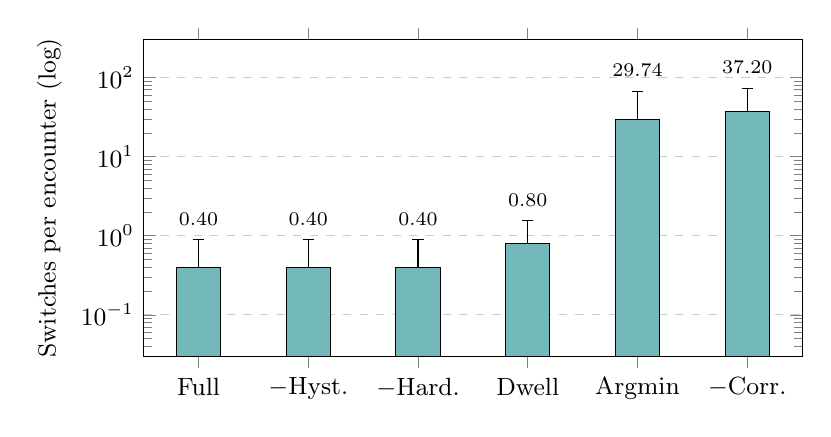
\begin{tikzpicture}
\begin{axis}[
  width=0.82\linewidth, height=5.6cm,
  ybar, bar width=16pt, ymode=log, log origin=infty,
  ymin=0.03, ymax=300,
  xtick={0,...,5}, xticklabels={{Full},{$-$Hyst.},{$-$Hard.},{Dwell},{Argmin},{$-$Corr.}},
  ylabel={Switches per encounter (log)},
  ymajorgrids, grid style={dashed,gray!40},
  error bars/y dir=plus, error bars/y explicit,
  enlarge x limits=0.1, tick label style={font=\small}, label style={font=\small},
]
\addplot[fill=teal!55, draw=black, error bars/.cd, y dir=plus, y explicit] coordinates {
(0,0.4000) +- (0,0.4909)
(1,0.4000) +- (0,0.4909)
(2,0.4000) +- (0,0.4909)
(3,0.8000) +- (0,0.7498)
(4,29.7440) +- (0,36.7008)
(5,37.2000) +- (0,36.1198)
};
\node[font=\scriptsize,anchor=south] at (axis cs:0,1.0245) {0.40};
\node[font=\scriptsize,anchor=south] at (axis cs:1,1.0245) {0.40};
\node[font=\scriptsize,anchor=south] at (axis cs:2,1.0245) {0.40};
\node[font=\scriptsize,anchor=south] at (axis cs:3,1.7823) {0.80};
\node[font=\scriptsize,anchor=south] at (axis cs:4,76.4115) {29.74};
\node[font=\scriptsize,anchor=south] at (axis cs:5,84.3178) {37.20};
\end{axis}
\end{tikzpicture}
\caption{\textbf{Class-switch count per encounter by variant} (mean with $+$SD whisker, log scale; $N=250$ per variant, 5 scenarios $\times$ 50 seeds, 10.0~s horizon), regenerated with pgfplots from \texttt{ablation\_raw.csv}. The immediate-argmin policy and the synthetic correspondence-loss stress comparator ($-$Corr.) yield 29.74 and 37.20 decision changes per encounter, respectively, whereas the proposed method (Full) maintains commitment with 0.40. Removing hysteresis ($-$Hyst.) or progress hardening ($-$Hard.) alone shows no observed regression in this scenario set, supporting the accumulator configuration's suppression of fluctuations in this scenario set; the synthetic comparator does not identify the causal effect of correspondence.}
\label{fig:oscillation}
\end{figure}


\noindent\textbf{Strongly confirmed findings.} (i) \textbf{Oscillation control (core claim).} The immediate-argmin and synthetic correspondence-loss stress comparators produce about 98 decision changes per encounter in the ambiguous-tie scenario, whereas the proposed method maintains commitment at 0 (\cref{fig:oscillation}; \cref{tab:main,tab:scenario}). The two distributions do not overlap in range (proposed method entirely 0 vs. $-$accumulator 98.16$\pm$7.85, non-overlapping observed ranges), so the observed separation is complete within these runs, not a statement about distributional support. Because the core separation in this offline measurement is categorical, a formal test would not change the conclusion, so we omit one here; Mann-Whitney U tests, effect sizes, and confidence intervals are reported for the physical performance metrics of the Planned Evaluation (\cref{app:planned}). (ii) \textbf{Spurious-input suppression.} In the transient-spike scenario, the proposed method has 0 switches (spike ignored), while argmin has 2 (entering and returning). (iii) \textbf{Rapid commitment.} In the clean-advantage scenario, the proposed method has 1 switch, with t-legible 2.37 s. (iv) \textbf{Legibility.} The oscillatory variants are frequently illegible because the posterior fails to stabilize (argmin and synthetic $-$class censoring 72/250 and 71/250, respectively; \code{near\_tie} t-legible 7.9 s vs. 0.05 s for the proposed method; \cref{tab:legibility}).

\subsection{Ablation Studies}\label{subsec:ablation}

\begin{figure}[t]
\centering
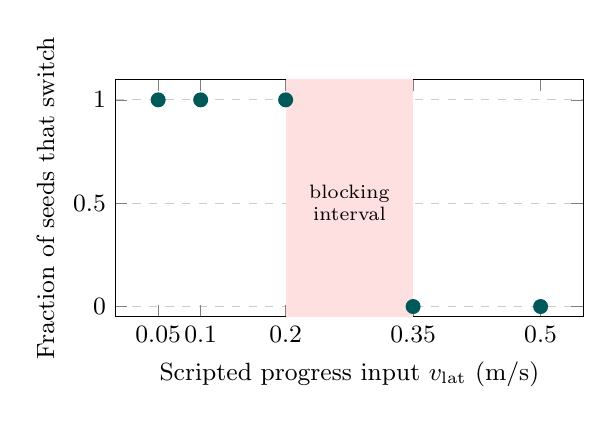
\begin{tikzpicture}
\begin{axis}[
  width=0.62\linewidth, height=4.6cm,
  xmin=0, xmax=0.55, ymin=-0.05, ymax=1.1,
  xlabel={Scripted progress input $v_{\mathrm{lat}}$ (m/s)},
  ylabel={Fraction of seeds that switch},
  xtick={0.05,0.10,0.20,0.35,0.50},
  xticklabel style={/pgf/number format/fixed, /pgf/number format/precision=2},
  ymajorgrids, grid style={dashed,gray!40},
  tick label style={font=\small}, label style={font=\small},
]
\fill[red!12] (axis cs:0.20,-0.05) rectangle (axis cs:0.35,1.1);
\node[font=\scriptsize,align=center] at (axis cs:0.275,0.5) {blocking\\interval};
\addplot[only marks, mark=*, mark size=2.5pt, teal!70!black] coordinates {(0.05,1.00) (0.10,1.00) (0.20,1.00) (0.35,0.00) (0.50,0.00)};
\end{axis}
\end{tikzpicture}
\caption{\textbf{Offline transition blocking under fast progress saturation} (\texttt{clean\_commit}, Full, 50 seeds per point, measured only at the five marked inputs; data from \texttt{R5\_rho\_sweep.md}). Every seed commits the warranted switch for $v_{\text{lat}}\le0.20$~m/s and none does for $v_{\text{lat}}\ge0.35$~m/s, so the transition-blocking interval is $v_{\text{lat}}\in(0.20,0.35)$~m/s. This is a sensitivity of the scripted progress input, not a physical freezing threshold.}
\label{fig:rhosweep}
\end{figure}


\noindent\textbf{Knob ablations: findings that diverged from the prior hypothesis (correction by measurement).} $-$Hysteresis ($\Dfloor = 0$) and $-$progress hardening ($k_\rho = 0$) showed \textbf{no observed regression} relative to the proposed method in these scenarios. Because the leaky accumulator's threshold $E_0$ and leakage already reject zero-mean noise, the primary oscillation-suppression mechanism in this operating regime is not $\Dfloor$ or $k_\rho$ but the \textbf{accumulator} itself. In other words, the earlier revision's preregistered hypothesis that ``$-$hysteresis $\to$ switch-count blowup'' does not hold under the leaky-accumulator design, and this is a \textbf{hypothesis correction} provided by the ablation measurements. In \code{intermittent}, the proposed method switches once at 1.55--2.10 s across the 50 seeds (\code{src/compass\_eval/results/README.md}) and has 0/50 censored trials, with mean t-legible 4.11 s. The earlier report of 50/50 censoring resulted from floating-point posterior saturation, not a late-horizon switch. Computing the same observer in log-odds space removes this numerical absorbing state without changing the decision policy or observer likelihood. In the same scenario, simple dwell never completes the justified switch because intermittent advantage keeps resetting the timer (0 switches), but because it remains in the initial \Class, it is immediately legible to the observer (0/50 censored, t-legible 0.05 s) --- a case where the legibility figure alone masks the switching failure. Simple dwell's total censoring (50/50) occurs not in \code{intermittent} but in \code{mid\_reversal} (after the mid-course switch, the posterior fails to re-stabilize by the end of the horizon), whereas in the same scenario the proposed method maintains commitment (0 switches) and is immediately legible with 0/50 censoring. However, the proposed method's zero switches in \code{mid\_reversal} is the flip side of this same masking effect --- at the default knobs, the accumulator fails to track a late-horizon reversal (in the scenario script, the challenger advantage rises to $+0.25$, i.e., $5\times\Dfloor$, by the end of the horizon; verified at \code{harness.hpp:56}), which is consistent with the conservatism cost noted in \cref{subsec:switch} and the offline transition-blocking sensitivity measured below. \Cref{prop:p2live} makes this quantitative rather than a masking artefact: at the default knobs a discretionary switch at $\rho = 0$ is reachable only for a sustained advantage exceeding $0.23$ (\cref{rem:resptime}), and even at $D_{\text{sus}} = 0.25$ the response-time bound is $N_{\text{resp}} = 76$ cycles ($3.8$ s); the scenario's advantage ramps linearly from $-0.25$ to $+0.25$ over the $10$ s horizon, so it exceeds $0.23$ only in the final $8$ cycles ($0.4$ s), and driving the noiseless ramp through the leaky recursion leaves $\Erev \approx 0.21 < E_0$ at the end of the horizon. The measured $0$ switches is therefore what the analysis predicts for this scenario at these knobs, and the open question it leaves is a knob-design one (a lower $E_0$ improves responsiveness at the cost of the P2 margin; increasing $\lambda$ reduces leak but leaves the stated P2 lower bound unchanged), not a hidden failure of the mechanism. Finally, the t-legible and censoring-rate figures in this section, obtained from the decision-stream proxy observer of \cref{subsec:setup}, measure the stability of the decision stream, not an independent axis of motion legibility, as already noted.

\noindent\textbf{$\rho$-rate sensitivity and offline transition blocking.} The effect of progress hardening depends strongly on the $\rho$ drive rate. Measuring in the scripted \code{clean\_commit} decision-core harness while raising its progress input $v_{\text{lat}}$ from 0.05 to 0.50 m/s, the proposed method always commits (\cref{fig:rhosweep}) (50/50, t-legible $\approx$ 2.4 s) for $v_{\text{lat}} \le 0.20$ m/s, but \textbf{switching is blocked (0/50) for $v_{\text{lat}} \ge 0.35$ m/s}. This is because a rapidly saturating $\rho$ raises $\Eth$ to $E_0(1+k_\rho) = 0.60$, blocking even justified switches --- the clip obstruction in \Cref{prop:p2live} gives a noise-independent blocking mechanism: with the scenario's advantage of $+0.40$ the leak equilibrium is $(0.40-\Dfloor)\,dt/(1-\lambda) = 0.583 < 0.60$, in the noiseless constant-advantage model; independently, the clip bound $e_{\max}=0.50<0.60$ blocks every discretionary switch after saturation regardless of noise, whereas at $\rho = 0$ the same advantage switches within $N_{\text{resp}} = 24$ cycles ($1.2$ s). Whether the switch wins the race against the rising threshold before saturation is precisely what the sweep measures; the \textbf{offline transition-blocking interval is $v_{\text{lat}} \in (0.20, 0.35)$ m/s}. This is a sensitivity of the scripted input and the core's former simplification $v_{\text{lat}}=|v_{\text{cmd}}|$; it does not demonstrate robot immobility, physical freezing, or goal failure. It motivates separating measured cross-track progress from forward speed (\code{compass\_eval/results/R5\_rho\_sweep.md}).

\subsection{Real-Time Performance and Enumeration Complexity}\label{subsec:latency}

\begin{table}[t]
\centering
\caption{\textbf{Historical decision-core timing} of \texttt{DecisionCore::step} (enumeration, cost integration, safety test and decision), 20{,}000 iterations per condition on an AMD Ryzen 5 5500GT, all $2^K$ labels enumerated in an all-safe fixture. Finite-batch measurements, not a worst-case execution-time bound and not an end-to-end ROS~2 pipeline measurement.}
\label{tab:latency}
\small
\begin{tabular}{ccrrrrr}
\toprule
$K$ & Labels $2^K$ & Mean ($\mu$s) & p50 ($\mu$s) & p99 ($\mu$s) & Max ($\mu$s) & Max / 50 ms \\
\midrule
1 & 2 & 1.6 & 1.5 & 2.6 & 153.6 & 0.31\% \\
2 & 4 & 5.4 & 5.2 & 7.9 & 356.1 & 0.71\% \\
3 & 8 & 15.9 & 14.5 & 58.6 & 651.3 & 1.30\% \\
\bottomrule
\end{tabular}
\end{table}


\noindent\textbf{Enumeration complexity (analytical bound).} The current core enumerates $2^K$ labels with $K=\min(N_{\rm people},K_{\rm cap})$ and evaluates each candidate before forming its safe set. At the default $K_{\rm cap}=3$, that is at most eight labels. This is a configured enumeration bound, not evidence that influence ranking, coarse group merging, or a particular pruning distribution has been implemented. The cost of each evaluation also depends on rollout samples, people, and environment queries; the distribution of the resulting $|\mathcal{S}_k|$ in physical scenes remains unmeasured. The ideal pruning/lifecycle design in \cref{subsec:enum} is not a reason to treat the present loop as evaluating only already-safe classes.

\noindent\textbf{$K_{\text{cap}}$ operating rule.} The current implementation retains the first $K_{\rm cap}$ people in input order as explicit class dimensions, with default value 3. It does not compute an influence ranking or merge overflow people into coarse classes. Input selection and ordering therefore matter. Person-cost and safety queries can still examine the supplied people beyond those label dimensions, but that is not a guarantee of a realized passing-side relationship for them.

\noindent\textbf{Historical finite-batch timing.} The archived \code{compass\_eval latency} experiment measured \code{DecisionCore::step} on an AMD Ryzen 5 5500GT with Radeon Graphics for 20,000 iterations per condition, using all $2^K$ enumerated labels and an all-safe environment fixture. The observed p99/max pairs (\cref{tab:latency}) are 2.6/153.6 $\mu$s at $K=1$, 7.9/356.1 $\mu$s at $K=2$, and 58.6/651.3 $\mu$s at $K=3$. The largest observed maximum is about 1.30\% of a 50 ms (20 Hz) period. These are finite-batch measurements, not a proven worst-case execution-time (WCET) bound or an upper bound on deployment latency. The loop evaluates the enumerated candidates before constructing $\mathcal{S}_k$; its work also depends on all supplied people, rollout samples, and environment-query costs, not only $|\mathcal{S}_k|$. Limiting explicit label dimensions does not independently bound all these costs. This historical measurement does not benchmark the new candidate adapter, live costmap access or the end-to-end ROS 2 pipeline (callbacks, TF, controller dispatch, DDS/executor jitter). Those timings and the physical-scene safe-set distribution remain separate evaluation targets.

\section{Discussion and Limitations}\label{sec:disc}

\noindent\textbf{What the Guarantees Cover.} The temporal-consistency claim of \sname\ rests on P2, a deterministic and pathwise lower bound on the interval between discretionary switches that needs only the range bound of the normalized cost and the declared non-vacuity condition \eqref{eq:p2nonvac}; P1(ii) sharpens it to exponential rarity only under an i.i.d.\ hypothesis that stationarity alone does not supply (\cref{rem:dep}). Because P2 is satisfied by a policy that never switches, it is paired with the conditional response-time bound of \cref{prop:p2live}, and the ablations show both sides of that pairing in data: the leaky accumulator suppresses argmin oscillation in \texttt{near\_tie}, while at the same default knobs the late reversal in \texttt{mid\_reversal} is not tracked within the log (an observed outcome that the response bound does not predict, and that only an independent opportunity oracle could score as a miss) and the fast-saturating progress input of \cref{fig:rhosweep} triggers clip-induced lockout (\cref{subsec:ablation}). P3 and P5 are branch-priority and guard contracts, not physical collision-freedom or termination guarantees (\cref{prop:p3,prop:p5}). All of these apply standard dwell-time and CUSUM/queueing arguments (\cref{sec:related,subsec:props}); their value lies in stating, for this rule, the assumptions under which each holds, not in new mathematics.

\noindent\textbf{Cost Analysis.} The historical decision-core timing of \cref{tab:latency} leaves the per-cycle decision computation well inside a 20~Hz period at the default $K_{\rm cap}=3$, but it is a finite-batch measurement of \code{DecisionCore::step} only; the candidate-trajectory adapter, live costmap access, and the end-to-end ROS~2 pipeline are not timed (\cref{subsec:latency}).

\noindent\textbf{Limitations.} (i) The planar (2D) assumption means multi-level or sloped environments are not handled. (ii) Constant-velocity Kalman prediction is strong in the short term but has limits under abrupt intent changes or multi-modal crowds (a learning-based predictor can be substituted as an interchangeable input, \cref{sec:related}). (iii) Front/rear passing is handled only as cost and is not separated into distinct \Class{es}. (iv) The empirical scope of this paper is limited to the decision layer. Behavioral consistency, the decision-stream observer statistic, and per-cycle latency were \textbf{measured} with an offline harness driving the actual decision core (\cref{subsec:main,subsec:ablation,subsec:latency}), but performance metrics requiring physical simulation (success rate, collision, minimum social distance), the external baselines, and the user study have not yet been measured in this evidence set; their protocols have been fixed in advance in the Planned Evaluation (\cref{app:planned}), with per-case values still to be bound before any run. Meanwhile, the ablations showed that the leaky accumulator is the primary oscillation-suppression mechanism (removing $-$hysteresis or $-$hardening alone produced no regression in this regime), and revealed an offline transition-blocking interval for the scripted $\rho$ drive rate ($v_{\text{lat}} \in (0.20, 0.35)$ m/s), not a physical freezing threshold. (v) \textbf{No consistency-weight, opinion-dynamics or closed-loop comparison.} The comparators are internal (immediate argmin, simple dwell, knob ablations and a synthetic correspondence-loss stress comparator). The most direct missing baseline is a previous-class consistency weight~\citep{degroot2024topology,martinezbaselga2026shine} applied to exactly the same candidates and cost streams; opinion-dynamics passing~\citep{cathcart2023opinion} and dwell-plus-relative-improvement selection~\citep{li2026bigcbf} are further baselines. None of these was run and no closed-loop simulation was performed, so the offline results show only that the implemented rule filters scripted, noisy decision-label streams; whether it improves on these mechanisms, or on navigation outcomes, is untested. These comparisons are part of the planned evaluation (\cref{app:planned}). (vi) \textbf{Strength of the guarantees.} At the default knobs the worst-case separation guaranteed by P2 is short (\cref{rem:p2nonvac}), P1 relies on an i.i.d.\ hypothesis that temporally correlated social costs need not satisfy (\cref{rem:iid}), and a policy that never switches satisfies P2; the guarantees are contracts about the decision rule, not evidence of legible or effective navigation. The current contribution is therefore the conditional decision-rule design and formal properties together with \textbf{offline empirical validation of decision-layer consistency}; physical performance, external comparison, and human-data validation are to be filled in subsequently according to the protocol of \cref{app:planned}.

\noindent\textbf{Generalization limits (P4, actuation, sensing).} P4's guarantee of maneuver completion depends on $v_{\text{lat,min}} > 0$ in \cref{asm:scope}(d), which presupposes the following. (i) \textbf{Actuation type.} For nonholonomic drives (differential, Ackermann), cross-track progress is realized only as the product of forward speed and steering, so $v_{\text{lat,min}} > 0$ requires \textbf{positive forward speed and forward clearance}. That is, if the robot stops or the front is blocked, the lateral progress rate becomes 0, breaking P4's premise, and the safety layer (P3, P5) takes over. For holonomic (omnidirectional) drives, direct lateral motion is possible even while stationary, relaxing this premise. (ii) \textbf{Footprint.} The corridor-width and pruning analysis in this paper assumes a circular footprint approximation; a rectangular footprint (an elongated body) has an occupied area that varies with orientation during rotation, which can make corridor-availability determination and the realization of $v_{\text{lat,min}}$ more conservative. (iii) \textbf{Dependence on forward speed.} As noted in (i), $v_{\text{lat,min}} > 0$ depends on forward speed, so in congested environments with frequent low-speed or stopped intervals, the upper bound $K$ on maneuver-completion time increases. (iv) \textbf{Sensor modality.} This design receives person tracking, F-formation, and vulnerable-pedestrian attributes from external modules; 2D-laser-based tracking has weak heading and attribute estimation, whereas depth/RGB-D-based tracking is richer. The quality of $\sigma_{\text{front}}/\sigma_{\text{rear}}$ regime determination and of group/attribute recognition therefore depends on sensor modality, and the guarantees of this paper's decision layer hold on the premise that these inputs are of adequate quality.

\noindent\textbf{Ethical limitations.} The vulnerable-pedestrian handling of \cref{subsec:groups} relies on external attribute classification, which carries risks of bias, privacy, and stigma. This paper specifies only a policy of choosing conservative defaults under uncertainty and does not claim the fairness of the classifier itself as a contribution, and it explicitly notes that a separate ethics and privacy review is needed for real deployment.

\noindent\textbf{Future work.} Carrying out the Planned Evaluation (\cref{app:planned}) --- physical-simulation performance metrics, independently tuned comparison against the external baselines, and validating time-to-legible against human data via the user study --- is the top priority; beyond that, we propose extending front/rear passing into explicit \Class{es} via spatiotemporal $(x,y,t)$ homotopy, and combining the approach with learning-based prediction.

\section{Conclusion}\label{sec:concl}

This paper proposes a decision-layer planner for social navigation that treats the temporal consistency of passing decisions as a first-class objective, combining an ID-indexed, cross-cycle-correspondent representation of \Class\ (a design contract that the current implementation only partly realizes) with a commitment switching rule based on leaky evidence accumulation --- a rectified, leaky variant of Page's one-sided CUSUM statistic~\citep{page1954cusum} with a progress-dependent threshold --- and a lexicographic safety override of the standard priority-arbitration kind. We state five properties (P1--P5): P1 and P2 follow from standard CUSUM/queueing and dwell-time arguments, P3 and P5 are branch-priority and guard contracts, and P4 is a progress-rate and accumulator-containment argument; none is new mathematics. The anti-oscillation guarantee we claim is the deterministic, pathwise inter-switch bound P2 --- at least $N_{\min} = \lceil \Eth(\rho)/((D_{\max}-\Dfloor)\,dt)\rceil$ cycles between discretionary switches for fixed $dt$ (for variable measured intervals, as in the Nav2 adapter, only the accumulated-time form is claimed; \cref{rem:vardt}), zero post-switch evidence, and a range bound on the challenger advantage, informative under the declared condition $E_0 > (D_{\max}-\Dfloor)\,dt$ that the default knobs satisfy --- paired with the conditional response-time bound of \cref{prop:p2live}: its deadline requires the same eligible challenger to remain selected, uninterrupted updates without reset or HOLD, a sustained advantage lower bound, and sufficient clip/leak-equilibrium headroom. P1 states the sharper probabilistic form --- a per-cycle switching probability and per-unit-time switching rate exponentially small in $\theta^* E_0$, obtained by dominating the rule with the Lindley (CUSUM) recursion and applying Kingman's bound, with $\theta^*$ the exact Lundberg root of the increment law (the closed form $\theta^* \approx 2\Dfloor/(\sigma_D^2\,dt)$ is tuning guidance only, and the per-unit-time bound carries a factor of $1/dt$) --- as a refinement conditional on an i.i.d.\ hypothesis on the challenger advantage, since bare stationarity with zero mean and bounded variance admits a counterexample that defeats the exponential form. We also prove P4 on top of the dynamics of progress $\rho$, a lower bound on lateral progress rate, and a \textbf{containment condition on the challenger accumulator $\Erev$} ($\bar\rho$). In particular, the switching dynamics close over the \textbf{single-challenger accumulator} of \cref{subsec:switch}/\cref{subsec:algo}, and the two-sided condition on its reachable upper bound $E_0 < \Eremax < E_0(1+k_\rho)$ --- the lower bound providing algebraic reachability headroom at $\rho=0$ and the upper bound being P4 containment --- replaces any above-threshold headroom requirement $e_{\max} > E_0(1+k_\rho)$, which would contradict P4 containment; the reachability-headroom condition is necessary for any discretionary switch from zero evidence but is not by itself a liveness guarantee, since actual response also requires the persistent-selection, uninterrupted-update and advantage hypotheses of \cref{prop:p2live}, and the clip $e_{\max}$ can separately lock out switching at high progress. On the empirical side, using an offline harness that drives the actual decision core, we measured anti-oscillation behavior (about 98 oscillations per encounter in the ambiguous-tie scenario for the immediate-argmin comparator, vs. 0 for the proposed method and also 0 for the 0.6~s simple dwell, so that scenario separates filtering from no filtering; the accumulator and the dwell differ in the transient-spike, mid-reversal and intermittent scenarios), a decision-stream observer statistic ($t_{\text{sfx}}$ and its right-censoring rate; not a validated legibility measure), and real-time performance ($K=3$ p99 58.6 $\mu$s, max 651.3 $\mu$s; the max is about 1.30\% of the 20 Hz budget) (\cref{subsec:main}, \cref{subsec:latency}), and also obtained, by measurement, an offline transition-blocking sensitivity interval for progress hardening ($v_{\text{lat}} \in (0.20, 0.35)$ m/s); this is not a physical freezing threshold. The comparison that would test whether evidence accumulation improves on existing mechanisms --- previous-class consistency weights~\citep{degroot2024topology,martinezbaselga2026shine}, opinion-dynamics passing~\citep{cathcart2023opinion} and, in concurrent work, dwell-plus-relative-improvement selection~\citep{li2026bigcbf} --- and closed-loop evaluation remain planned (\cref{app:planned}).

\section*{Acknowledgments}

We thank OmniLink for an external rerun that exposed the standard-library dependence of the offline harness. AI tools assisted with translation from the Korean manuscript and with editing; the author verified all technical content and takes full responsibility. An open-source implementation of \sname\ (the decision core, the Nav2 controller plugin, the Gazebo testbed, and the \code{compass\_eval} offline evaluation harness) is available at \url{https://github.com/kjungmo/compass}.

\bibliography{main}
\clearpage
\appendix
\section{Reproducibility}\label{app:repro}

\noindent\textbf{Software and evidence versions.} The integration targets ROS 2 Jazzy; planned physical simulation targets Gazebo Harmonic. ROS build/test evidence is distinct from experiment provenance: R3 is the archived AMD Ryzen 5 5500GT decision-core latency measurement, not a new integrated-controller or ROS-pipeline timing result. Current R1 observer outputs were regenerated on AMD EPYC 9V74. The canonical manuscript source is \code{paper/arxiv/main.tex}, of which this document is a re-typeset edition built from \code{paper/arxiv\_ref}; \code{scripts/build\_paper.sh} uses pdfLaTeX from TeX Live (including science/extra packages), Poppler and ripgrep. Its \code{--check} mode builds in a temporary directory, and \code{--write} deliberately regenerates the PDF and artifact-hash manifest; visual QA is still required. A rerun must record its actual compiler, standard library, TeX/package versions, hardware, flags and commands rather than infer them from the ROS distribution alone.

\noindent\textbf{Build and run commands.} Run from the repository root. The full package build below requires a sourced ROS 2 Jazzy environment and the declared Nav2/simulator dependencies; an evaluator-only build can instead use \code{--base-paths src --packages-up-to compass\_eval}. These commands preserve the archived measurements.

\begin{verbatim}
# Full workspace, including the simulator package (not a simulator run)
colcon build --base-paths src sim --cmake-args -DBUILD_TESTING=ON
source install/setup.bash
colcon test --packages-select compass_core compass_nav2 compass_eval
colcon test-result --verbose

# Separate rerun CSV; summaries are printed to stdout
mkdir -p /tmp/compass_eval_results
./build/compass_eval/compass_eval ablation /tmp/compass_eval_results
./build/compass_eval/compass_eval latency
./build/compass_eval/compass_eval rho_sweep

# Canonical manuscript build, without replacing tracked artifacts
bash scripts/build_paper.sh --check
\end{verbatim}

\noindent\textbf{Selected legacy/shared defaults.} \Cref{tab:params} summarizes the manuscript's default decision knobs and shared controller settings from \path{src/compass_nav2/config/compass_params.yaml}; it is not an exhaustive parameter inventory, a 1:1 list of \code{compass::Knobs}, or a deployment-validation claim. The retained compatibility knob \code{e\_max\_fwd} does not determine discretionary switching and is omitted. Current controller parameters are read at configuration time in \path{src/compass_nav2/src/compass_controller.cpp}; complete example wiring is in \path{sim/config/nav2_compass.yaml}.

The configure-time research defaults are:
\begin{itemize}
\setlength{\itemsep}{0pt}
\setlength{\parsep}{0pt}
\item \code{use\_measured\_progress=false};
\item \code{use\_candidate\_trajectories=false};
\item \code{progress\_max\_gap=0.25} s;
\item \code{progress\_max\_speed=2.0} m/s;
\item in measured mode, $L_{\rm plan}$ is the anchored planned offset described in \cref{subsec:algo} (no configuration knob); legacy mode keeps $L_{\rm plan}=1.0$~m.
\end{itemize}

The research profile in \path{src/compass_core/include/compass_core/response_profile.hpp} sets $k_\rho=0.5$; it does not enable either adapter flag automatically. Their separate contracts are documented in \code{RESPONSIVENESS.md} and \path{docs/CANDIDATE_TRAJECTORIES.md}.

\begin{table}[t]
\centering
\caption{\textbf{Selected legacy/shared default values}; research options and parameter sources are specified in the accompanying text.}
\label{tab:params}
\small
\begin{tabular}{@{}lrp{0.40\linewidth}@{}}
\toprule
Knob & Value & Meaning \\
\midrule
\code{delta\_floor} & 0.05 & Instantaneous switching margin $\Dfloor$ (dimensionless) \\
\code{E0} & 0.30 & Baseline threshold $\Eth(0)$ (normalized-cost seconds) \\
\code{k\_rho} & 1.0 & Progress-hardening coefficient $k_\rho$ \\
\code{p} & 2 & Progress-hardening exponent \\
\code{lambda} & 0.97 & Leak coefficient $\lambda$ per update ($\tau_{\text{leak}} \approx 1.64$ s at $dt=0.05$ s) \\
\code{e\_max\_rev} & 0.50 & Evidence clip $e_{\max}$ (normalized-cost seconds) \\
\code{d\_safe} & 0.5 & Hard safety distance (m) \\
\code{ttc\_min} & 2.0 & Minimum TTC (s) \\
\code{W} & 3.0 & Thrash window length (s) \\
\code{n\_thrash} & 4 & Thrash threshold (count) \\
\code{w\_g}/\code{w\_s}/\code{w\_e}/\code{w\_r} & 1.0/1.0/0.3/0.5 & Cost-term weights \\
\code{sigma\_front}/\code{sigma\_rear}/\code{sigma\_s} & 1.2/0.6/0.5 & Proxemics widths (m) \\
\code{K\_cap} & 3 & Explicit-dimension cap \\
\code{a\_brake} & 0.5 & Acceleration bound (m/s$^2$); speed decrement $a_{\rm brake}dt$ \\
\code{ttc\_stop} & 0.8 & Stop-trigger TTC threshold (s) \\
\code{T\_safe\_dwell} & 0.6 & Safety-dwell protection time (s) \\
\code{eps\_in}/\code{eps\_out} & 0.02/0.06 & Tie entry/exit hysteresis $\varepsilon_{\text{in}}$/$\varepsilon_{\text{out}}$ \\
\code{controller\_frequency} & 20.0 & \code{controller\_server} cycle rate (Hz) \\
\code{max\_linear\_speed} & 0.5 & Linear-speed hard cap (m/s) \\
\code{cruise\_speed} & 0.45 & Default cruise speed (m/s) \\
\code{max\_angular\_speed} & 1.0 & Yaw-rate cap (rad/s) \\
\code{goal\_decel\_dist} & 0.6 & Deceleration-start distance near goal (m) \\
\code{lookahead\_dist} & 1.0 & Local-goal lookahead distance (m) \\
\code{k\_e}/\code{k\_theta}/\code{k\_side} & 3.0/3.0/0.4 & Path-tracking cross-track error, heading, lateral-bias gains \\
\bottomrule
\end{tabular}
\end{table}


\noindent\textbf{Scenario and seed specification.} The offline measurements of \cref{sec:exp} are run over 5 scenarios (\code{near\_tie}, \code{transient\_spike}, \code{mid\_reversal}, \code{clean\_commit}, \code{intermittent}) $\times$ 50 seeds $\times$ 6 variants, with $dt = 0.05$ s (20 Hz) and a horizon of 10 s (200 cycles). Scenario scripts, variant definitions, and the observer implementation are in \code{src/compass\_eval}.

\noindent\textbf{Source and result provenance.} This manuscript accompanies the reviewed integration candidate in \url{https://github.com/kjungmo/compass}; it does not assert that the candidate is already merged into \code{main}. Record the exact checked-out commit and source/configuration/input hashes for every rerun. The original results remain recoverable at \code{9fe495a}; the intermediate log-odds-only observer is identified by PR~12 commit \code{5343d457}; current R1 adds the separately declared, post-hoc 0.30 s follow-up rule. Raw CSVs of all three versions and the per-row comparison are kept in \code{src/compass\_eval/results/observer\_versions/}; the result-version record is \code{src/compass\_eval/results/README.md}. Current behavioral values are in \code{ablation\_raw.csv} and \code{R1\_ablation.md}; \code{R3\_latency.md} and \code{R5\_rho\_sweep.md} retain their distinct archived scope. Conceptual figures are generated from their scripts, not empirical raw trajectories. The labelled-cell \code{scripts/check\_observer\_results.py} and numeric \code{scripts/check\_paper\_numbers.py} verify their declared checks, not every scientific claim. \code{src/compass\_eval/results/PROVENANCE.md} records the SHA-256, producing command and source revision of every committed result file, including the raw CSVs, and \code{scripts/check\_repo\_consistency.py} recomputes those hashes; \code{paper/arxiv/artifact\_manifest.json} records source/PDF/figure hashes for the built manuscript snapshot; any submission tag is a separate future release action.


\noindent\textbf{Reproduction.} From a fresh ROS workspace, build the evaluator and its workspace dependencies with \code{colcon build --base-paths src --packages-up-to compass\_eval}. Run its \code{ablation} mode with output directory \code{/tmp/compass\_rerun} for a separate CSV and stdout summary; \code{latency} and \code{rho\_sweep} print their summaries. Do not overwrite archived results when reproducing. Figure sources are in \code{paper/figures/scripts}; archived latency is machine/toolchain dependent and is not expected to reproduce exactly. The repository README and result-provenance record give the maintained commands and evidence versions.

\section{Notation}\label{app:notation}

\begin{table}[h]
\centering
\caption{\textbf{Principal symbols.} Units follow \cref{subsec:cost}: costs, advantages and margins are dimensionless; evidence quantities carry normalized-cost--second units.}
\label{tab:notation}
\small
\begin{tabular}{@{}lp{0.72\linewidth}@{}}
\toprule
Symbol & Meaning \\
\midrule
$k$, $dt$, $h_k$ & Control cycle index; fixed cycle interval; measured interval at cycle $k$ \eqref{eq:hk} \\
$\mathcal{C}_k$, $\mathcal{S}_k$ & Candidate topological \Class{es}; safe/available subset \eqref{eq:safe} \\
$c^*_k$, $c'_k$ & Committed \Class; selected challenger \\
$J_k(c)$, $w_X$ & Normalized weighted class cost \eqref{eq:cost}; term weights \\
$D_k$, $D_{\max}$ & Challenger advantage $J_k(c^*_{k-1})-J_k(c'_k)$; its range bound \\
$\Dfloor$ & Instantaneous switching margin \\
$e_k$ ($\Erev$) & Single challenger evidence accumulator \eqref{eq:accum} \\
$x_k$, $q_k$, $r_k$ & Pre-test evidence; stored post-reset evidence; evidence after a pre-update reset \\
$\lambda$, $e_{\max}$ & Leak coefficient; evidence clip \\
$E_0$, $\Eth(\rho)$ & Baseline threshold; progress-hardened threshold \eqref{eq:eth} \\
$\rho$, $k_\rho$, $p$ & Maneuver progress; hardening coefficient and exponent \\
$\Eremax$, $\bar\rho$ & Reachable evidence bound \eqref{eq:eremax}; containment threshold \\
$N_{\min}$, $N_0$ & Discretionary inter-switch cycle bounds \eqref{eq:nmin} \\
$N_{\rm resp}$, $D_{\rm sus}$ & Response-time bound \eqref{eq:nresp}; sustained advantage lower bound \\
$X_k$, $\theta^*$ & Driving innovation $(D_k-\Dfloor)dt$; Lundberg root \\
$W$, $N_{\rm thrash}$, $C_W$ & Thrash window; HOLD threshold; window event count \eqref{eq:window} \\
$v_{\text{lat}}$, $v_{\text{lat,min}}$ & Cross-track progress rate; its assumed lower bound (\cref{asm:scope}) \\
$t_{\text{legible}}$, $p^*$ & Time-to-legible \eqref{eq:tlegible}; posterior threshold \\
\bottomrule
\end{tabular}
\end{table}

\section{Extended Results}\label{app:extended}

\Cref{tab:legibility} gives the per-scenario decision-stream endpoint-suffix time $t_{\text{sfx}}$ and censoring counts behind the aggregate $t_{\text{sfx}}$ and censoring columns of \cref{tab:main}.

\begin{table}[t]
\centering
\caption{\textbf{Endpoint-suffix time $t_{\text{sfx}}$ by scenario} from the decision-stream observer with the post-hoc 0.30~s follow-up rule (mean in seconds; parentheses: right-censored trials out of 50). Censored trials enter the mean at the 10.0~s horizon. These values measure the stability of the decision stream, not motion legibility.}
\label{tab:legibility}
\small
\resizebox{\linewidth}{!}{%
\begin{tabular}{lccccc}
\toprule
Variant & near\_tie & transient\_spike & mid\_reversal & clean\_commit & intermittent \\
\midrule
Full (proposed) & 0.05 (0) & 0.05 (0) & 0.05 (0) & 2.37 (0) & 4.11 (0) \\
$-$Hysteresis & 0.05 (0) & 0.05 (0) & 0.05 (0) & 1.96 (0) & 2.89 (0) \\
$-$Progress hardening & 0.05 (0) & 0.05 (0) & 0.05 (0) & 2.36 (0) & 4.06 (0) \\
$-$Accumulator (argmin) & 7.90 (29) & 0.05 (0) & 9.94 (43) & 0.05 (0) & 0.05 (0) \\
Simple dwell (0.6 s) & 0.05 (0) & 0.05 (0) & 10.00 (50) & 1.15 (0) & 0.05 (0) \\
$-$Class correspondence & 7.98 (32) & 0.05 (0) & 9.88 (39) & 0.05 (0) & 0.05 (0) \\
\bottomrule
\end{tabular}%
}
\end{table}


\section{Sensitivity Analysis Design}\label{app:sensitivity}

The sensitivity of the proxemics and convention parameters is designed as follows. Among these, the $\rho$-drive-rate ($v_{\text{lat}}$) axis of progress hardening has already been measured in \cref{subsec:ablation} as an offline transition-blocking interval, $v_{\text{lat}} \in (0.20, 0.35)$ m/s; measurement of physical freezing and of the remaining axes remains for the Planned Evaluation (\cref{app:planned}).

\begin{itemize}
\item \textbf{$\sigma_{\text{front}}/\sigma_{\text{rear}}/\sigma_s$ sweep.} Each parameter is grid-searched over the range $[0.5\times, 2\times]$ of its baseline value, recording the headline and standard metrics to produce sensitivity surfaces. In particular, we confirm whether increasing $\sigma_{\text{rear}}$ reduces the frequency of rear/blind-spot passing.
\item \textbf{Traffic-side (\code{locale.keep\_side}) reversal.} We measure the performance degradation in environments where the right-preference assumption is false (left-hand traffic cultures) or set to \code{none}. A separate performance-sensitivity curve is drawn against the $w_r$ weight.
\item \textbf{Observer-model parameters ($p^*$, $\Delta_{\text{hold}}$).} We check metric stability against changes in the threshold and hold interval of time-to-legible.
\item \textbf{$e_{\max}\cdot\lambda\cdot k_\rho$.} We check switching-rate, windup, and lockup (as defined in \cref{app:planned}) behavior in regions that violate or satisfy the challenger accumulator's two-sided conditions (reachability headroom $\Eremax > E_0$ --- \cref{subsec:leak}; existence of a nonempty lock region $\Eremax < E_0(1+k_\rho)$, $\bar\rho < 1$ --- P4). In particular, we measure how $\lambda$ shifts the containment threshold $\bar\rho$ via the reachable upper bound $\Eremax = \min(e_{\max}, (D_{\max}-\Dfloor)dt/(1-\lambda))$. \textbf{Knob-tuning guidance (simultaneously satisfying containment vs. switchability).} As discussed in the non-vacuity argument of \cref{subsec:props}, if the leak-equilibrium upper bound $(D_{\max}-\Dfloor)dt/(1-\lambda)$ falls below $E_0$, the reachable upper bound never reaches $E_0$, so no discretionary switch is possible and the P1$\cdot$P2 switching dynamics become vacuous. For example, with $D_{\max}=0.5, \Dfloor=0.05, dt=0.05, \lambda=0.7$, the leak-equilibrium upper bound is $(0.5-0.05)\cdot0.05/(1-0.7) \approx 0.075$, which is smaller than $E_0=0.3$ --- so in the region of short $dt$, small $\Dfloor$, and $\lambda<1$, switching capability can unintentionally vanish. Accordingly, this sweep explicitly marks the $\lambda$, $e_{\max}$ combinations whose reachable upper bound falls within the open interval $(E_0, E_0(1+k_\rho))$, so that a designer can identify the $(\lambda, e_{\max})$ region that simultaneously satisfies containment ($\Eremax < E_0(1+k_\rho)$) and switchability ($\Eremax > E_0$).
\item \textbf{Source of normalization constants.} We compare a pre-calibrated constant (recommended, time-invariant map) against a per-cycle min-max statistic (affine-invariant, unit-covariant, but subject to margin drift), measuring how the effective margin drift of $\Dfloor$ upon changes in the candidate set affects the switching rate and anti-oscillation metrics when the candidate set changes (verification of the drift analysis in \cref{subsec:cost}).
\end{itemize}

Reporting is mandatory for nonparametric tests (e.g., Mann-Whitney U), effect sizes, stated seed/trial counts, and per-seed variance and confidence intervals.

\section{Planned Evaluation}\label{app:planned}

This section specifies a protocol, fixed in advance of measurement, for \textbf{all evaluations that this paper has not yet measured} --- the physical simulation and real-robot setup, physical performance metrics, end-to-end pipeline latency, scenarios, the external baselines and their independent tuning protocol, and the legibility user study. This paper reports no measured values for any of these items. The protocol is not a formal preregistration: seed and trial counts and the per-case oracle values of the physical scenarios are still to be bound before any run. Fixing and publishing it before results exist is intended to limit post-hoc tuning and confirmation bias.

\noindent\textbf{Physical simulation and real-robot setup.} Simulation combines Gazebo/Isaac with a reactive pedestrian model (PedSim-family, social-force-based agents) and is repeated across many seeds. Making people reactive is critical to avoiding freezing artifacts. Real-robot validation is performed on an in-house service-robot platform with real corridor-encounter cases, together with a demonstration of the presentation layer's FSD-style AR trajectory overlay. \textbf{However, this AR overlay demo is an output of the presentation layer, separate from the decision layer that is this paper's contribution; it is presented only as a qualitative demo and is not included in the quantitative evaluation below (separation of the decision-layer contribution from the presentation-layer demo).} The number of seeds, number of trials, and environment diversity will be fixed at measurement time but must be stated explicitly when reported. All quantitative comparisons are required to report per-seed variance and confidence intervals (or bootstrap intervals).

\noindent\textbf{Controlling simulator circularity.} If $J_{\text{social}}$'s social-force-based cost and the pedestrian simulator (PedSim/social force) share the same assumptions, the proposed method may overfit to the simulator's reaction model. To control for this, we (i) also replace the pedestrian model with a \textbf{different family} than $J_{\text{social}}$ (e.g., ORCA-based, replay-based) to cross-check the robustness of results, (ii) separately report the sim-to-real gap using real-robot encounter cases, and (iii) conduct actual pedestrian-participation experiments where possible. These results are reported after measurement; only the design is fixed in this section.

\noindent\textbf{Definition of physical performance metrics (standard metrics).} Success rate, integral of minimum social distance/proxemics intrusion, number of near-misses, physical freezing (defined below), path length, time taken, average speed, human-side disturbance (speed change and detour amount of the reactive person), and lateral jerk, which requires trajectory realization. These are to be filled in as the performance columns corresponding to the measured columns in \cref{tab:main}, together with the headline metrics of \cref{subsec:setup}; no figures are reported before measurement, and no physical performance improvement is claimed until success, collision, minimum clearance and physical freezing have been measured. \textbf{Physical freezing} is an interval in which the measured robot speed stays below a stop threshold for at least a minimum duration while the goal is not reached, clearance is adequate and free motion is warranted, and which is not an intentional yield, a commanded STOP, or HOLD; freezing episodes and duration are reported separately from intentional yields and HOLD intervals. Zero decision switches are never counted as freezing, and switch counts are never used as evidence of its absence. The software scorer \code{scripts/physical\_metrics.py} fixes provisional thresholds (0.02~m/s, 2~s, 0.3~m goal distance, 0.5~m clearance) that still require validation.

\noindent\textbf{Warranted-switch evaluation.} To separate consistency from non-responsiveness (the concern that decision-stream metrics reward a frozen commitment), the planned evaluation scores decisions against a \textbf{warranted-switch oracle} that is defined independently of the algorithm's evidence, threshold and cost $J$ (for example, geometric or ground-truth labels supplied by the evaluator, never generated from \sname's own accumulator). Each oracle opportunity fixes, before the runs, its onset, confirmation time, expiry, target class (the available alternative), decision eligibility, and a response deadline. \textbf{Warranted-switch recall} is the fraction of eligible opportunities in which a discretionary switch to the target class occurs by the deadline and is held for the hold time fixed in advance. \textbf{Response delay} is measured from the oracle onset, not from the onset of the algorithm's own sustained advantage, to that switch; a missing response is right-censored at the deadline, and delays are summarized with censoring (e.g., Kaplan--Meier), never by averaging only the successful responses. \textbf{Lockup} is an eligible opportunity whose warranted target and a safe alternative both persist until the deadline without a response; the lockup rate is lockups per eligible opportunity. Opportunities excluded because of clip lockout, challenger retargeting, safety interruption, an unsafe or unavailable alternative, or an invalid log are reported as counts rather than silently dropped. Validation of the conditional response theorem (whether the hypotheses of \cref{prop:p2live} held and whether its $N_{\text{resp}}$ bound was met) is reported separately from this application-level recall. The independent oracle, integrated robot logging, closed-loop runs and physical freezing trials are external gates that this paper has not met; the offline scorer \code{scripts/evaluate\_opportunities.py} implements only the deadline, hold and censoring contract on scripted traces, with oracle labels supplied separately, and no figures are reported before measurement.

\noindent\textbf{End-to-end pipeline latency.} To complement the decision-core latency measurement of \cref{subsec:latency}, we will measure, on the real ROS 2 stack, the end-to-end latency from subscription-callback receipt to velocity-command output (including TF transforms, costmap access, \code{controller\_server} dispatch, and DDS queueing/executor jitter) and report it as a distribution (p50, p99, max).

\noindent\textbf{Scenarios.} 4 encounter types $\times$ corridor width (narrow/wide) --- head-on confrontation, robot overtaking a person, person overtaking the robot (where the correct behavior for the robot is to hold its lane), and crossing. Additional diagnostic scenarios --- symmetric ambiguous configuration (left/right cost tie, targeting P1), sensor noise/gap flicker (targeting anti-oscillation), narrowing corridor (targeting yield/stop via availability pruning), \textbf{a challenger-tie configuration (targeting the tie-break rule)}, \textbf{an F-formation group encounter (confirming the group is not split)}, and \textbf{vulnerable-pedestrian proximity (confirming conservative passing)}.

\noindent\textbf{External baselines.} DWB (Nav2's default local planner, a memoryless oscillation baseline), TEB (multi-homotopy + switching cost), MPPI, a social-force-based planner, and ORCA/RVO for congestion. (The internal ablation baselines have already been measured in \cref{sec:exp}.)

\noindent\textbf{Independent tuning protocol for external baselines.} To avoid the ``weakened baseline'' criticism, each external baseline is tuned by the following procedure. (i) Tuning is performed by a party \textbf{independent} of the authors of the proposed method (or by an automated tuning script fixed in advance). (ii) Each method is optimized under the \textbf{same scenario set and the same evaluation-metric weighting} (e.g., success rate prioritized, social distance as tiebreaker), with the same tuning budget (number/time of parameter searches). (iii) The scenarios used for tuning and the scenarios used for evaluation are \textbf{separated} (tuning-set / test-set split). (iv) The final parameter values used and the search ranges are fully disclosed in the appendix. \textbf{(v) The proposed method itself is also subject to the same tuning protocol (same tuning budget, same tuning/test split, independent party) --- that is, the proposed method is not separately hand-tuned, and every method under comparison undergoes the same procedure symmetrically.} The comparison results produced by this protocol are reported after measurement; this section fixes only the procedure.

\noindent\textbf{Legibility user-study protocol.} To validate the observer-model proxy of \cref{subsec:observer} with human data, a perceptual experiment is designed as follows (results reported after measurement).

\begin{itemize}
\item \textbf{Stimuli.} Videos of the same encounter scenario driven by the proposed method vs. a comparison method (especially a memoryless baseline) are presented, truncated at time points \textbf{before} the passing side becomes apparent.
\item \textbf{Task.} Participants are asked, at each truncation point, ``which side do you think the robot will pass you on,'' and both the \textbf{accuracy of the response and the time to respond (human time-to-legible)} are recorded.
\item \textbf{Hypothesis.} A committing policy allows participants to predict the passing side (i) earlier and (ii) more accurately than a memoryless policy.
\item \textbf{Analysis.} We report the correlation between the Bayesian observer proxy $t_{\text{legible}}$ of \cref{subsec:observer} and human response times, quantifying the validity of the proxy metric. \textbf{Samples for which $t_{\text{legible}}$ is undefined} (cases where the posterior never stably exceeds $p^*$ by the end of the video, so the passing side is never legible, occurring particularly for oscillatory policies) are treated not as missing but as \textbf{right-censored} data. That is, such a sample's $t_{\text{legible}}$ is treated as censored at the video length $T_{\text{clip}}$ and aggregated within a survival-analysis framework (e.g., Kaplan-Meier estimation, log-rank test), rather than being excluded from a simple average or replaced with an arbitrarily large value.
\item \textbf{Ecological-validity limitation.} While the video-truncation stimulus approach is reasonable for control and reproducibility, legibility judgments from \textbf{third-person observation} through a screen may differ from judgments in an actual \textbf{first-person encounter} with the robot --- an ecological-validity limitation. Accordingly, the results of this protocol are reported as primary evidence, while validation with real pedestrians in first-person encounters must be filled in by a separate, currently unmeasured experiment.
\item \textbf{Ethics and sample.} The number of participants $N$, recruitment and consent procedures, repeated-measures design, and nonparametric tests are to be fixed before data collection.
\end{itemize}

All measured values from the user study (accuracy, timing, correlation, p-values) are reported only after measurement; this item fixes only the operational definitions and procedures.

\end{document}
